%---------------------------------------------------------------------------%
%-                                                                         -%
%-                           LaTeX Template                                -%
%-                                                                         -%
%---------------------------------------------------------------------------%
%- Copyright (C) Huangrui Mo <huangrui.mo@gmail.com> 
%- This is free software: you can redistribute it and/or modify it
%- under the terms of the GNU General Public License as published by
%- the Free Software Foundation, either version 3 of the License, or
%- (at your option) any later version.
%---------------------------------------------------------------------------%
%->> Document class declaration
%---------------------------------------------------------------------------%
\documentclass[twoside]{Style/ucasthesis}%
%- Multiple optional arguments:
%- [<oneside|twoside|print>]% oneside eprint, twoside eprint, or paper print
%- [fontset=<adobe|none|...>]% specify font set instead of automatic detection
%- [scheme=plain]% thesis writing of international students
%- [draftversion]% show draft version information
%- [standard options for ctex book class: draft|paper size|font size|...]%
%---------------------------------------------------------------------------%
%->> Document settings
%---------------------------------------------------------------------------%
\usepackage{booktabs}

\usepackage[number,list]{Style/artratex}% document settings
%- usage: \usepackage[option1,option2,...,optionN]{artratex}
%- Multiple optional arguments:
%- [bibtex|biber]% set bibliography processor and package
%- [<numbers|super|authoryear|alpha>]% set citation and reference style
%- <numbers>: textual: Jones [1]; parenthetical: [1]
%- <super>: textual: Jones superscript [1]; parenthetical: superscript [1]
%- <authoryear>: textual: Jones (1995); parenthetical: (Jones, 1995)
%- <alpha>: textual: not available; parenthetical: [Jon95]
%- [geometry]% reconfigure page layout via geometry package
%- [lscape]% provide landscape layout environment
%- [xhf]% disable header and footer via fancyhdr package
%- [color]% provide color support via xcolor package
%- [background]% enable page background
%- [tikz]% provide complex diagrams via tikz package
%- [table]% provide complex tables via ctable package
%- [list]% provide enhanced list environments for algorithm and coding
%- [math]% enable some extra math packages
%- [xlink]% disable link colors
\usepackage{Style/artracom}% user defined commands
%---------------------------------------------------------------------------%
%->> Document inclusion
%---------------------------------------------------------------------------%
%\includeonly{Tex/Chap_1,...,Tex/Chap_N}% selected files compilation
%---------------------------------------------------------------------------%
%->> Document content
%---------------------------------------------------------------------------%
%-
%-> Titlepage information
%-
%---------------------------------------------------------------------------%
%->> Titlepage information
%---------------------------------------------------------------------------%
%-
%-> 中文封面信息
%-
\confidential{}% 密级:只有涉密论文才填写
\schoollogo[scale=0.095]{ucas_logo}% 校徽
\title{Spark框架缓存管理策略研究}% 论文中文题目
\author{汤瑞}% 论文作者
\advisor{谭光明~研究员~中国科学院计算技术研究所}% 指导教师:姓名 专业技术职务 工作单位
%\advisor{指导教师一\\指导教师二\\指导教师三}% 多行指导教师示例
\degree{硕士}% 学位:学士、硕士、博士
\degreetype{工学}% 学位类别:理学、工学、工程、医学等
\major{计算机系统结构}% 二级学科专业名称
\institute{中国科学院计算技术研究所}% 院系名称
%\institute{中国科学院力学研究所\\流固耦合实验室}% 多行院系名称示例
\date{2021~年~6~月}% 毕业日期:夏季为6月、冬季为12月
%-
%-> 英文封面信息
%-
\TITLE{ Research on Memory and Cache Management in Spark}% 论文英文题目
\AUTHOR{Tang Rui}% 论文作者
\ADVISOR{Supervisor: Professor Tan Guangming}% 指导教师
\DEGREE{Master}% 学位:Bachelor, Master, Doctor, Postdoctor。封面据英文学位名称自动切换,需确保拼写准确
\DEGREETYPE{Engineering}% 学位类别:Philosophy, Natural Science, Engineering, Economics, Agriculture 等
\MAJOR{Computer Architecture}% 二级学科专业名称
\INSTITUTE{Institute of Computing Technology, Chinese Academy of Sciences}% 院系名称
\DATE{June, 2021}% 毕业日期:夏季为June、冬季为December
%---------------------------------------------------------------------------%
%
\begin{document}
%-
%-> Frontmatter: title page, abstract, content list, symbol list, preface
%-
\frontmatter% initialize the environment
%---------------------------------------------------------------------------%
%->> Frontmatter
%---------------------------------------------------------------------------%
%-
%-> 生成封面
%-
\maketitle% 生成中文封面
\MAKETITLE% 生成英文封面
%-
%-> 作者声明
%-
\makedeclaration% 生成声明页
%-
%-> 中文摘要
%-
\intobmk\chapter*{摘\quad 要}% 显示在书签但不显示在目录
\setcounter{page}{1}% 开始页码
\pagenumbering{Roman}% 页码符号

计算机的迅速发展与普及使得人民大众也可以享受丰富的计算机应用与产品。为了解决大规模数据处理规模大、速度慢的问题,新型的分布式存储和计算框架应运而生。Spark框架拓展了早期的Hadoop框架,加入了缓存管理机制以及基于弹性分布式数据集RDD(Resilient Distributed Dataset)的丰富并行运算算子。一方面Spark通过基于内存的分布式计算模型支持了图计算、机器学习、大数据等多种应用。此外,Spark解决了传统Hadoop系统计算速度慢,应用场景单一等问题。优化了批处理、交互式处理、迭代式计算等计算模式中存在的重复访问数据的问题。极大的扩展了这类分布式数据处理框架的使用边界。

缓存管理机制和由RDD组成的DAG(Directed Acyclic  Graph)引擎是Spark的核心。但是Spark框架缺乏有效缓存选择机制,框架没有办法识别并缓存计算过程中发生重用的数据。现有Spark缓存框架存在一下三点问题:第一,数据的缓存操作完全依赖于编程人员;第二,Spark框架的缓存管理策略使用了LRU(Least Recent  Use)策略,LRU策略只考虑数据访问的时间信息,没有考虑Spark应用本身的拓扑信息,包括DAG图结构,作业执行时间等信息;第三,因为缓存管理模块依赖于JVM虚拟机,框架和底层JVM内存释放异步执行会造成了潜在的OOM(Out of Memory)问题。

为了解决上述的三个问题。本文在详细研究分析了Spark框架在缓存管理方面的原理和运行机制后,针对Spark的原理设计实现了优化的缓存管理机制,包括:自动缓存管理模块、基于DAG拓扑结构缓存替换策略和容错新加强的冗余缓存清理模块。从而对上述Spark缓存管理机制中存在的三点问题提出了一体化的解决方案。本文的主要工作如下:

\begin{enumerate}
    \item 设计实现自动缓存系统。为了解决手动指定缓存可能导致的错误缓存、操作复杂的问题,该模块通过提前运行小规模数据集得到重复使用的RDD数据,之后再执行大规模数据集时自动缓存重复使用的RDD数据。此外考虑了新版本Spark中添加的动态执行特性。Spark框架在运行过程中修改执行计划时自动管理模块也会实时修改DAG图信息,本文也会相对应的做出调整,保证能够做出正确的缓存决策。通过这种方式实现了自动缓存的功能。经过测试,对于迭代式计算和SQL作业,自动缓存模块平均额外计算开销占作业总执行时间的12\%和3\%。
    \item 设计实现基于DAG拓扑结构的缓存替换策略。为了优化缓存替换策略,从而加速作业执行速度,该策略综合考虑了RDD的大小、计算代价以及DAG图拓扑结构等特征。综合计算得到RDD数据的优先级,发生缓存替换时淘汰优先级最低的RDD数据。经过测试,对于大规模测试样例,作业平均执行时间减少了23s。
    \item 设计实现了容错新增强的冗余缓存清理模块。为了解决缓存占用率高以及出错情况下作业容错性差的问题,该模块通过对DAG图的分析,在计算过程中自动删除部分冗余的缓存对象,提高内存空间利用率。通过保留距离当前正在计算的RDD数据为2的数据,增加了系统的容错性,从而可以兼顾系统的内存利用率和容错性。经过测试,作业执行过程中的缓存占用率平均降低了19.5\%。
\end{enumerate}

\keywords{分布式计算,Spark框架,缓存管理,缓存策略}% 中文关键词
%-
%-> 英文摘要
%-
\intobmk\chapter*{Abstract}% 显示在书签但不显示在目录

The rapid development and popularization of computers have enabled the general public to enjoy a wealth of computer applications and products.In order to solve the problem of large-scale data processing, a new type of distributed storage and computing framework came into being.The Spark framework expands the early Hadoop framework, adding a cache management module and a rich operator based on the elastic distributed data set RDD.Spark supports a variety of applications such as graph computing, machine learning, and big data through a memory-based distributed computing model. Spark solves the problems of poor performance of traditional Hadoop systems and single application scenarios thus greatly expand the use boundary of this type of distributed data processing framework.

The cache management module and the DAG engine composed of RDDs are the core optimization points of Spark. However, the Spark framework lacks an effective cache selection mechanism, and the framework cannot identify and cache data that is reused during the calculation process.Data caching operation is completely dependent on the programmer.The cache management strategy of the Spark framework uses a simple LRU strategy. The LRU strategy only considers time information, which does not meet the complex background of Spark applications.Because the cache management module relies on the JVM virtual machine, the asynchronous execution of the framework and the underlying JVM memory release will cause a potential OOM (Out of Memory) problem.

In order to solve the above three problems. This paper studies the principle and operating mechanism of the Spark framework analyzed in detail, and designs and implements an automatic cache management module based on the principle of Spark, a cache replacement strategy based on the DAG topology, and a newly enhanced redundant cache cleaning module for fault tolerance.Thus, a set of solutions are proposed for the problems existing in the Spark cache management system. The main work of this paper is as follows:

\begin{enumerat}
    \item This article designs and implements an automatic caching system. This article runs a small-scale data set in advance to get the reused RDD data, and then automatically caches the reused RDD data when executing a large-scale data set. This article also considers the dynamic execution features added in the new version of Spark. When the Spark framework modifies the execution plan during the running process, the automatic management module will also modify the DAG graph information in real time. This article ensures that the correct caching decision can be made.
    \item This article designs and implements a cache replacement strategy based on DAG topology. This strategy comprehensively considers the characteristics of RDD size, computational cost, and DAG graph topology structure. The priority of RDD data is obtained by comprehensive calculation, and the RDD data with the lowest priority is eliminated when cache replacement occurs.
    \item This paper designs and implements a new and enhanced redundant cache cleaning module for fault tolerance. Through the analysis of the DAG graph, this article automatically deletes some redundant cache objects during the calculation process to improve the utilization of memory space.This paper increases the fault tolerance of the system by retaining the data whose distance is 2 from the RDD data currently being calculated, so that the memory utilization and fault tolerance of the system can be taken into account.
\end{enumerate}


\KEYWORDS{Distributed computing, Spark framework, cache management, cache strategy}% 英文关键词
%---------------------------------------------------------------------------%
% title page, abstract
{% content list region
\linespread{1.2}% local line space
\intobmk*{\cleardoublepage}{\contentsname}% add link to bookmark
\tableofcontents% content catalog
\intobmk*{\cleardoublepage}{\listfigurename}% add link to bookmark
\listoffigures% figure catalog
\intobmk*{\cleardoublepage}{\listtablename}% add link to bookmark
\listoftables% table catalog
}
% \intobmk\chapter*{符号列表}% 显示在书签但不显示在目录

% \section*{字符}
% \nomenclatureitem[\textbf{Unit}]{\textbf{Symbol}}{\textbf{Description}}
% \nomenclatureitem[$\Unit{m^{2} \cdot s^{-2} \cdot K^{-1}}$]{$R$}{the gas constant}
% \nomenclatureitem[$\Unit{m^{2} \cdot s^{-2} \cdot K^{-1}}$]{$C_v$}{specific heat capacity at constant volume}
% \nomenclatureitem[$\Unit{m^{2} \cdot s^{-2} \cdot K^{-1}}$]{$C_p$}{specific heat capacity at constant pressure}
% \nomenclatureitem[$\Unit{m^{2} \cdot s^{-2}}$]{$E$}{specific total energy}
% \nomenclatureitem[$\Unit{m^{2} \cdot s^{-2}}$]{$e$}{specific internal energy}
% \nomenclatureitem[$\Unit{m^{2} \cdot s^{-2}}$]{$h_T$}{specific total enthalpy}
% \nomenclatureitem[$\Unit{m^{2} \cdot s^{-2}}$]{$h$}{specific enthalpy}
% \nomenclatureitem[$\Unit{kg \cdot m \cdot s^{-3} \cdot K^{-1}}$]{$k$}{thermal conductivity}
% \nomenclatureitem[$\Unit{kg \cdot m^{-1} \cdot s^{-2}}$]{$S_{ij}$}{deviatoric stress tensor}
% \nomenclatureitem[$\Unit{kg \cdot m^{-1} \cdot s^{-2}}$]{$\tau_{ij}$}{viscous stress tensor}
% \nomenclatureitem[$\Unit{1}$]{$\delta_{ij}$}{Kronecker tensor}
% \nomenclatureitem[$\Unit{1}$]{$I_{ij}$}{identity tensor}

% \section*{算子}
% \nomenclatureitem{\textbf{Symbol}}{\textbf{Description}}
% \nomenclatureitem{$\Delta$}{difference}
% \nomenclatureitem{$\nabla$}{gradient operator}
% \nomenclatureitem{$\delta^{\pm}$}{upwind-biased interpolation scheme}

% \section*{缩写}
% \nomenclatureitem{CFD}{Computational Fluid Dynamics}
% \nomenclatureitem{CFL}{Courant-Friedrichs-Lewy}
% \nomenclatureitem{EOS}{Equation of State}
% \nomenclatureitem{JWL}{Jones-Wilkins-Lee}
% \nomenclatureitem{WENO}{Weighted Essentially Non-oscillatory}
% \nomenclatureitem{ZND}{Zel'dovich-von Neumann-Doering}

% symbol list, preface content
%-
%-> Mainmatter
%-
\mainmatter% initialize the environment
%---------------------------------------------------------------------------%
%->> Main content
%---------------------------------------------------------------------------%
\chapter{绪论}\label{chap:intro}

\section{研究背景与意义}
2000至今,计算机领域有着跨越式的发展。计算机系统已经不仅仅应用于科研、银行、企业等领域,而是融入了每一个人的日常生后之中。从计算机软硬件系统的角度来看,计算机系统由传统的IOE架构,也就是IBM公司生产的小型机,Oracle公司研发的数据库软件,EMC公司研发的高端商用存储发展 成为扩展性、性价比更高的分布式架构。传统IOE架构存在着扩展性差,硬件成本高的问题。这些问题就使得IOE架构无法满足2000年以后蓬勃发展的互联网应用的需求。

为了满足互联网应用数据量大,增长迅速、成本要求严格的要求。各个公司研发了一系列基于廉价硬件的分布式软件系统。其中谷歌公司于2003年至2006年发表的三篇论文:GFS,MapReduce以及BitTable对引领了整个分布式系统领域的发展。GFS(Google File System)这篇论文介绍了分布式文件系统的设计与实现,GFS最大的特点是具有良好的可扩展性,支持大文件存储,并且运行在廉价硬件上,通过多副本的方式提供了容错性,从根本原理上来说,GFS将一个大文件切成很多小块,每一小块数据存储在多个磁盘中,GFS系统解决了大规模数据的存储问题。MapReduce介绍了处理大数据的方法,通过将任务分发到多个计算节点同时计算,最后在Reduce阶段汇总结果从而完成大数据处理。BigTable解决的结构化数据的存储问题。这三篇论文解决了分布式大数据处理领域最核心的三个问题,也启发了众多分布式系统的发展。

在数据处理这一个领域,在2004年MapReduce发表之后,各个公司实验室研发了一系列的数据处理系统。比如雅虎公司研发并开源了Hadoop、HDFS、Hbase三个系统,分别对应MapReduce、GFS、BitTable三个系统。后面基于Hadoop也有一系列的该进。比如Pig、Hive系统添加了对脚本语言和SQL查询语言的支持。微软和阿里巴巴等公司也研发了Scope、Fuxi等大数据系统。这些系统虽然可以处理大规模数据,但是因为要将中间数据存储在HDFS,使得计算速度很慢,也无法满足机器学习,图计算等迭代计算作业的要求。为了解决这些问题,加州大学伯克利分校的AMPLab研发了基于内存计算的分布式数据处理系统Spark,它的主要特点是将中间数据存储在内存之中,这样就可以极大的加快数据处理的速度。和传统的Hadoop系统对比,在Spark的优势项目迭代式计算方面,有着上百倍的性能提升。在作业执行的灵活性上,Spark也做出了很大的该进。比如在执行的过程中,Spark框架会根据运行时的作业信息动态调整作业的执行计划。比如在发生了数据倾斜的情况时,Spark会创建多个task计算大的分区的数据,在处理完毕之后会添加一个union操作合并数据。

对比Hadoop和Spark就会发现,缓存管理系统是Spark相对于Hadoop做出的核心改进。在Spark系统之中,可以在作业执行节点缓存数据,缓存数据的决策是由编程人员实现的。编程人员在编写Spark代码的过程中,如果发现数据会多次访问到,就会调用cache接口缓存数据。调用cache接口之后,spark系统会设置数据的缓存标志为memory,在计算的过程中,经过计算得到数据之后,spark系统会检查缓存标志,根据缓存标志将数据存放在不同位置,比如内存,磁盘或者直接丢弃。这种缓存策略需要编程人员手动指定缓存位置,会在一定程度上增加编程人员的开发负担,减慢软件的开发进度。

另一个方面,对于缓存数据的管理方面,spark使用的是LRU缓存替换策略管理缓存数据。LRU这种策略非常简单,在缓存空间不够用的时候会替换最近没有访问过的数据。这种缓存替换策略是不适合Spark这种复杂的应用场景的。因为Spark作业会生成一个复杂的计算图,计算图中每个节点是数据,每个数据都需要根据计算图的拓扑结构一步步计算得来,每个数据的计算代价也是完全不同的。可见每个节点的数据并不相等,有的数据可以很快重新计算得到,有的数据如果丢失重新计算它的开销是非常大的。而LRU缓存替换策略只考虑了数据访问的时间信息,这就有可能将重新计算开销非常大的数据替换出去,造成作业执行速度变慢。

\section{课题研究内容}

本文将从两个大的方面进行研究。第一个方面,研究Spark自动缓存系统。第二个方面,研究优化Spark缓存管理策略。对于自动缓存系统,本文使用了一种改进的基于二次执行的自动缓存系统。对于缓存管理方面,本文使用了一种容错性加强的缓存清理策略和一种针对Spark系统特点设计的缓存替换策略。

\begin{enumerate}
    \item 对于自动缓存系统,当前的Spark系统需要手动指定缓存数据,这会加大编程人员的思考负担,在程序规模很大的情况下,思考数据使用情况,数据大小,考虑缓存数据是一件很麻烦的事情。所以需要Spark框架能够自动检测需要缓存的数据,做出缓存决策,减轻编程人员的负担。同时还需考虑Spark框架的新特性,因为Spark有动态执行的新特性,自动缓存模块也需要在Spark框架动态执行调整执行计划的时候同时针对性地做出调整,做出正确的缓存决策。
    \item 针对缓存管理模块,目前因为Spark系统使用JVM(Java Virtual Machine)运行,框架与JVM的内存管理是完全隔离的,这就有可能导致JVM的OOM(Out of Memory)错误。为了解决这个潜在的问题,就需要自动清理缓存中的数据。为了保证容错性,在清理数据的时候需要保存一定的冗余,这样在发生错误的时候就可以通过冗余数据恢复计算。所以就需要根据Spark框架的实现原理,合理设计并实现缓存数据的清理功能。对于缓存替换策略,也需要根据Spark框架的原理设计合适的缓存策略。本文根据Spark计算图的拓扑结构以及计算过程中得到的数据综合计算数据权重,根据数据权重从低到高替换数据。提升整个作业的执行速度。
\end{enumerate}

\section{相关工作}
针对Spark系统的优化主要集中在框架优化,参数配置优化,Shuffle优化,任务调度优化,缓存优化这五个方面。下文会对缓存优化进行详细介绍,对其他四个方面也会进行简单的介绍。

对于框架优化,一般是对Spark框架本身进行一系列的优化,对于Spark中的算子就有很多优化方式。比如文献提供了一种新的join方式ApproxJoin,就可以显著提升join操作的效率。英伟达改造了算子的底层实现方式,使用GPU加速算子的执行过程。

对于参数配置优化,是通过调整参数为Spark框架提供合适的运行环境,合理的参数配置会使得Spark框架能够充分利用机器资源。这方面主要通过HBO(History Based Optimization)基于历史统计信息的优化。也有文献将机器学习和参数优化结合起来,提出了一种基于决策树的参数优化方法。

对于Shuffle优化,因为上有节点的数据需要通过Shuffle才能被下游计算节点使用,Shuffle节点会阻塞计算图下游节点的运行。所以Shuffle性能的高低对于整个作业的性能和吞吐量有着巨大的影响。所以有很多针对Shuffle的优化方法。正对Shuffle过程中数据倾斜问题,有文献提出一种针对数据倾斜数据块的优化算法,通过调整shuffle输出的临时文件来改善Shuffle运行时间。还有通过分布式内存优化Shuffle的Alluxio系统等。

对于任务调度优化,M.Zaharia等人提出了一种可以同时解决数据局部性和调度公平性的延迟调度算法。杨志伟等人提出了一种针对异构Spark计算集群的自适应任务调度策略(Heterogeneous Spark Adaptive Task Scheduling, HSATS),HSATS的主要思想是实时检测集群中的状态,并根据状态信息调整作业的分配权重信息,使用权重信息进行任务调度。启发式的算法也被大量应用于异构计算集群作业调度优化领域,例如文献中设计了针对异构计算集群的任务感知调度系统RUPAM,RUPAM使用了一种启发式的算法,根据异构集群的多种特征进行作业调度优化。



\subsection{分布式系统内存管理}

在分布式场景中,大量作业共享计算集群。合理高效的利用计算集群的计算资源不仅对于单个作业的运行性能有着重大影响,同时也成为提高计算集群能效比的关键。所以分布式系统中的资源管理和分配是分布式云场景下需要研究的重要问题。在资源调度管理中,分布式集群的内存管理是分布式系统资源管理和优化的核心问题,尤其对于Spark分布式系统来说,因为Spark是基于内存的分布式计算系统,所以内存管理是提升Spark性能的关键。

Hadoop通过一种静态固定的资源槽(slot)方式管理处理器以及内存资源。Slot中包含一定数量的CPU和内存资源。Hadoop集群资源控制器将整个系统资源分成固定数量的slot,每个slot可以运行一个Map作业或者一个Reduce作业。Hadoop通过slot的方式简化了对资源的管理,运行过程中只需要将slot分配个任务。有很多针对Hadoop这种基于slot的资源管理方式的研究。Jord`a Polo根据Hadoop中运行的作业特点,动态调整slot的数量和资源量,从而可以提高集群的资源利用率。Jord`a Polo还提出了一种保证性能的前提下提高资源利用率的资源调度算法。具体来说会检测当前集群中作业的性能,在满足性能的前提下分配尽量少的资源,从而可以提升集群的资源利用率。

Haoyuan Li实现了Tachyon(改名为Alluxio),Alluxio是一个分布式内存文件系统,位于计算框架与文件系统之间,主要作为文件系统的缓存优化读取速度。比如计算框架的不同作业之间需要交换数据时,一般是通过将数据写入分布式文件的临时文件中,并将文件地址发送给另一个作业,这就会造成很大的文件存取延迟。通过使用Alluxio作为文件系统的缓存,任务将数据写入分布式内存文件系统缓存Alluxio之中,这样就可以避免缓慢的文件系统读取延迟,加速作业的执行速度。不同的任务需要读取同一个文件的时候,也可以将数据缓存在Alluxio内存之中,从而可以避免重复加载文件。Alluxio的这些特性使得它可以极大地提高HDFS的读写速度。也可以让作业端到端执行速度加速4倍。

Bikash Sharma提出了一种细粒度的资源分配策略MROchestrator。MROchestrator改变了Hadoop传统的基于slot的的资源分配方式,因为这种方式每个作业只能使用一个slot内部的处理器以及内存资源。Hadoop集群要根据集群的情况创建多种不同的slot。这种静态的资源分配方式无法很好的满足任务多种多样的资源需求。所以MROrchestrator会检测每个作业的负载情况,并实时做出调整。从而能够更高效率地利用系统资源。相对于静态的基于slot的资源分配方式,MROrchetrator动态资源分配机制可以使作业的平均执行时间减少38\%。集群资源使用效率平均提升25\%。

Danial Warneke等人的研究表明,MapReduce这一类作业具有内存弹性的特点。内存弹性是指内存空间越多,任务的执行速度也会相应变快。内存总量减少并不会导致作业运行出错,只是会让作业执行速度变慢。所以他们提出了一种动态资源申请方法。作业开始执行是会想系统申请作业可以执行的最小资源,称之为保证型共享内存(guaranteed share memory),保证型共享内存在作业运行过程中是保持不变的。除此之外还提出了给予型共享内存(granted share memory)。作业在运行过程中如果需要更多的内存,就可以向集群资源管理器申请给予型共享内存。集群资源管理器根据集群的运行状态决定是否分配资源。当新的作业提交到系统,需要保证型共享内存才能执行任务,集群资源管理器就会回收集群的给予型共享内存。这种动态调度方式可以在保证集群作业公平性的前提下提升集群中内存的使用效率。

Feng Lin等认为,Spark将RDD缓存的工作全都交给编程人员会有潜在的问题。第一,编程人员如果缓存了不必要的数据会造成内存浪费。第二,编程人员如果遗漏了重要数据,没有缓存,会影响到作业的执行速度。第三,程序规模变大时,会给编程人员带来很大的额外负担。所以他们设计了一种自动缓存系统。但是这种策略适用于静态计算图,在新版本的Spark中具有自适应动态执行的特性(Adaptive Execution),这种基于静态计算图的自动缓存方法需要进一步改进。

\subsection{分布式系统缓存替换策略研究}

缓存替换技术主要分为三类,第一类是传统缓存替换技术,第二类是多级缓存替换技术,第三类是代价缓存替换技术。传统缓存替换技术一般只关注缓存的访问时间和使用频率。比如常见的传统缓存替换技术有LRU(Least Recently Used)最近最少使用算法、LFU(Least Frequently Used)最不经常使用算法等。Spark就使用LRU作为其缓存替换策略,这类传统缓存替换策略比较简单,考虑的因素比较单一,在复杂场景下做出的缓存替换策略可能会不太合理。

多级缓存替换技术是在传统缓存技术的基础上发展来的,一般有多个缓存队列。比如K级最近最少使用算法(LRU-K)、有一个FIFO队列和一个LRU队列组成的双队列算法(Two Queues,2Q)、多级队列缓存替换算法(Multi-Queue,MQ)。

代价缓存策略会根据作业的特点和集群的状态综合计算作业的权重,从而可以兼顾作业的运行速度和集群的资源利用率。Y.Z.Geng等人提出了LCS策略,这种策略通过分析作业的依赖关系,根据作业丢失产生的恢复成本决定数据的权重。这种方式可以避免将恢复代价很大的数据替换出缓存,从而可以避免作业运行速度下降。还有人将集群资源利用率,作业执行时间等统一建模为能量函数,将问题转化为数值优化问题,通过优化算法计算是的能量函数最大的数据权重值。

\section{本文的主要工作}

本文主要研究分布式内存计算框架Spark的缓存优化技术,主要针对Spark框架的新特性,研究自动缓存技术。以及缓存管理技术,从而可以提高作业的执行速度。本文将从以下四个方面进行研究:

\begin{enumerate}
    \item 研究研究分析分布式内存计算系统Spark的设计实验机制、资源管理方式和作业调度运行模式。测试并分析Spark内存管理机制的特点和问题。Hadoop和Spark都是基于Map-Reduce编程模式的分布式计算系统。Spark性能优于Hadoop的一个很重要的原因就是Spark的内存管理机制。研究分析Spark的内存管理机制有助于进一步优化Spark系统和Spark应用。计划使用中科院大数据测试BigDataBench数据集测试Spark框架中Shuffle Memory和Storage Memory内存分区的使用特点。
    \item 设计实现针对Spark3.0的自动缓存系统。之前的工作自动缓存工作是通过提前运行小规模数据集得到重复使用的RDD数据,之后再执行大规模数据集时自动缓存重复使用的RDD数据。然而2020年6月发布的Spark3.0添加了动态执行特性。框架会在执行过程中根据数据特点选择合适的执行策略。这就要求需要在运行过程中实时监测应该缓存的RDD数据。
    \item 设计实现一种Spark系统中的缓存替换策略。目前Spark系统中使用的是LRU缓存替换策略。LRU策略仅仅能够利用内存中数据访问的时间特性。Spark系统的内存中存储的RDD还具有分布式存储、大小、计算代价等其他特征。所以需要综合考虑RDD数据的特征以及整个作业的拓扑特征,综合考虑,淘汰其中权值最小的RDD数据。
    \item 缓存清理算法。Spark内存管理依赖与JVM(JAVA虚拟机)内存管理。因为Spark executor是一个JVM进程。使用了固定大小的JVM堆内存。Spark框架和JVM堆内存管理是完全隔离的,Spark框架自身会记录内存使用量。在内存不足时会删除内存中缓存的RDD数据,删除操作仅仅是删除内存对象的引用。实际内存回收依赖于JVM的内存回收机制。JVM定期检测内存对象的引用计数,如果引用计数减少为0说明内存对象可以回收,JVM就会进行实际的内存回收。所以Spark如果发生了缓存替换,JVM内存并未回收的情况就会产生OOM(Out of Memory)错误。所以就需要Spark框架自动提前删除不需要的缓存对象,提高内存空间利用率。在清理的同时也要更具作业的拓扑信息保存一定的冗余信息,以便于作业执行出错时能够使用冗余信息迅速恢复计算。
\end{enumerate}

\section{论文结构}

论文的组织结构如下:

第一章:绪论。主要阐述研究背景和研究意义,并分析了国内外相关研究的现状,介绍了本文的主要工作和文章结构。

第二章:分布式大数据内存计算系统Spark系统实现机制概述。本章会分析阐述Spark系统架构以及任务调度执行流程。重点介绍缓存实现原理和缓存管理机制。并且通过实验分析了缓存管理对任务执行速度造成的影响。

第三章:Spark自动缓存模块设计与实现。本章会阐述自动缓存模块的设计以及实现方法。之前的工作,不适用于目前新版本的动态执行框架,本文提出了一种实时自动缓存框架,最后通过实验对比分析了自动缓存框架的性能。

第四章:一种基于DAG作业运行时信息及拓扑结构的缓存替换策略的设计与实现。本章会提出一种结合了作业DAG拓扑结构以及作业执行信息的缓存计算方法。这种方法综合考虑了多种信息,避免了目前框架使用的LRU算法存在的可能将重要数据替换删除的问题。最后通过实验验证了这种缓存替换策略相对于LRU策略的有效性。

第五章:一种容错性加强的自动缓存清理方法。对于分布式系统,必须要重点保证容错信。对于分布式内存计算系统Spark,它的容错原理是在出错情况下根据DAG拓扑重复计算上游数据。所以如果在出错场景下有可能会造成重复计算,导致任务执行延迟。为了避免这种问题,本文采用了以时间换空间的原理,在缓存中保存一定的冗余信息,在出错场景可以迅速通过冗余信息恢复计算。

第六章:总结与展望。本章总结论文的主要内容,并展望后续工作。

\chapter{分布式计算框架Spark实现机制概述}\label{chap:basic}

本章对Spark实现机制进行了详细的分析,尤其针对作业调度执行过程和缓存管理机制进行了深入的分析。

\section{Spark系统实现概述概述}
Spark是一种基于内存的分布式计算框架。Spark框架分为四层:用户层、作业管理执行层、资源任务调度层、物理执行层。在用户层,用户需要使用框架api编写应用代码,准备输入数据,配置应用参数。用户将这些信息提交给作业管理执行层后,框架会将用户应用转化为具体的作业执行计划,分为逻辑处理计划(数据单元和数据处理依赖关系)和物理执行计划(具体执行计划和阶段)。生成了具体的执行计划之后,框架的资源任务调度层会向集群资源管理器申请资源,资源申请成功后,框架把具体任务和资源绑定,并发送作业执行计划给物理执行层。物理执行层收到作业执行计划之后,会根据作业的配置信息下载应用代码,运行任务并将执行结果反馈给框架。下面会对Spark框架的四层进行进一步的介绍。

\begin{figure}[htbp]
    \centering
    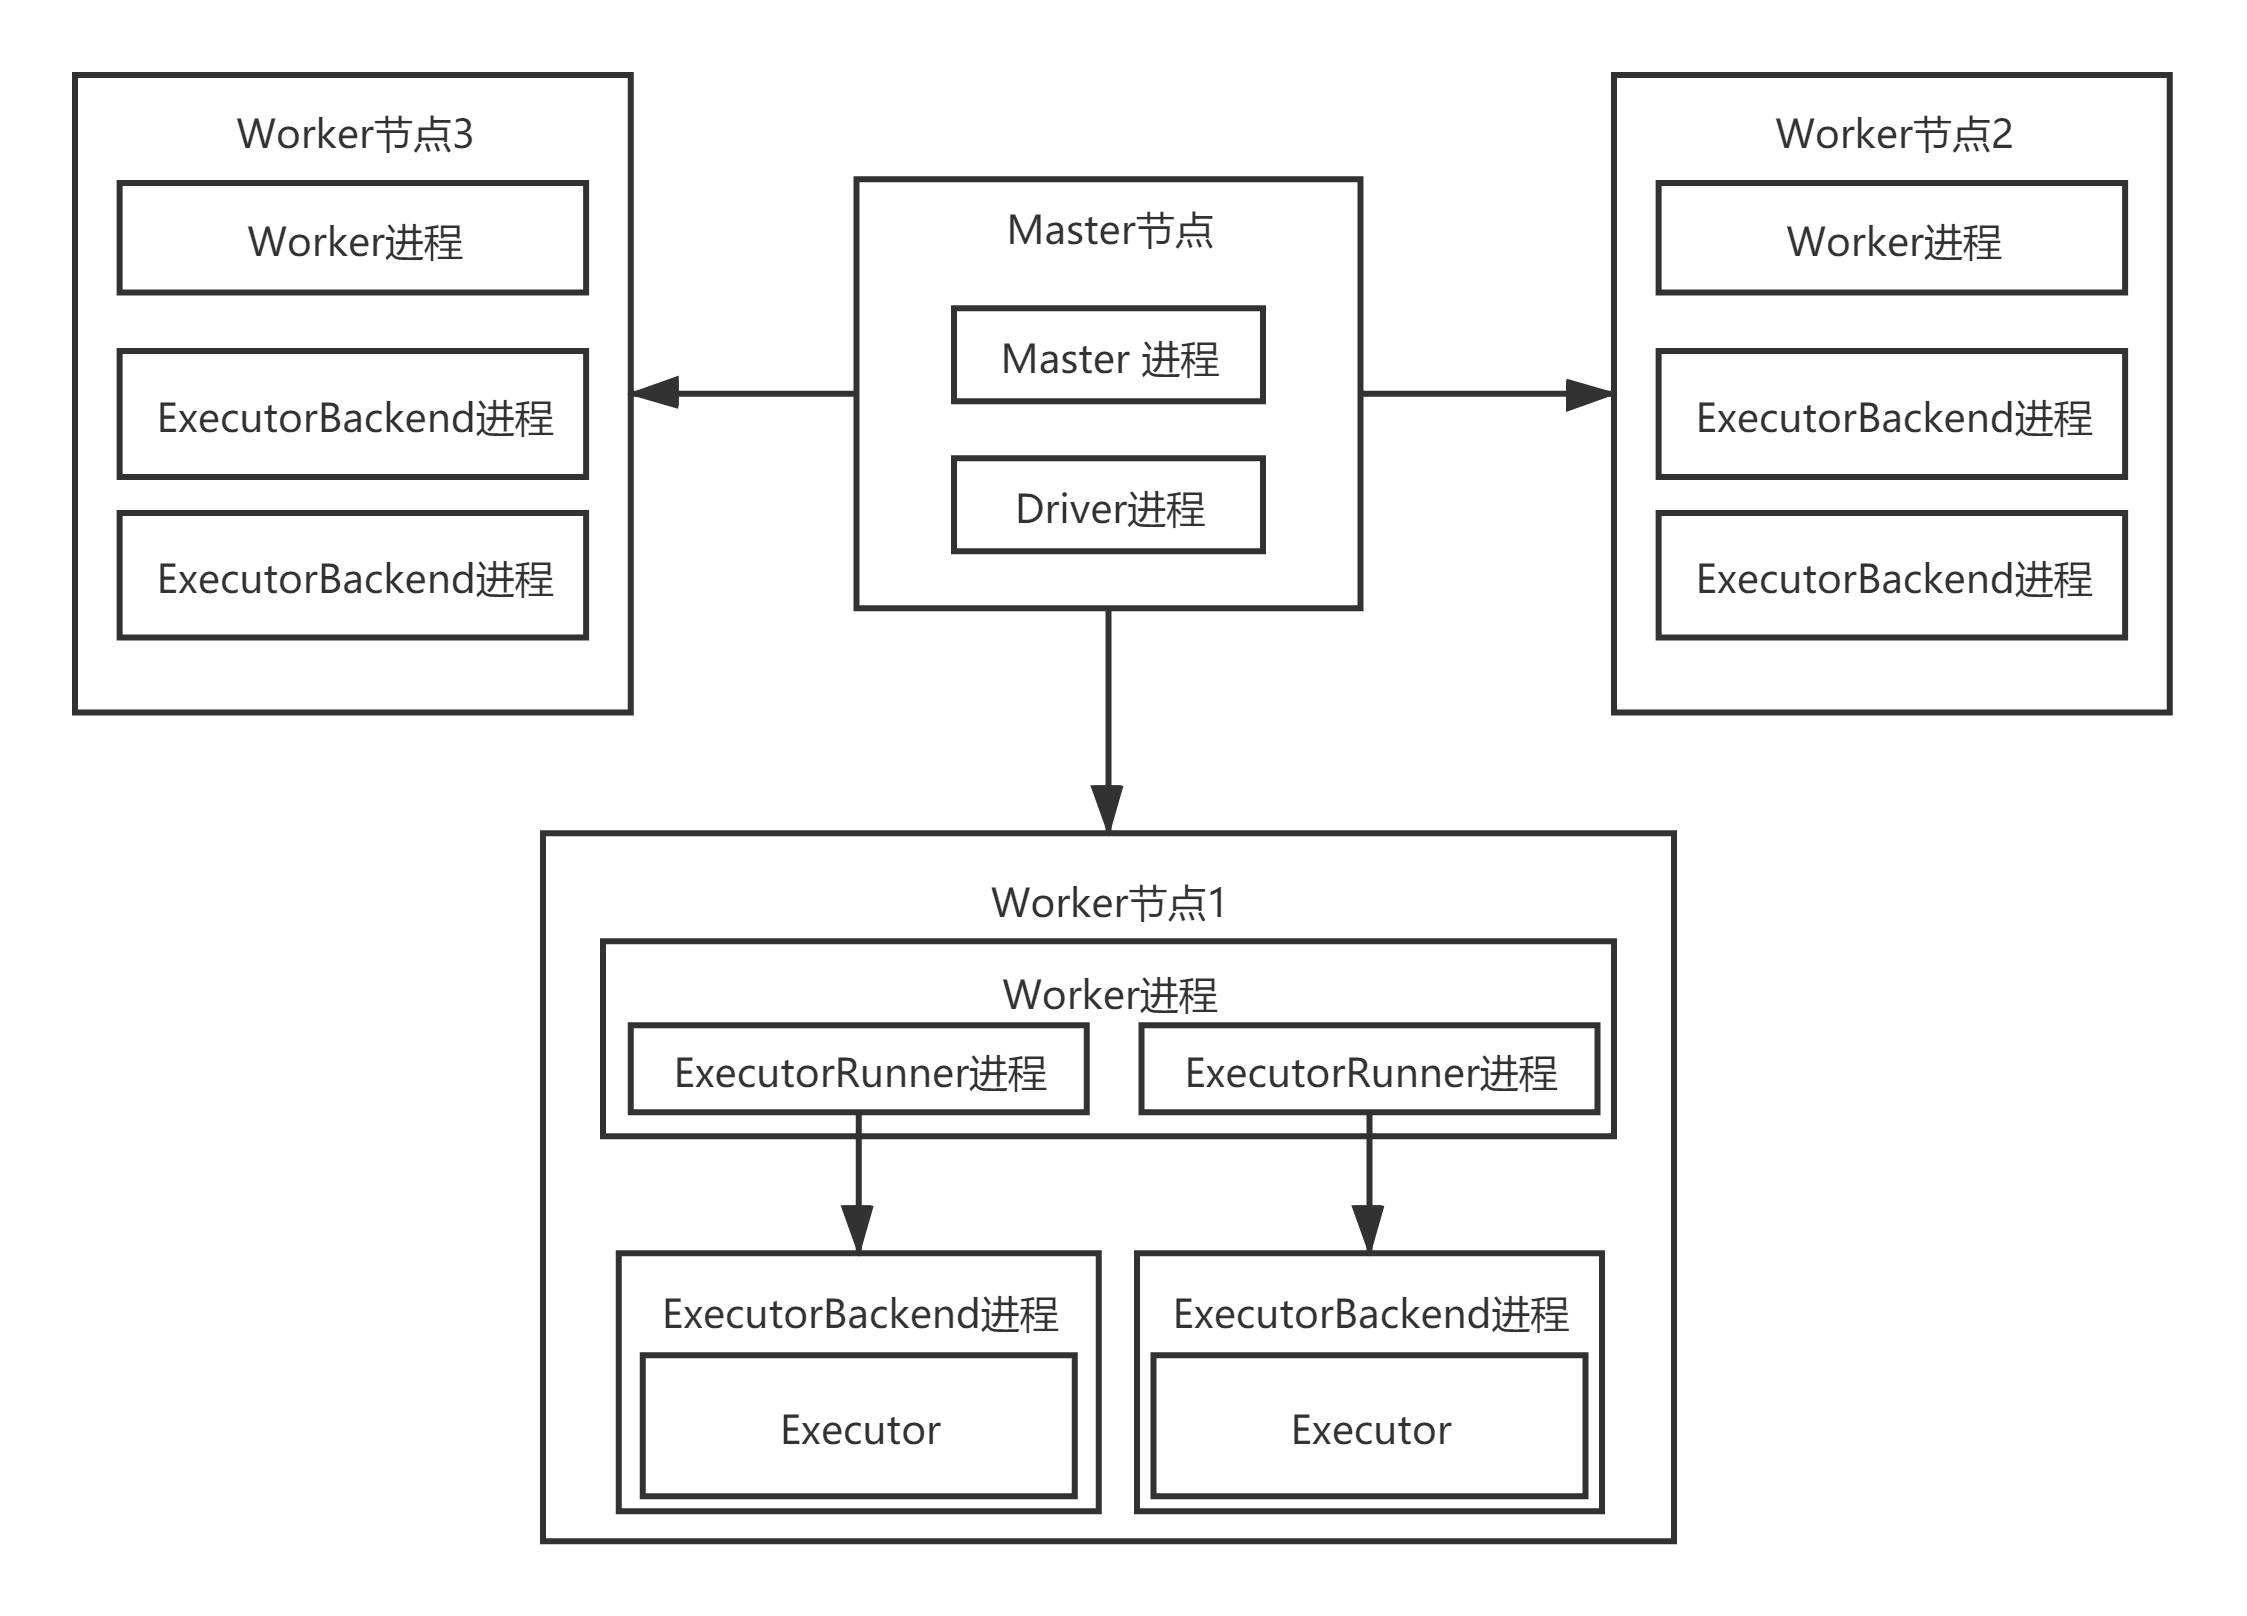
\includegraphics[width=0.99\textwidth]{Img/Spark部署架构图.png}
    \caption{Spark 分布式架构}
    \label{fig:spark-framework}
\end{figure}

\begin{enumerate}
    \item 用户层:用户层提供了丰富的应用接口。包括面向结构化数据的查询接口Spark SQL,面向图计算的GraphX、面向机器学习的Spark MLlib,面向实时流计算的Spark Stream。用户使用提供的接口可以实现丰富的应用程序。
    \item 作业管理执行层:框架收到用户提交的应用程序后,就将其解析成Spark可以识别的逻辑执行计划。比如对于Spark SQL作业,会通过SQL语言的解释器将SQL语句解释为Spark可识别的作业执行计划,一般是以DAG(Directed Acycilc Graph)有向无环图结构组成的作业执行计划。Spark框架会遍历DAG,如果遇到需要Shuffle的边就会对当前边进行切割。遍历完毕之后整个DAG被切割成多个子图,每个子图都会更具拓扑顺序从前到后逐渐调度执行。
    \item 资源任务调度层:Spark框架一般是主从(Master-Slave)架构。主节点负责接受用户的应用,解析作业,管理执行作业,并在出错场景下做容错管理。从节点主要负责接受主节点的任务执行计划,具体执行作业并将结果汇总给主节点。
    \item 物理执行层:物理执行层会执行真正的任务。物理执行层下载或者接受得到用户代码,申请内存开始执行,将执行结果存入特定文件或者通过网络发送给下游节点。任务执行过程中需要内存,输出临时数据也需要在内存中缓存。执行结束之后框架会将执行结果发送给框架。
\end{enumerate}

\section{Spark系统整体架构}
Spark框架系统架构采用了Master-Worker结构。Master节点负责管调度理应用,Worker负责具体执行任务。Master节点会管理监控所有的Worker节点,并且调度执行应用作业,将任务调度给Worker节点,监控收集Worker节点上任务的执行状况。Worker节点会定时和Master节点进行心跳交互。收到Master节点发送的任务后后在本地执行任务,并监控任务状态,将任务执行状况上报给Master节点。具体有一下几个概念需要解释。

Spark Application,Spark应用指的是一个可运行的Spark程序。程序中包含main函数,一般流程是从数据源读取输入数据,进行一系列的处理,计算的到结果后保存到磁盘中。应用程序包含了一些配置参数,例如需要使用的CPU个数,Executor内存大小等。用户可以直接使用Spark提供的接口实现程序,也可以使用Spark SQL编写程序,Spark SQL框架会将SQL查询语言转化成一个Spark应用。

Spark Driver,Spark驱动程序是指运行Spark应用main函数的进程,它会创建Spark Context。一般是指Master节点运行的Spark应用进程,Driver进程独立于Master进程。Driver进程会通过DAGScheduler、TaskScheduler、SchedulerBackEnd等模块调度调度应用中的具体任务。

Executor,Spark执行器是Spark集群的一个资源单位。Spark Driver会向Yarn、K8s等资源调度器申请资源,资源分配成功之后会启动一个Executor进程。之后Spark Driver通过DAGScheduler和TaskScheduler调度执行作业,并通过SchedulerBackend将具体任务发送给Executor。Executor收到任务请求后会在本地JVM虚拟机创建进程执行任务。

\begin{figure}[htbp]
    \centering
    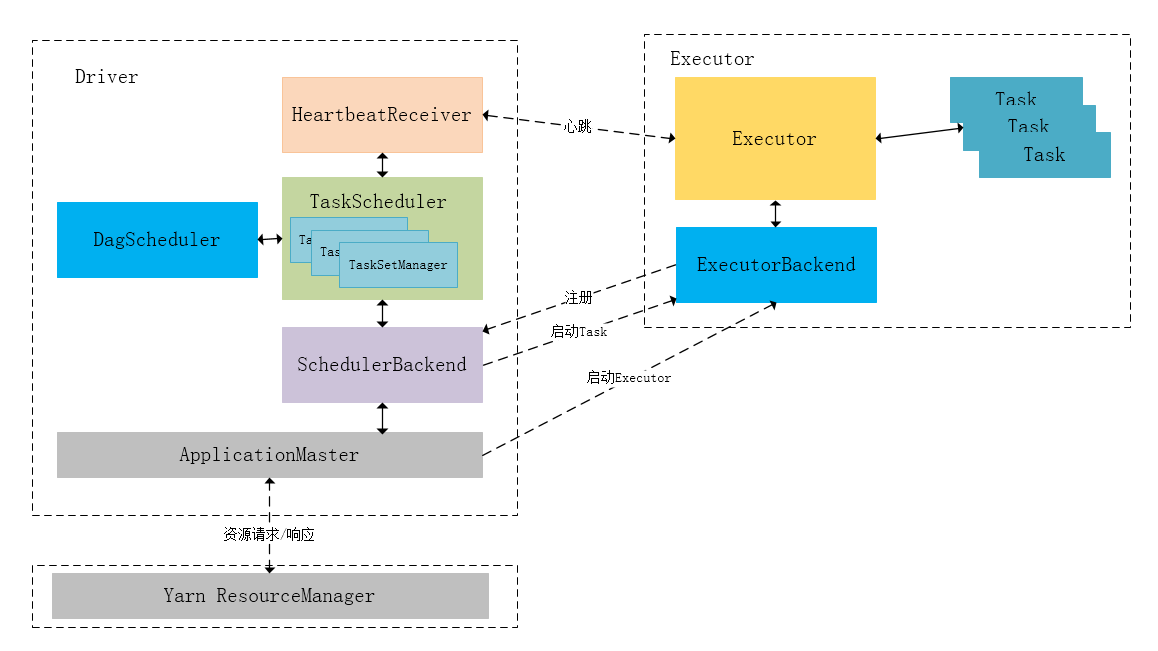
\includegraphics[width=1\textwidth]{Img/spark-scheduler-detail.png}
    \caption{调度执行模块结构图}
    \label{fig:scheduler-models}
\end{figure}

Task,Spark计算任务。Driver程序启动后会将Spark应用切分成多个计算任务,然后调度给Executor执行。Task是最小的计算任务,Executor会给每个Task分配一个JVM进程,执行具体的计算任务,如Map算子、Filter算子、Reduce算子等。Executor一般会占用多个CPU,Task一般使用一个CPU,所以Executor中可以执行多个Task,所有Task共享Executor的内存。

这几个概念中Driver需要进一步解释。Driver包含SparkContext对象,SparkContext会将应用程序转化成一个DAG图,之后遍历DAG图,如果遇到一个action操作,也就是需要具体计算结果的操作,SparkContext就会给DAGScheduler提交一个Job。DAGScheduler收到Job请求之后会从后向前遍历作业,如果遇到边是窄依赖,就会将当前节点加入当前Stage,如果遇到的边是宽依赖,也就是需要Shuffle的边,DAGScheduler就会创建一个新的Stage,并将该节点加入新的Stage之中。遍历结束之后会得到许多个Stage,DAGScheduler会将Stage打包成TaskSet后发送给TaskScheduler执行。TaskScheduler后根据调度策略选择合适的Executor调度执行计算任务。执行结束之后Executor会讲结果汇总发送给Driver。

\begin{figure}[htbp]
    \centering
    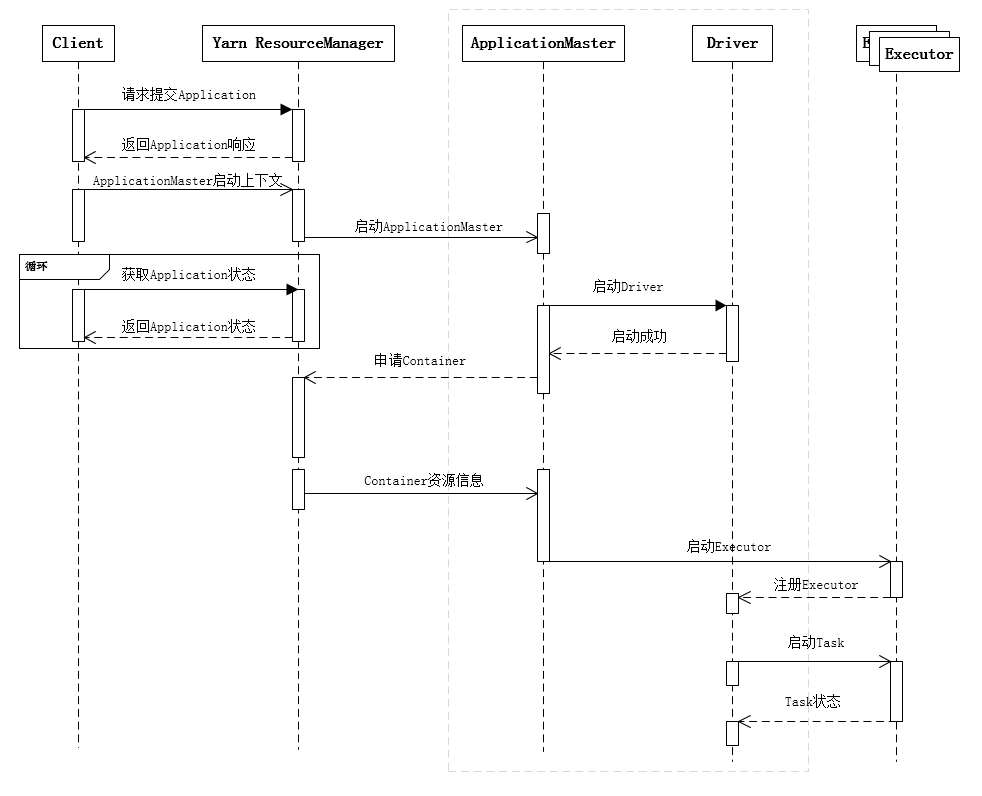
\includegraphics[width=0.99\textwidth]{Img/spark-submit-time.png}
    \caption{Spark应用提交运行流程}
    \label{fig:spark-submit-job}
\end{figure}


\section{作业执行调度模块}

\subsection{作业调度总体架构}
调度模块主要有这几部分:ResourceManager,DAGScheduler,TaskScheduler,SchedulerBackend。其中ResourceManger用于向资源调度器,如Yarn,Mesos,Kubernetes申请资源。资源申请成功之后会启动一个Executor进程。Executor进程启动之后会向Driver进程反向注册,注册成功之后也会持续发送心跳包,同时等待Driver下发任务。收到任务后Executor会执行并上报任务执行状态。这就是资源调度的基本过程。

在任务调度方面,用户的应用程序会根据RDD之间的转化关系转化成一个DAG图,之后框架会将DAG分成多个job,每个job会分成多个stage,stage中的任务会组成taskSet发送给Executor执行,这里详细解释一下这几个概念。

\begin{enumerate}
    \item Application, 用户编写的Spark应用程序,应用提交给Spark框架后框架会将应用转换成框架可以识别的DAG图,并对DAG图进行遍历,遇到action操作时框架就会给DAGScheduler提交一个Job。
    \item Job,action操作会触发job,Driver会将RDD发送给DAGScheduler调度执行。
    \item Stage,每个job根据RDD的宽依赖会分割成多个stage,每个stage中都包括一个TaskSet。
    \item TaskSet,一组没有Shuffle宽依赖的Task集合。DagScheduler会将TaskSet发送给TaskScheduler调度。
    \item Task,RDD中的一个分区对应一个Task,Task是最小的调度执行单位。
\end{enumerate}

\begin{figure}[htbp]
    \centering
    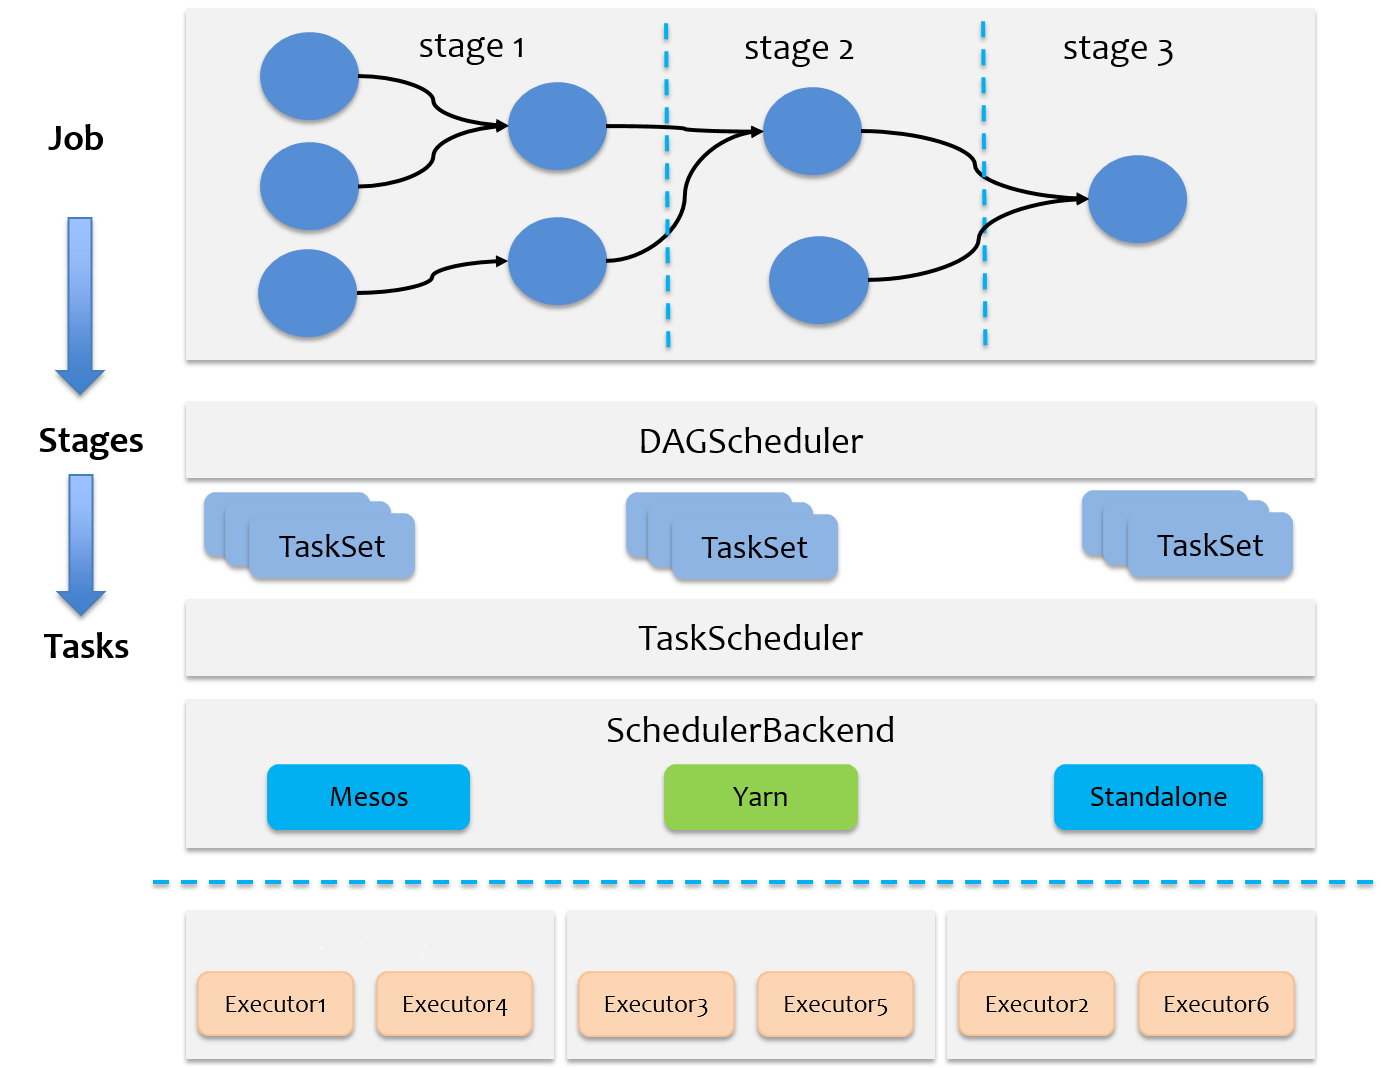
\includegraphics[width=0.99\textwidth]{Img/spark-scheduler-overview.png}
    \caption{Spark应用调度流程}
    \label{fig:application-schedule-process}
\end{figure}

\subsection{调度详细过程}
任务调度可以分为stage级别调度和task级别调度。stage级别调度会先对DAG图进行分割。划分过程是从job的最后一个RDD开始向上回溯遍历,遇到宽依赖,也就是需要Shuffle的依赖就将RDD加入新的Stage之中。如果是窄依赖就将RDD加入当前Stage之中。这样就可以根据依赖关系将一个job切分成许多个Stage。

切分成多个Stage后会根据拓扑排序的关系从前到后执行。当一个Stage的父Stage全都执行完成之后当前Stage就会被调度执行。DAGScheduler会将Stage中Task信息,包括分区信息和操作方法等序列化打包成TaskSet交给TaskScheduler,每个分区Partition都对应一个Task。提交TaskSet之后DAGScheduler会监控Stage执行状况。

\begin{figure}[htbp]
    \centering
    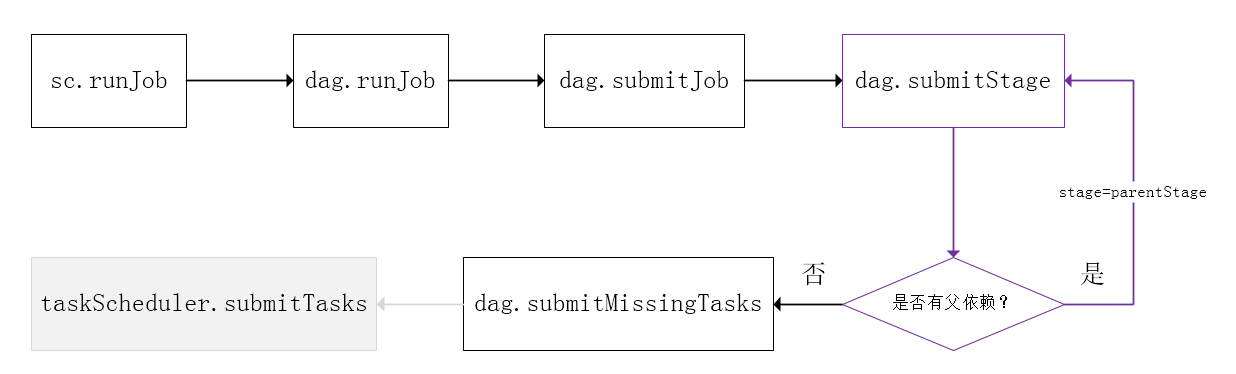
\includegraphics[width=0.99\textwidth]{dag-scheduler-process}
    \caption{DAG调度处理流程}
    \label{fig:dag-scheduler-process}
\end{figure}

Task级别调度是由TaskScheduler完成的。DAGScheduler会将Stage打包成TaskSet发送给TaskScheduler。TaskScheduler会为每一个TaskSet创建一个TaskSetManager来管理TaskSet。TaskScheduler会将新的TaskSetManager加入到队列等待调度执行。TaskScheduler启动之后会启动SchedulerBackend,SchedulerBackend是负责和外界沟通的。ResourceManager申请到资源后会启动Executor。SchedulerBackend负责和Executor通信。包括接受Executor的注册信息,记录Executor的状态。SchedulerBackend管理Executor也就相当于管理这物理资源,SchedulerBackend启动之后会定时询问TaskScheduler有没有任务调度需求。具体来说SchedulerBackend会给SchedulerBackend上报Executor剩余的资源,TaskScheduler会根据资源总量同时根据配置的调度策略调度一定数量的Task执行。

\begin{figure}[htbp]
    \centering
    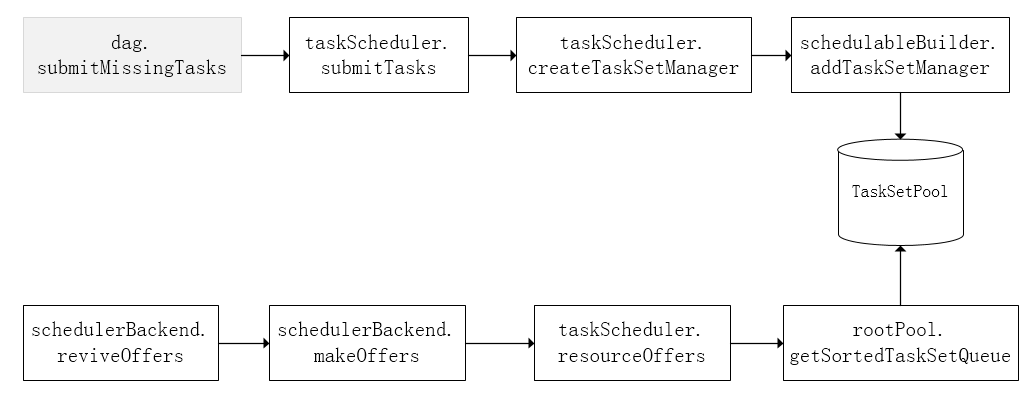
\includegraphics[width=0.99\textwidth]{task-scheduler-process}
    \caption{Task调度处理流程}
    \label{fig:task-scheduler-process}
\end{figure}

TaskSet被封装成TaskSetManager,TaskScheduler通过树形结构管理TaskSetManager。树的根节点类型为Schedule,叶子节点为TaskSetManager,中间非叶节点为Pool。TaskScheduler有两种调度策略,FIFO策略和FAIR策略。使用FIFO策略时TaskSetManager是以先来先出的方式进入队列。结构大概如\ref{fig:scheduler-fifo-tree}所示。

\begin{figure}[htbp]
    \centering
    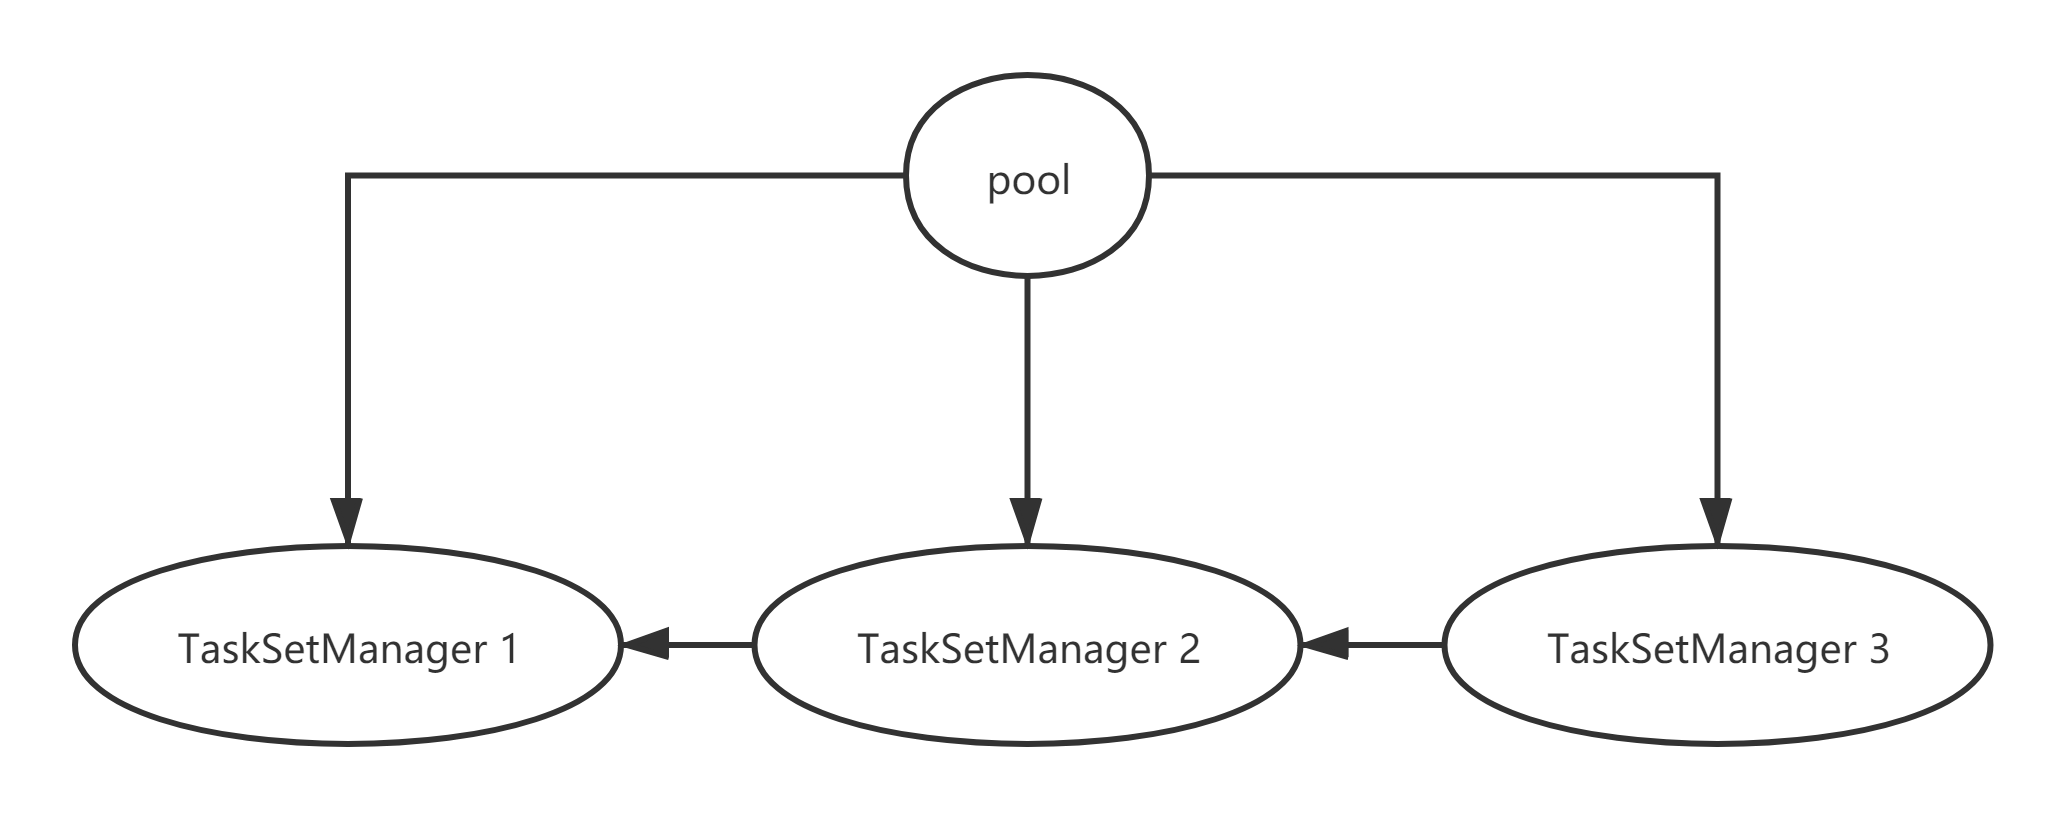
\includegraphics[width=0.99\textwidth]{Img/FIFIO底层策略.png}
    \caption{FIFO调度策略底层树结构}
    \label{fig:scheduler-fifo-tree}
\end{figure}

FAIR调度策略用于保证多个作业的公平调度。比如有两个job,每个job的pool是不同的。FAIR调度会从根开始递归排序,首先对count-pool和take-pool排序。然后再对两个pool内部的TaskSetManager排序。排序的原则会考虑三个属性:runningTasks、minShare、Weight。通过三个属性进行比较的过程比较繁琐,最后能够保证的结果是不让资源被某些task长期占用,从而保证各个作业都能有调度执行的机会。

\begin{figure}[htbp]
    \centering
    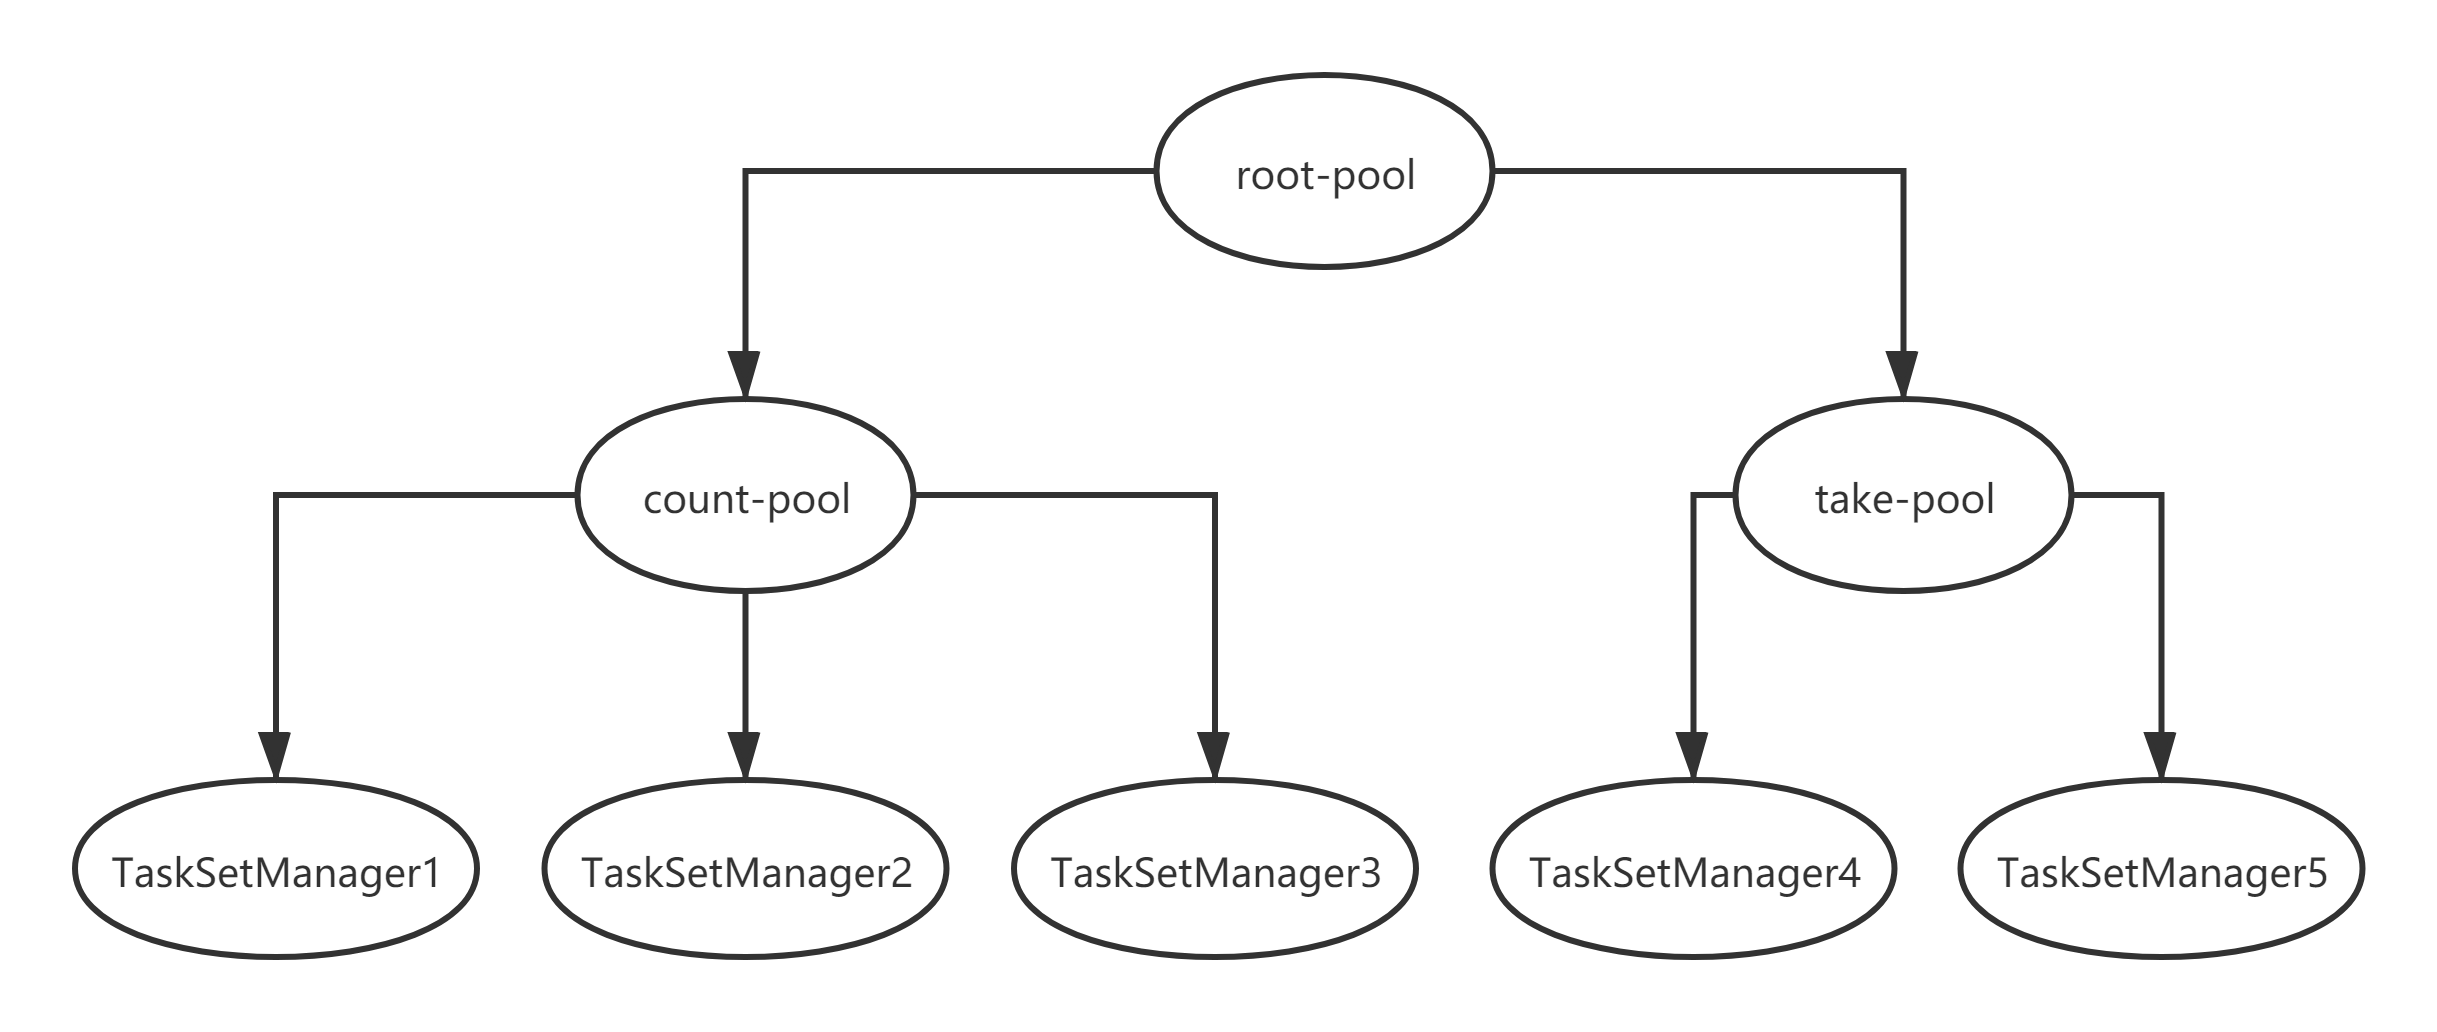
\includegraphics[width=0.99\textwidth]{Img/FAIR底层逻辑.png}
    \caption{FAIR调度策略底层树结构}
    \label{fig:scheduler-fair-tree}
\end{figure}


\subsection{重要算子介绍}

Join算子是Spark最重要的底层算子之一,所以非常有必要单独详细解析join操作的实现原理。Join操作主要有两种使用场景,第一种用于Spark SQL之中,另一种是通过DateFrame编写Spark应用程序。通过语法分析、一系列查询优化之后会得到逻辑执行计划,最后映射为物理执行计划,转化为DAG执行。

Join操作具有三大要素:Join方式、Join条件和过滤条件。Spark支持图\ref{fig:join-overview}所示的6中Join操作,每种Join操作还有不同的实现方式。


\begin{figure}[htbp]
    \centering
    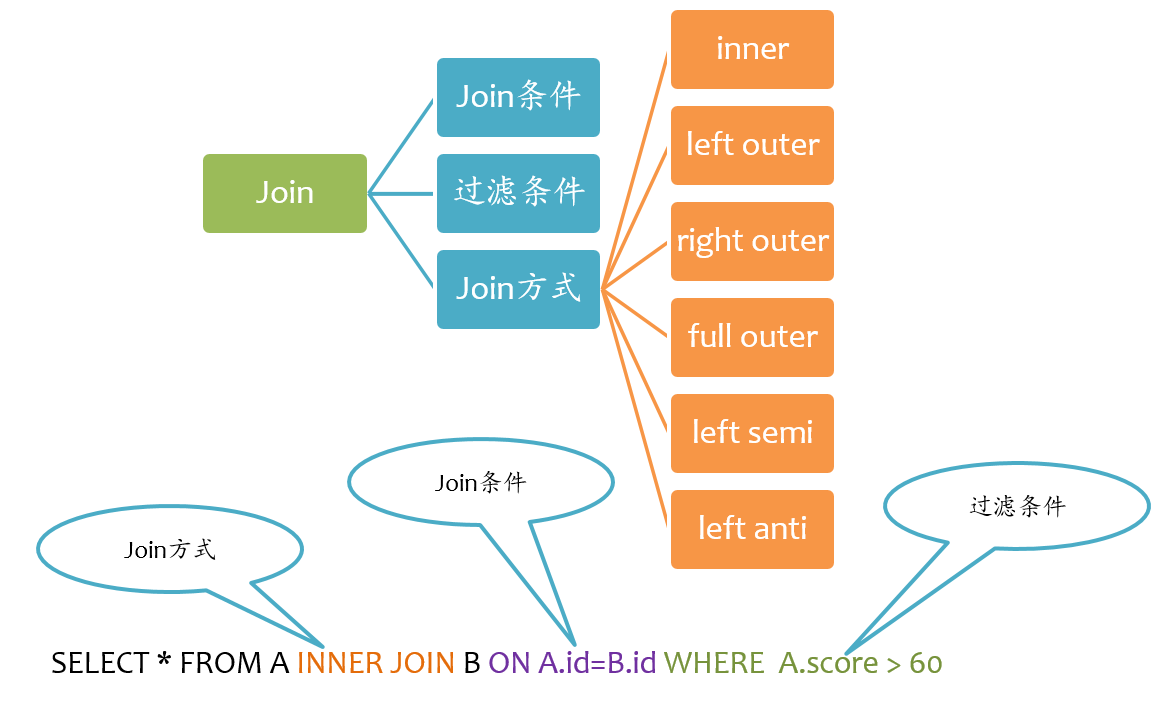
\includegraphics[width=1\textwidth]{Img/spark-sql-join-overview.png}
    \caption{Join操作三要素}
    \label{fig:join-overview}
\end{figure}

Join的基本实现方式如图\ref{fig:join-basic}所示。Spark会将参与Join操作的两张表抽象为流式遍历表(streamIter)和查找表(buildIter)。通常streamIter为大表,buildIter为小表。在计算过程中Spark会遍历streamIter中的每一条记录,每次从streamIter中读取一行记录rowA,根据Join条件计算keyA,然后根据keyA去buildIter中查找满足Join条件(keyA==keyB)的记录rowBs,并将rowBs中每条记录分别与rowA进行指定的join操作得到临时结果,最后根据过滤条件得到最终的join的结果。

根据对join过程的分析可以发现,对于streamIter的每条记录,都要在buildIter中查找匹配的记录,所以buildIter一定需要时查找性能比较好的数据结构。Spark提供了三种Join实现:Sort Merge Join、Broadcast Join以及Hash Join。

\begin{figure}[htbp]
    \centering
    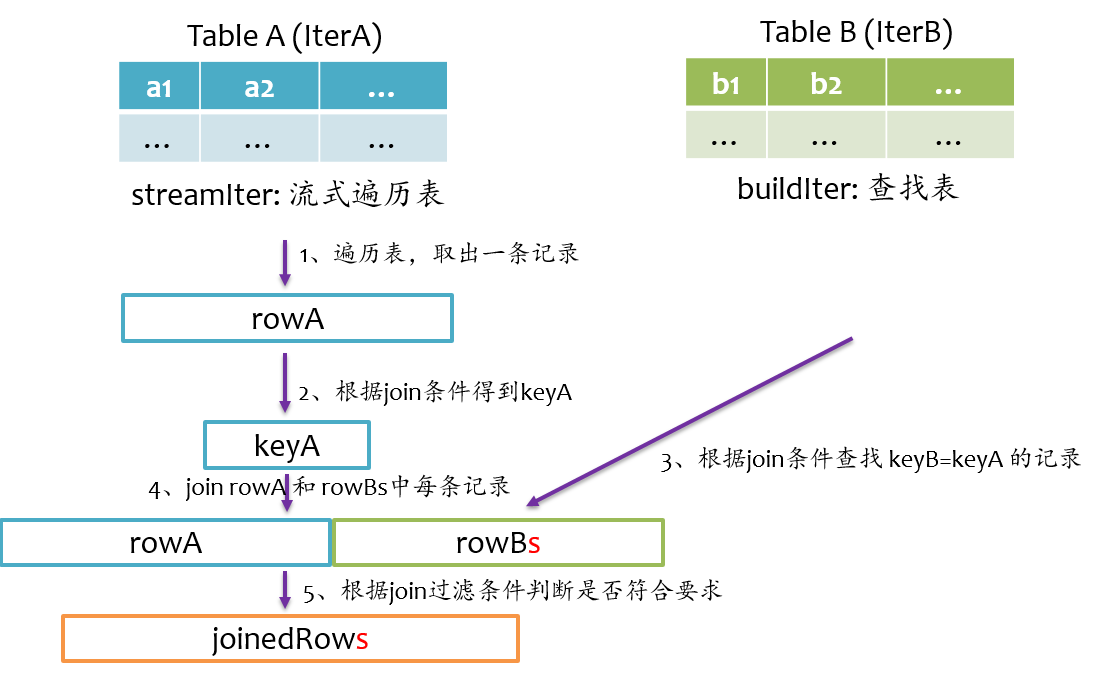
\includegraphics[width=1\textwidth]{Img/spark-sql-join-basic.png}
    \caption{Join操作基本原理}
    \label{fig:join-basic}
\end{figure}

Sort Merge Join实现原理如图\ref{fig:sort-join}所示,join操作要将两条记录合并在一起。首先需要将具有共同key的记录存放在同一个分区之中,所以需要做一次shuffle将具有相同key的记录存放到相同分区之中,map阶段根据join条件确定每个记录的key,使用该key做shuffle write,将可能join到一起的记录分到同一个分区之中,这样在shuffle read阶段就可以将两个表中具有相同key的记录在同一个分区中处理。因为buildIter需要是查找性能比较好的数据结构,一般会自然的想到哈希表,但是对于一张比较大的表来说,因为内存空间相对有限,所以不可能将所有记录存放在hash表中。也可以对buildIter进行排序,查找时通过二分查找,这样查找代价为$O(log_n)$, 查询代价也是比较小的。根据上一节对shuffle原理的分析可以发现Spark目前使用的SortShuffle本来就会对partition中的数据排序。所以buildIter经过shuffle之后是排序完成的,直接使用二分查找就可以迅速找到buildIter中的记录。在shuffle read阶段,分别对streamIter和buildIter进行merge sort,在遍历streamIter中的记录时,对于每一条记录都采用二分查找从buildIter中查找对应的记录,由于两个表都是排序的,每次处理完streamIter的一条记录后,对于streamIter的下一条记录,只需要从buildIter中上一次查找结束的位置开始顺序查找,所以不需要每次都在buildIter中进行二分查找,假设streamIter记录数为M,buildIter记录数为N。那么sort merge join的时间复杂度实际为$O(M+N)$,性能是非常好的。

\begin{figure}[htbp]
    \centering
    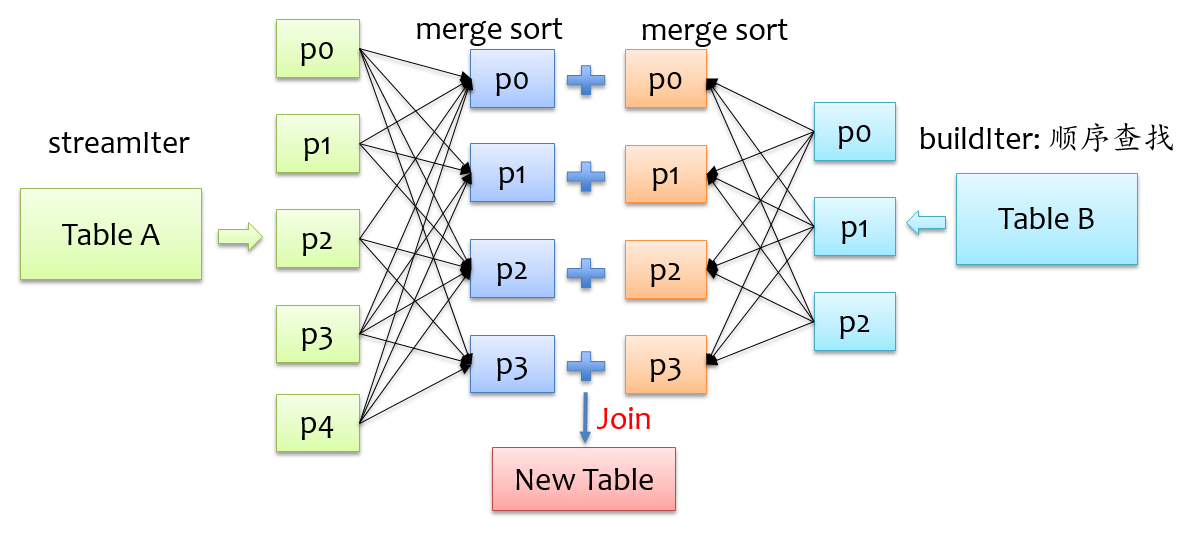
\includegraphics[width=1\textwidth]{Img/spark-sql-sort-join.png}
    \caption{sort Join实现原理}
    \label{fig:sort-join}
\end{figure}

Broadcast Join使用了全新的思路,具体过程如图\ref{fig:broadcast-join}所示。为了能将具有相同key的记录分配到同一个分区之中,一般需要使用shuffle实现,但是在buildIter是非常小的表的场景下,那么就没有必要通过shuffle操作实现,因为shuffle的计算代价是非常大的。在buildIter非常小的情况下,可以直接将buildIter广播到每个计算节点,然后将buildIter放在hash表中。通常这种join被称为map join。当buildIter的估计大小不超过参数$spark.sql.autoBroadcastJoinThreshold$设定的值(默认为10MB),就会自动采用broadcast join。


\begin{figure}[htbp]
    \centering
    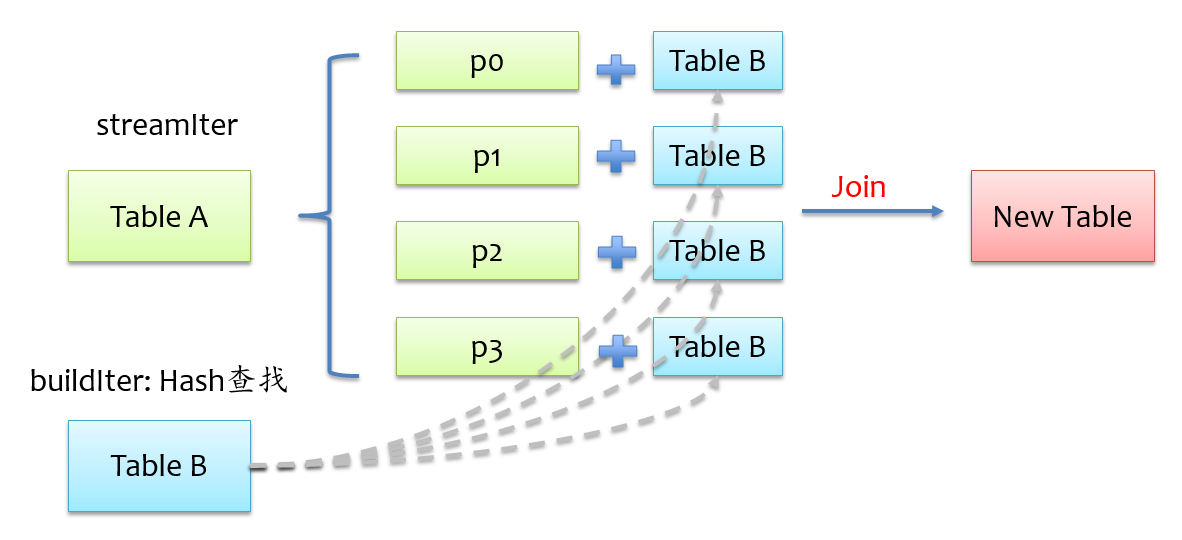
\includegraphics[width=1\textwidth]{Img/spark-sql-broadcast-join.png}
    \caption{Broadcast Join实现原理}
    \label{fig:broadcast-join}
\end{figure}

hash join是林外一种实现方式,具体过程如图\ref{fig:hash-join}所示。在shuffle read阶段不对记录排序,来自两个表具有相同key的记录会在同一个分区之中,在分区中不排序,将buildIter的记录放在hash表中,以便查找。这种情况下buildIter的记录放在hash表中,那么每个分区来自buildIter的记录不能太大,否则就无法存放在内存之中,默认情况下hash join是关闭的,需要满足以下四个条件才能使用hash join

\begin{itemize}
    \item buildIter的总体估计大小超过$spark.sql.autoBroadcastJoinThreshold$设定的值,不能满足broadcast join的条件
    \item 开始使用hash join的开关,$spark.sql.join.preferSortMergeJoin=false$
    \item 每个分区的平均大小不超过$spark.sql.autoBroadcastJoinThreshold$设定的值
    \item streamIter的大小是buildIter的三倍以上
\end{itemize}

可见使用hash join的条件非常苛刻,在大多数实际场景下,hash join和sort merge join的性能也不会有太大的区别,因为hash join也需要shuffle操作。

\begin{figure}[htbp]
    \centering
    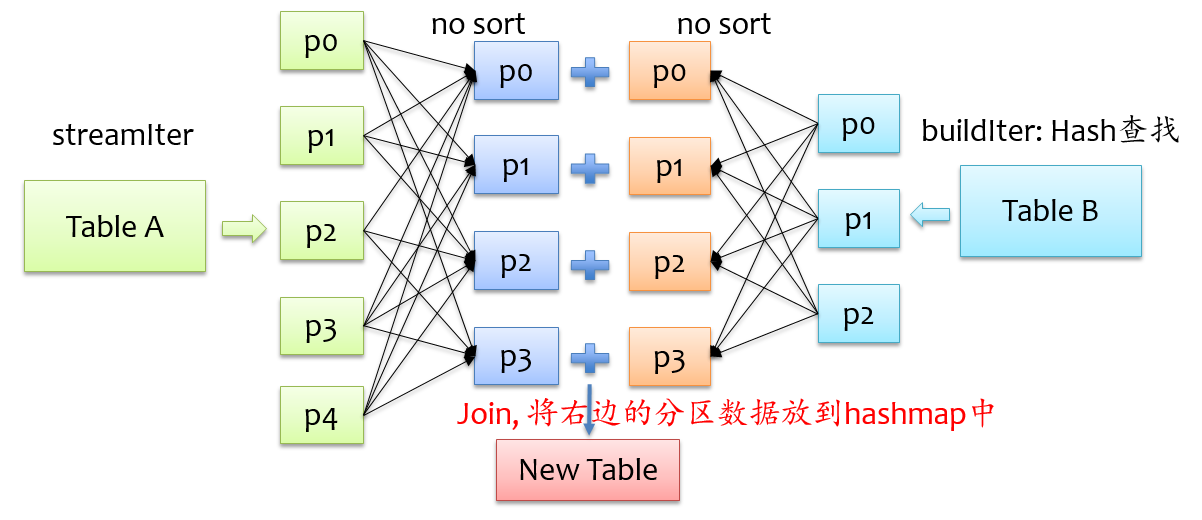
\includegraphics[width=1\textwidth]{Img/spark-sql-hash-join.png}
    \caption{hash Join实现原理}
    \label{fig:hash-join}
\end{figure}

下面再简单介绍不同join操作的实现方式。

inner join原理如图\ref{fig:inner-join},inner join需要找到左右表中满足join条件的记录,在buildIter查找记录时,如果右表不存在满足join条件的记录就跳过。

\begin{figure}[htbp]
    \centering
    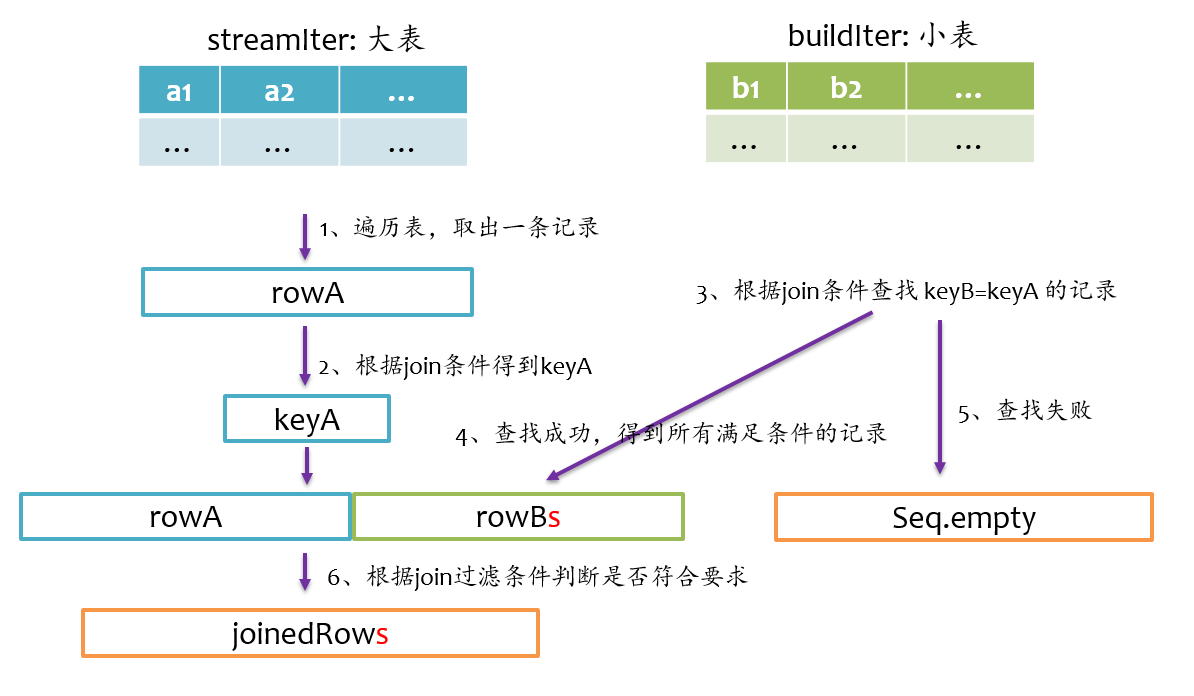
\includegraphics[width=1\textwidth]{Img/spark-sql-inner-join.png}
    \caption{inner Join实现原理}
    \label{fig:inner-join}
\end{figure}

left outer join的原理如图\ref{fig:leftouter-join}所示。left outer join以左表为准,根据join条件得到keyA,根据join条件在右表中查找满足匹配条件的记录,如果查找失败,则返回一个所有字段都为null的记录。如果查找成功就和左表组成一个新的记录。最后通过join的过滤条件过滤得到最后的结果。

\begin{figure}[htbp]
    \centering
    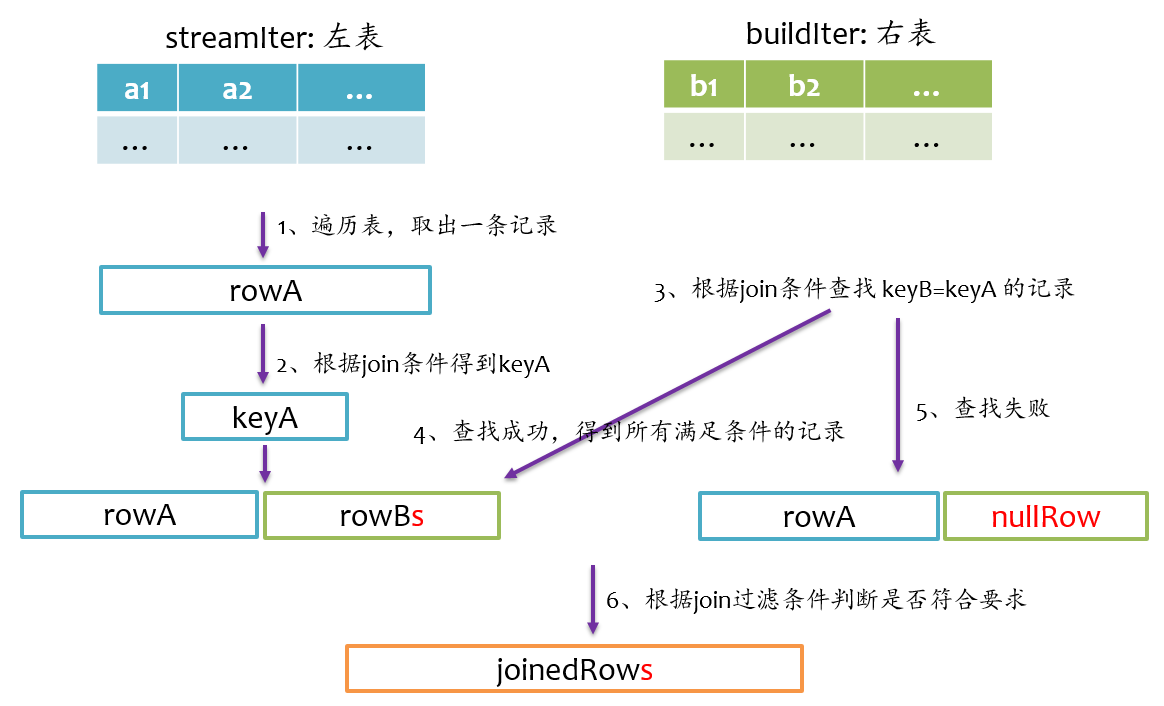
\includegraphics[width=1\textwidth]{Img/spark-sql-leftouter-join.png}
    \caption{left outer Join实现原理}
    \label{fig:leftouter-join}
\end{figure}

right outer join的原理如图\ref{fig:rightouter-join}所示。right outer join以右表为准,对于右表中的每一行记录,根据join条件计算得到keyB,然后根据keyB去坐标中查找条件相同的记录,如果查找失败会得到一个全为null的记录,如果查找成功就会和右表形成完整的记录。最终根据join的过滤条件得到最终的结果。

\begin{figure}[htbp]
    \centering
    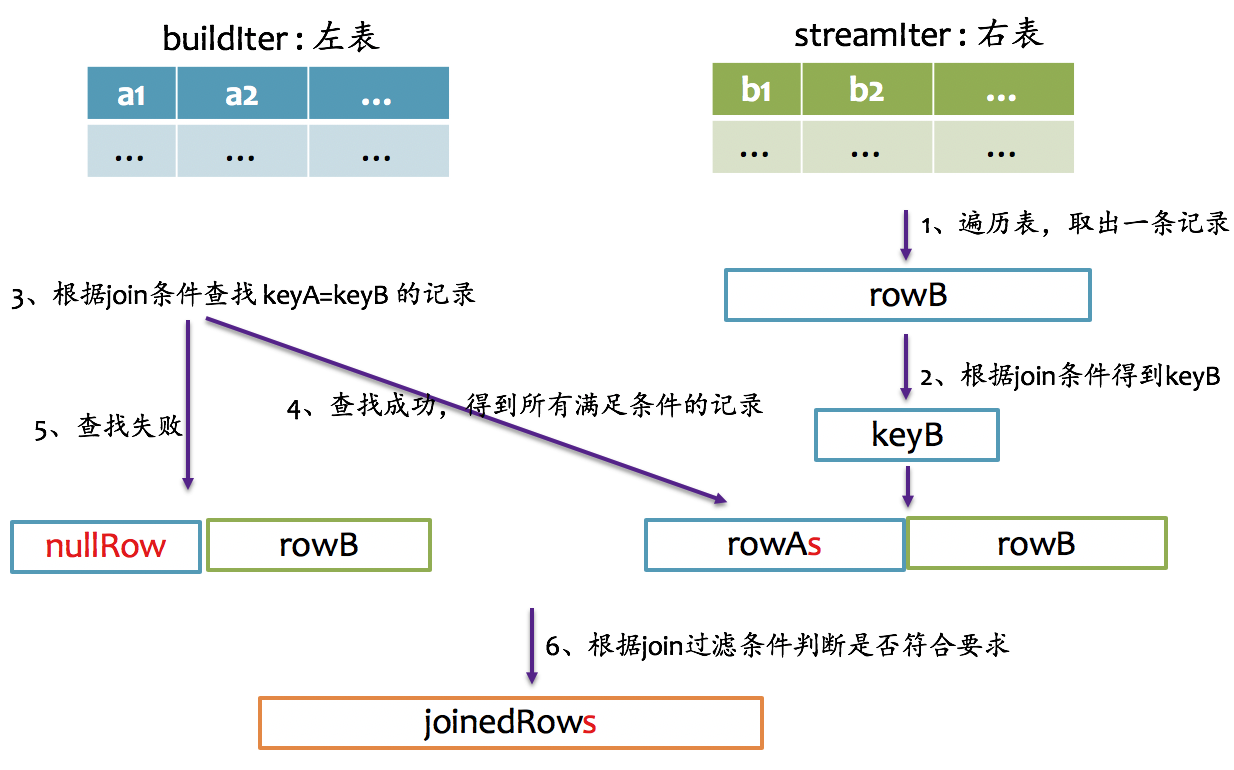
\includegraphics[width=1\textwidth]{Img/spark-sql-rightouter-join.png}
    \caption{right outer Join实现原理}
    \label{fig:rightouter-join}
\end{figure}


full outer join的原理如图\ref{fig:fullouter-join}所示,full outer join相对来说要更复杂一点,底层采用sort merge join实现。因为两个表已经排序,首先分别顺序从左表和右表中取出一条记录,比较key,如果key相同,则将rowA和rowB合并在一起,并且取出两表的下一条记录作为新的rowA和rowB。如果keyA<keyB,则说明右表中没有与左表rowA对应的记录,那么rowA指向下一条记录。如果keyA>keyB,说明左表中中没有与右表rowB对应的记录,那么rowB更新到右表的下一条记录,重复这个过程知道左右两张表的记录全部处理完成。

\begin{figure}[htbp]
    \centering
    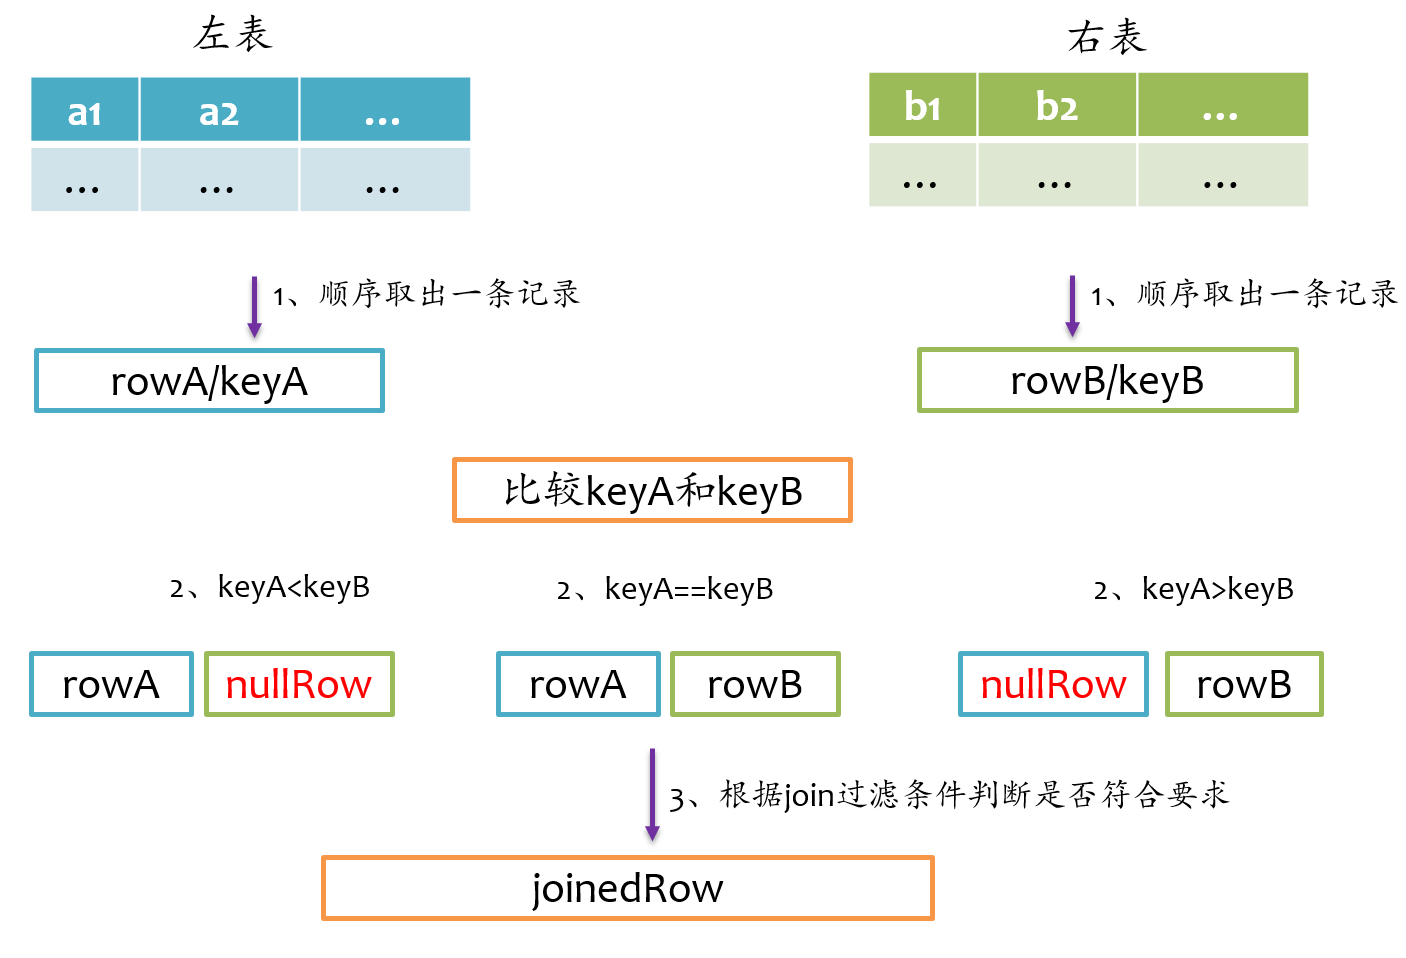
\includegraphics[width=1\textwidth]{Img/spark-sql-fullouter-join.png}
    \caption{full outer Join实现原理}
    \label{fig:fullouter-join}
\end{figure}

left semi join的原理如图\ref{fig:semi-join}所示。left semi join以左表为准,在右表中查找匹配的记录,如果查找成功就返回左边的记录。

\begin{figure}[htbp]
    \centering
    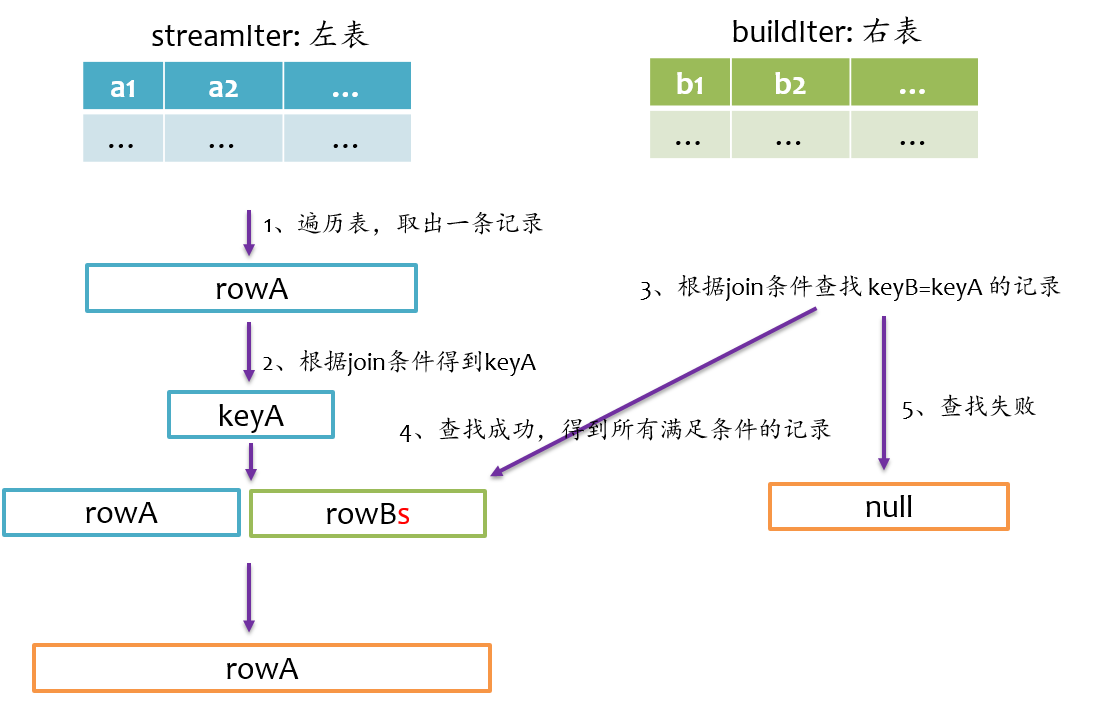
\includegraphics[width=1\textwidth]{Img/spark-sql-semi-join.png}
    \caption{semi Join实现原理}
    \label{fig:semi-join}
\end{figure}

left anti join的原理如图\ref{fig:anti-join}所示,以左表为准,在右表中查找匹配的记录,如果查找成功,就返回左边的记录。

\begin{figure}[htbp]
    \centering
    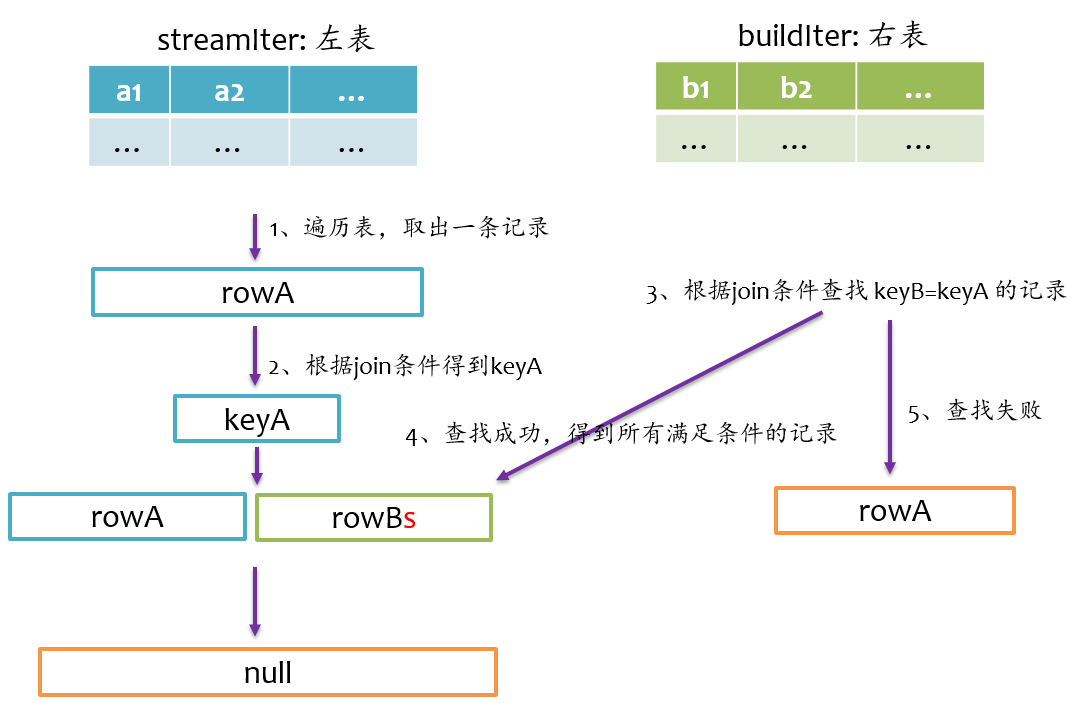
\includegraphics[width=1\textwidth]{Img/spark-sql-anti-join.png}
    \caption{anti Join实现原理}
    \label{fig:anti-join}
\end{figure}

\section{Spark内存管理模块分析}

Spark是一种基于内存的分布式计算框架,在计算的过程中通过将数据缓存在内存中加速计算过程。所以内存管理模块是Spark系统的核心模块。Spark内存管理机制在JVM虚拟内存管理的基础上对Executor模块拥有的内存进行了进一步的分配管理。也支持在Executor外的系统内存中直接开辟内存空间用于存储计算过程中产生的大量数据。通过使用对外内存,可以减少内存空间不足导致的垃圾回收以及内存不足错误。

Spark框架执行过程中内存管理模块会申请JVM内存,申请的大小由配置参数决定。内存管理模块会将内存分为四个部分。Storage Memory,Execution Memory,User Memory,Reserved Memory。四部分内存有不同的用途。

\begin{enumerate}
    \item Storage Memory 用于缓存中间数据。比如对于一份数据data1,在之后计算过程中需要重复使用。就可以调用data1.cache接口将数据缓存在Storage Memory区域。在之后计算过程中框架就可以直接从Storage Memory区域读取数据。具体来说,调用cache接口并不会立刻将数据写入缓存之中,而只是设置了STORAGE\_LEVEL这个标记为MEMORY\_ONLY。后续在框架执行的过程中,当data1被计算得到时,框架会检查STORAGE\_LEVEL这个标记,发现为MEMORY\_LEVEL后会通过memory maneger将其存入Storage Memory之中。这个过程并不会造成内存拷贝复制。memory manager只是将指向数据的引用从Execution Memory移到Storage Memory之中,并更新两个内存区域内存总量。
    
    \item Execution Memory 用于框架计算过程。在计算过程中比如对于Shuffle操作,需要在内存中缓存一部分数据,再一次性写入文件系统之中,从而避免频繁磁盘IO导致的延迟。在计算的过程中数据也都存放在Executor Memory之中。比如上面所说的data1,在计算过程中一直使用Execution Memory。在计算结束之后根据STORAGE\_LEVEL,如果为MEMORY\_ONLY就会移到Storage Memory之中。
    
    \item User Memory 为应用程序使用的内存空间。应用程序创建的各种和Spark框架无关的对象都会存在User Memory之中。
    
    \item Reserved Memory 的目的是避免发生OOM(Out of Memory)错误。OOM问题的根本原因是框架的内存管理和底层JVM的内存管理是完全隔离的。框架只是简单的记录内存的使用量,但是记录的内存使用量和实际的内存使用量并不是一一对应的。首先User Memory的内存是框架无法准确感知的。其次Storage Memory区域的内存也是不准确的,比如Storage Memory区域缓存有一份数据data1。之后应用程序调用data1.uncache接口将data1数据从内存中清除。框架所做的工作是在缓存管理模块中将data1的引用释放,并且将data1的内存总量加到Storage Memory的空闲内存之中,表示这些内存空间空闲。但是此时data1实际占用的JVM内存并没有被释放,实际内存的释放完全依赖于JVM虚拟机的垃圾回收机制,如果此时框架有新的内存申请请求,就有很大可能让框架实际使用内存超过向JVM申请的资源,导致OOM错误。所以需要保留一段空闲内存,避免这种OOM的出现。但是这种方法也有一些缺点,首先它并不能完全消除OOM错误,只要多申请的内存超过Reserved Memory的大小,还是会导致出错。另一方面Reserved Memory所占用的内存资源完全被浪费了,造成内存资源利用率下降。
\end{enumerate}

目前内存管理模块有两种模式,默认模式和Legacy模式。默认模式Storage Memory和Execution Memory是共享内存空间的。Legacy模式下Storage Memory和Execution Memory是隔离的,通过配置文件可以配置两者的大小。

\subsection{弹性分布式数据集RDD}

\begin{figure}[htbp]
    \centering
    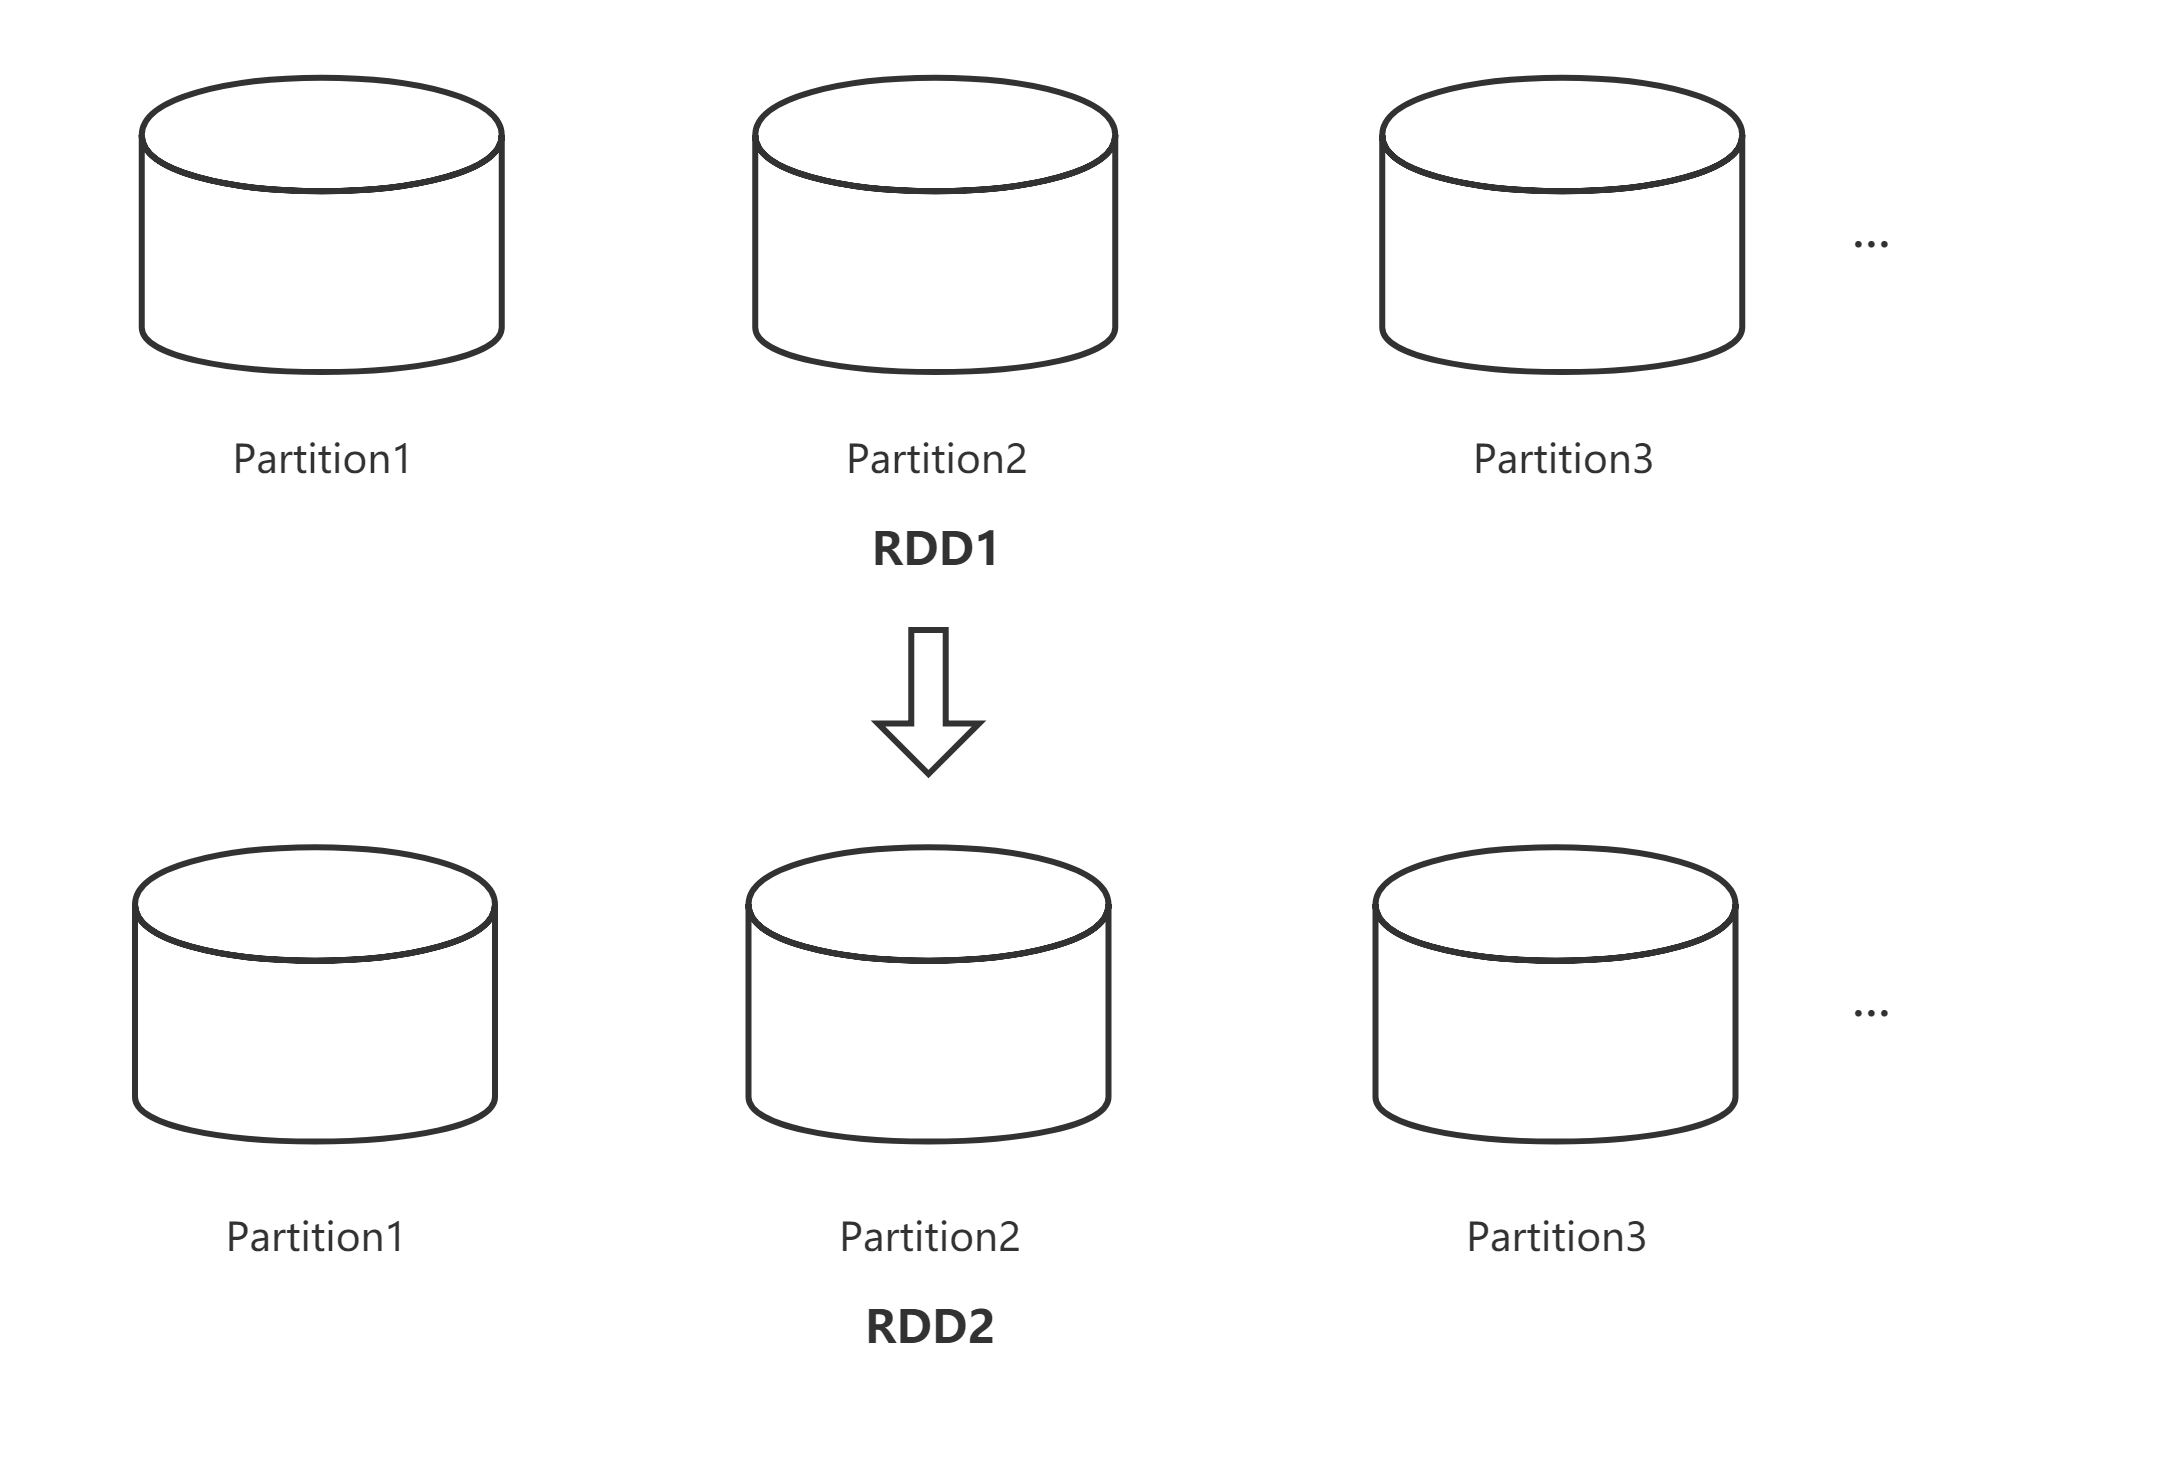
\includegraphics[width=1\textwidth]{Img/RDD示意图.png}
    \caption{只读弹性分布式数据集RDD}
    \label{fig:rdd}
\end{figure}

弹性分布式数据集(Resilient Distributed Datasets)是Spark框架的核型概念。RDD是指一种可并行可操作的只读数据集合。RDD利用了Scala语言的特性,Scala将数据分为可变数据variable和不可变数据value。RDD中的数据被设置成不可变数据,所以在创建之后就不能再改变了,因为是不可变数据,所以很适合并行处理。RDD数据有丰富的操作,操作也分为两类,transform和action。transform操作是将一个RDD转化为另一个RDD。因为对于用户来说RDD无法直接展示,所以框架也不会立即计算。action操作是计算出一个具体的结果,比如求和,求平均数等操作。因为需要计算具体的结果,所以框架只有遇到action操作才会具体计算。RDD数据之间的操作相当于作业DAG图中的边。RDD相当于DAG图中的点。Spark框架通过DAG图的拓扑来解决容错的问题。比如data1是由data2和data3计算得到的。在DAG图中就有data1指向data2和data3的两条边。在计算data1的过程中框架会沿着这两天边检查data2和data3的状态,如果data2和data3保存在内存之中,框架会直接进行计算,如果保存在磁盘之中,框架会从磁盘中将数据加载到内存之中进行计算。如果数据完全丢失了,框架就会重新计算RDD数据。

\begin{table}
 \centering
 \small
 \caption{transformation算子}
 \label{tab:transformation}
 \resizebox{\columnwidth}{!}{%
 \begin{tabular}{lccccccccl}
  \toprule
  算子名称 & 算子操作 \\
  \midrule
  $map(f: T \Rightarrow  U)$ & $RDD[T] \Rightarrow RDD[U]$ \\
  $filter(f : T \Rightarrow Bool)$ & $ RDD[T] \Rightarrow RDD[U] $ \\
  $flatMap(f : T \Rightarrow Seq[U]) $ & $ RDD[T] \Rightarrow RDD[U] $ \\
  $sample(fraction : Float)$ & $RDD[T] \Rightarrow RDD[T]$ \\
  $groupByKey()$ & $RDD[k, v] \Rightarrow RDD[K, Seq[V]]$ \\
  $reduceByKey(f : (V, V) \Rightarrow V)$ & $RDD[K,V] \Rightarrow RDD[K,V]$ \\
  $union()$ & $(RDD[T], RDD[T]) \Rightarrow RDD[T]$ \\
  $join()$ & $(RDD[K,V], RDD[K,W]) \Rightarrow RDD[K, (V, W)]$ \\
  $cogroup()$ & $(RDD[K,V], RDD[K,W]) \Rightarrow RDD[K, (Seq[V], Seq[W])]$ \\
  $crossProduct()$ & $(RDD[T], RDD[U]) \Rightarrow RDD[(T,U)]$ \\
  $mapValues(f : V \Rightarrow W)$ & $RDD[K,V] \Rightarrow RDD[K,W]$ \\
  $sort(c:Comparator[K])$ & $RDD[K,V] \Rightarrow RDD[K,V]$ \\
  $partitionBy(p : Partitioner[K])$ & $RDD[K,V] \Rightarrow RDD[K,V]$ \\
  \bottomrule
 \end{tabular}}
\end{table}

\begin{table}
 \centering
 \small
 \caption{action算子}
 \label{tab:action}
 \resizebox{\columnwidth}{!}{%
 \begin{tabular}{lccccccccl}
  \toprule
  算子名称 & 算子操作 \\
  \midrule
  $count()$ & $RDD[T] \Rightarrow Long$\\
  $collect()$ & $RDD[T] \Rightarrow Seq[T]$\\
  $reduce(f : (T,T) \Rightarrow T)$ & $RDD[T] \Rightarrow T$\\
  $lookup(k, K)$ & $RDD[K,V] \Rightarrow Seq[V]$\\
  $save(path:String)$ & 将RDD数据存储到存储系统\\
  \bottomrule
 \end{tabular}}
\end{table}

\begin{figure}[htbp]
    \centering
    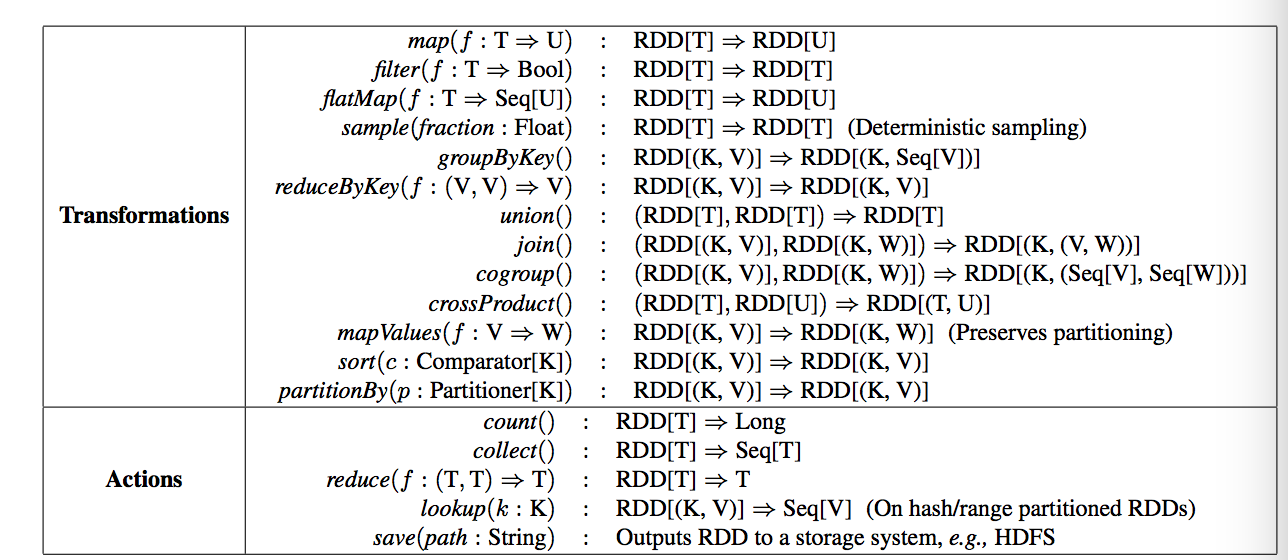
\includegraphics[width=1\textwidth]{Img/rdd-transformations-actions.png}
    \caption{transformation和action算子}
    \label{fig:rdd-transformation-action}
\end{figure}

\begin{figure}[htbp]
    \centering
    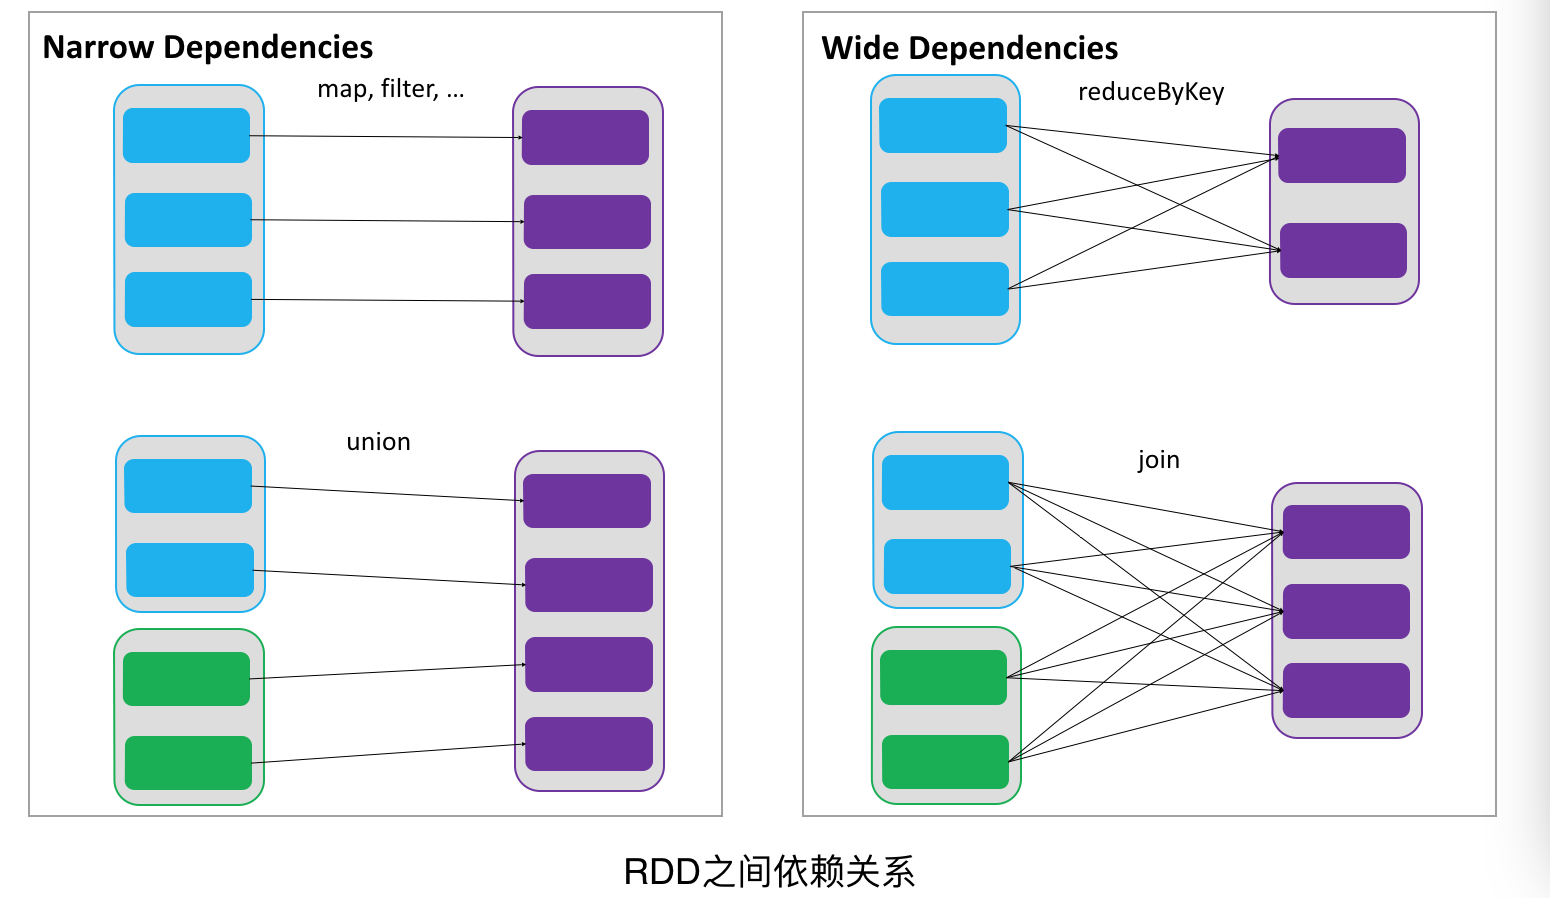
\includegraphics[width=1\textwidth]{Img/rdd-dependency.png}
    \caption{宽依赖与窄依赖}
    \label{fig:rdd-dependency}
\end{figure}


\begin{figure}[htbp]
    \centering
    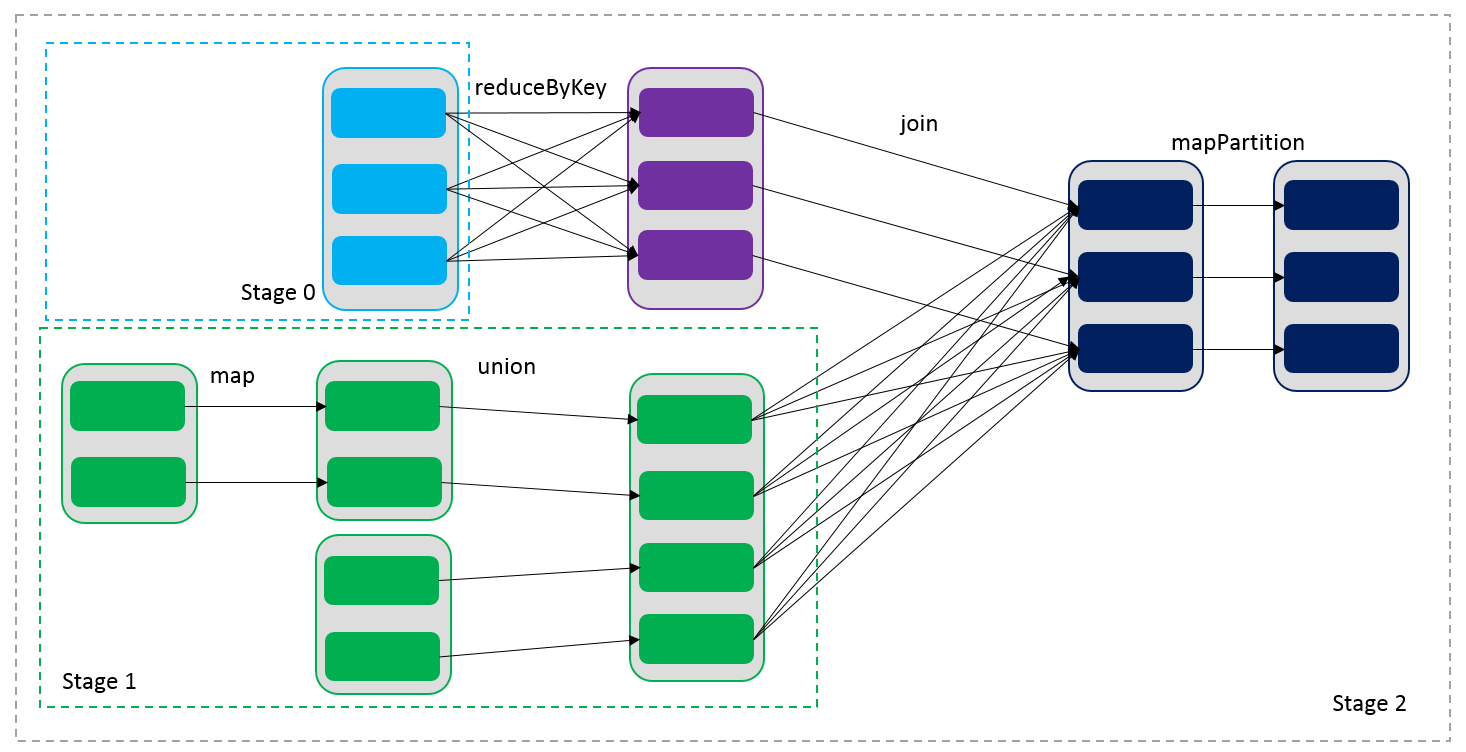
\includegraphics[width=1\textwidth]{Img/rdd-dag.png}
    \caption{stage划分示意图}
    \label{fig:rdd-dag-stage}
\end{figure}

RDD之间的关系还可以进一步分类。如果转化操作的逻辑可以转化为窄依赖和宽依赖两种。窄依赖是指父RDD的每个分区只被一个子RDD的分区使用,这种依赖关系下,父子RDD之间数据交换无需进行shuffle操作,父RDD只需将数据发送给子RDD即可。宽依赖是指父RDD的分区数据会被多个子RDD的分区使用,也就是说父RDD输出的数据会被多个子RDD使用,这就需要在父子之间进行Shuffle交换数据,宽窄依赖主要用于作业调度执行。框架在执行过程中遇到一个action操作就会提交一个job,在job调度执行期间,DAGScheduler会把所有宽依赖所在的边切分,将整个DAG计算图切分成多个子图,每个子图称为一个stage,DAGScheduler将stage发送给TaskScheduler调度执行每一个任务。

\subsection{缓存数据管理模块}

缓存存储模块主要包含如下两个部分,RDD缓存和Shuffle数据缓存。缓存模块的主要工作是管理RDD缓存,包括内存和磁盘的缓存。Shuffle中间数据的管理也是有缓存管理模块完成。存储模块中管理着多种不同的数据,包括RDD数据块、Shuffle数据块、广播变量数据块、任务返回数据块、流式数据块。RDD数据块用于标记缓存的RDD数据。Shuffle数据块用于标识缓存的Shuffle数据。广播变量数据块用于标识广播变量。任务返回数据块用于标识任务赶回结果数据。流式数据块在Spark Streaming中用于标记收到的流式数据。

BlockManager模块用于管理各种缓存数据。RDD分区数据,Shuffle数据,broadcast数据都由BlockManager管理。BlockManager是一个主从结构。在Driver节点和Executor节点都有BlockManager,Executor节点的BlockManager会将block数据块的数据都发送给Driver节点的BlockManager统一管理。BlockManager对外提供get和set接口,可以将数据存储在内存、磁盘或者堆外内存。

Driver初始化的时候会创建BlockManager的时候会创建一个BlockManagerMasterEndpoint,之后Driver会将BlockManagerMasterEndpoint发送给Executor节点,Executor节点收到后会创建自己的BlockManager,并且通过BlockManagerMasterEndpoint向Driver节点上报注册信息。


BlockManager模块有MemoryStore和DiskStore两个模块用以存储block。DiskStore使用磁盘存储缓存数据,DiskStore中有一个成员DiskStoreManager,它的主要作用是管理逻辑block和物理block之间的映射关系,DiskStore中的block对应文件系统中的一个文件。DiskStore接收到缓存请求的时候会根据规则创建一个文件并将文件写入文件之中。MemoryStore使用Executor的JVM堆内存存储数据。MemoryStore中维护了一个LinkedHashMap来管理所有的block,Scala语言的LinkedHashMap底层通过链表存储数据,会将访问的数据移到链表头部。所以LinkedHashMap是具有LRU的特性的。MemoryStore模块就是巧妙地利用LinkedHashMap实现LRU替换策略的。

\begin{figure}[htbp]
    \centering
    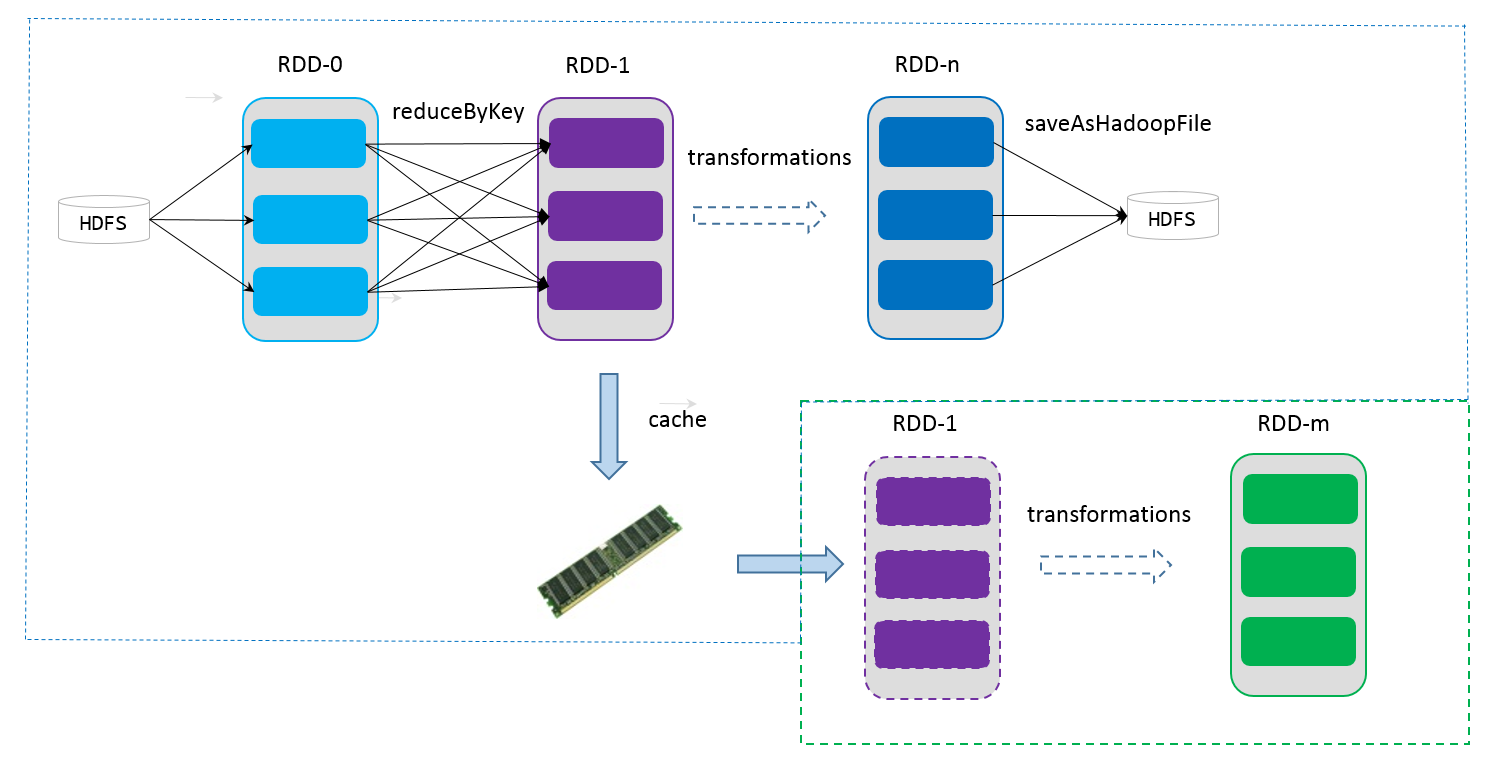
\includegraphics[width=1\textwidth]{Img/rdd-cache.png}
    \caption{数据缓存示意图}
    \label{fig:rdd-cache}
\end{figure}

\subsection{Shuffle原理解析}

在传统Hadoop系统之中Shuffle是连接Map操作和Reduce操作的桥梁,在Spark之中Shuffle操作使用场景更多。Shuffle操作将map的输出对应到reduce的输入中,Shuffle操作涉及到序列化和反序列化、跨节点网络通信IO以及磁盘读写IO等。所以说Shuffle操作是整个应用程序运行过程中非常重要的一个阶段。

Spark的Shuffle实现大致如图\ref{fig:shuffle-overview}所示,对于一个DAG计算图,以Shuffle操作为界,划分stage,上游stage为map阶段,下游stage为reduce阶段。map阶段的每一个任务计算得到一个分区,将分区数据分成多份,每一份发送给下游stage对应的分区,并且将临时结果写入磁盘,这个过程叫做shuffle write;下游stage为reduce task,每个reduce task通过网络拉去上游stage中所有map task的指定分区结果数据,该过程叫做shuffle read,最后完成整个计算过程。这里举一个例子说明,例如上游stage有M个map task,下游stage有N个reduce task,那么上游stage的每个map task都会将输出数据分为N份。下游stage的每个reduce task会从上游拉去M个数据。整个Shuffle过程会产生$M \times N$个临时小文件,每个小文件都要写入磁盘,导致大量碎片写磁盘操作,每个小文件也会通过网络传输给下游节点,造成大量网络传输。

\begin{figure}[htbp]
    \centering
    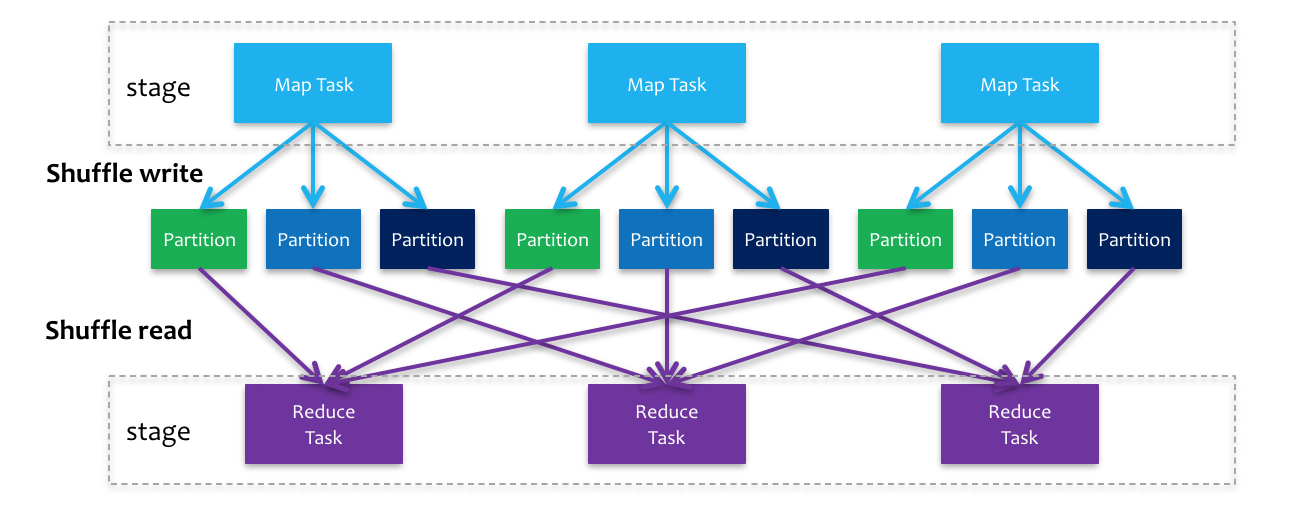
\includegraphics[width=1\textwidth]{Img/spark-shuffle-overview.png}
    \caption{Hash Shuffle V1原理图}
    \label{fig:shuffle-overview}
\end{figure}

为了解决这些问题,Spark进行了一系列的优化,如图\ref{fig:shuffle-v2}为了减少临时小文件的数量,Spark使用将map task输出的小文件合并到同一个文件,这样下游的reduce task只需要一次性从上游拉去一个文件,大大减少了碎片文件传输的问题。但是假如下游stage的分区数量N很大,还是会在每个Executor节点生成N个文件。如果一个Executor上有K个task,会有$K \times N$个file writer,总体上来没有从根本上解决问题。


\begin{figure}[htbp]
    \centering
    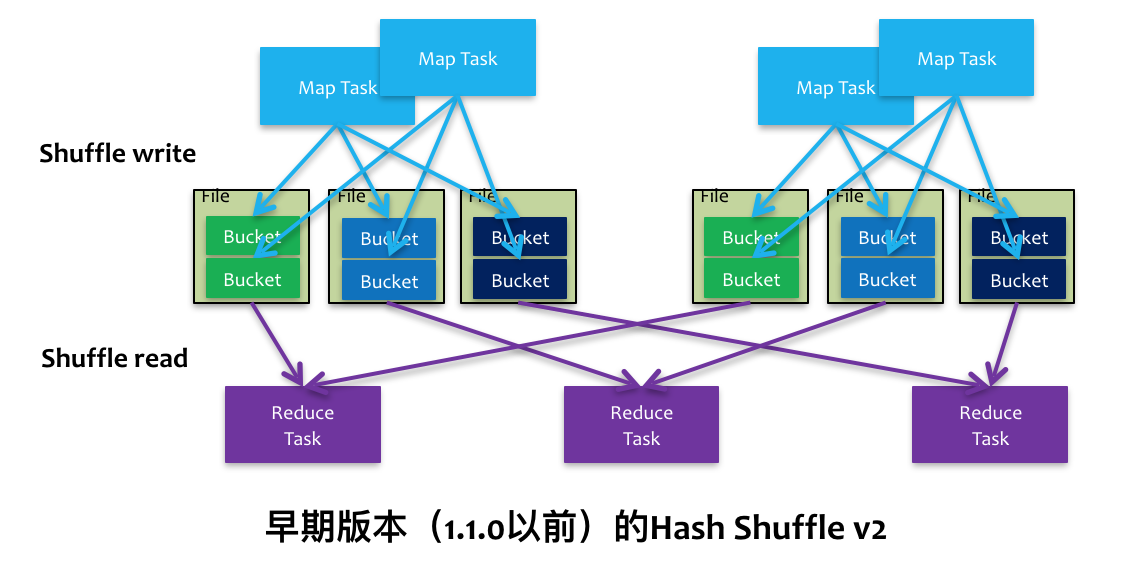
\includegraphics[width=1\textwidth]{Img/spark-shuffle-v2.png}
    \caption{Hash Shuffle V2原理图}
    \label{fig:shuffle-v2}
\end{figure}


针对Hash Shuffle存在的问题,Spark引入了Sort Shuffle。在map阶段的shuffle write操作,会按照paitition id以及key对记录进行排序,将所有partition的数据写入同一个文件中,该文件中的数据会按照partition id排序存放,每个partition内部按照key进行排序存放,map task会按照顺序写每个partition的数据,并通过索引文件记录每个partition的大小和偏移量。这样每个map task只需要开启两个file writer,一个写数据,一个写索引,大大减轻了Hash Shuffle存在的大量file writer的问题,如果一个executor有K个task,最多一次性会开启$K \times 2$个文件描述符。在reduce阶段,reduce task拉去数据做combine操作时不再使用HashMap,而是采用ExternalAppendOnlyMap,该数据结构在做combine操作时,如果内存不足会将数据写入磁盘之中,这就保证了系统的鲁棒性。避免了数据量比较大情况下OOM的问题。


\begin{figure}[htbp]
    \centering
    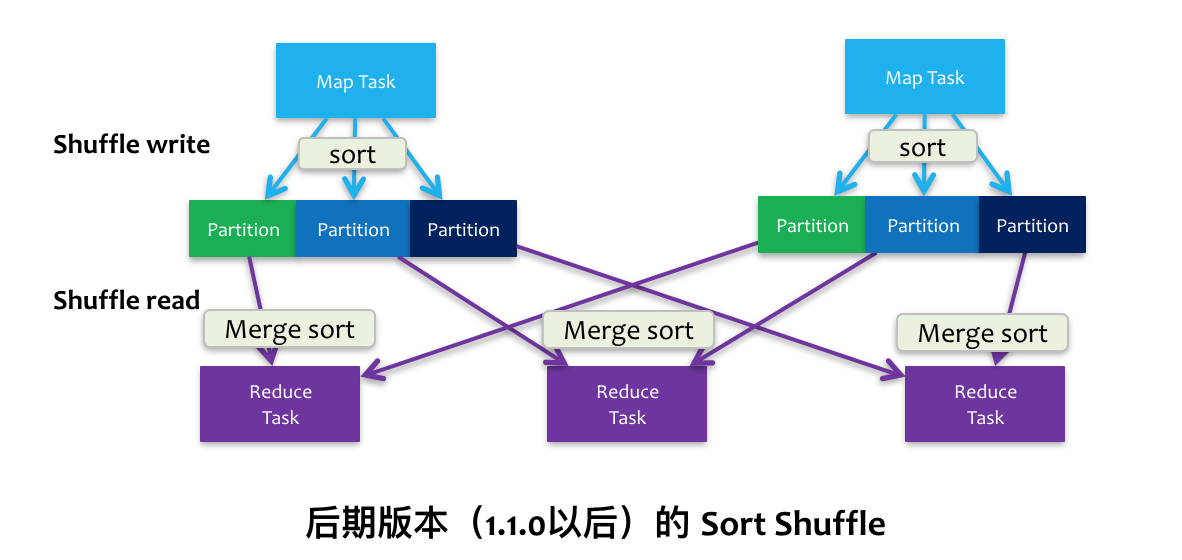
\includegraphics[width=1\textwidth]{Img/sort-shuffle.png}
    \caption{Sort Shuffle原理图}
    \label{fig:sort-shuffle}
\end{figure}



\section{应用举例}

这里介绍一个简单的spark应用程序实例WordCount,统计一个数据集中每个单词出现的次数,首先将从hdfs中加载数据得到原始RDD-0,其中每条记录为数据中的一行句子,经过一个flatMap操作,将一行句子切分为多个独立的词,得到RDD-1,再通过map操作将每个词映射为key-value形式,其中key为词本身,value为初始计数值1,得到RDD-2,将RDD-2中的所有记录归并,统计每个词的计数,得到RDD-3,最后将其保存到hdfs。这个应用程序转化为DAG图结构如图\ref{fig:word-count}所示。

\begin{lstlisting}[language=Scala]
import org.apache.spark._
import SparkContext._

object WordCount {
  def main(args: Array[String]) {
    if (args.length < 2) {
      System.err.println("Usage: WordCount <inputfile> <outputfile>");
      System.exit(1);
    }
    val conf = new SparkConf().setAppName("WordCount")
    val sc = new SparkContext(conf)
    val result = sc.textFile(args(0))
                   .flatMap(line => line.split(" "))
                   .map(word => (word, 1))
                   .reduceByKey(_ + _)
    result.saveAsTextFile(args(1))
  }
}
\end{lstlisting}

\begin{figure}[htbp]
    \centering
    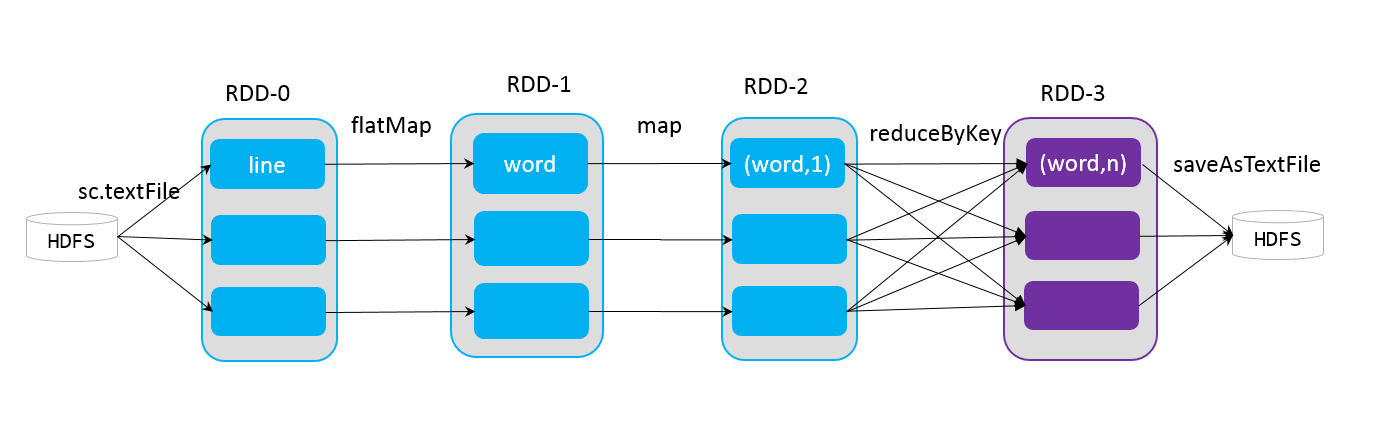
\includegraphics[width=1\textwidth]{Img/spark-wordcount.png}
    \caption{wordCount程序DAG图}
    \label{fig:word-count}
\end{figure}

\section{本章总结}

本章全面的介绍了Spark框架。第一部分介绍了Spark系统的概况。第二部分介绍了Spark系统的核型概念和整体架构。第三部分详细介绍了Spark的核型调度执行模块,包括从DAG到底层Task调度的所有流程。第四部分详细介绍了内存管理模块,包括Spark的核心概念分布式弹性数据集RDD、缓存数据管理模块。本章对框架原理的深入解析为下文自动缓存模块以及缓存管理优化奠定了基础。





\chapter{Spark自动缓存模块设计与实现}\label{chap:auto-cache}

本章首先对Spark缓存管理机制进行了深入的分析,从而引出了自动缓存的需求。之后详细阐述了自动缓存模块的设计与实现,最后介绍了测试数据集SparkBench,并对自动缓存模块进行了一系列的测试。

\section{Spark相关模块现状分析}
Spark框架相对于Hadoop的核心改进是添加了缓存管理模块。通过将计算过程中的中间数据缓存在内存中可以极大的加速计算过程。尤其对于机器学习和图计算等迭代式计算有上百倍的加速效果。这是因为这种迭代式计算需要多次重复访问中间数据,就非常能体现Spark框架的优势。

\subsection{缓存模块底层原理}
Spark应用在执行过程中会将应用程序解析成DAG图,然后根据DAG的拓扑排序顺序执行DAG图中的每一个操作。一个RDD数据被计算得到之后,会存放在Execution Memory区域。如果没有立即被使用使用到就会从Execution Memory区域被删除。Spark框架给应用程序员提供了cache接口,cache接口会将RDD对象的STORAGE\_LEVEL字段标记为MEMORY\_ONLY。标记之后Spark框架并不会立即缓存数据,而是在RDD分区数据计算完成时查看STORAGE\_LEVEL标记。根据不同的标记将数据缓存到不同的位置,常见的标记有以下几种,MEMORY\_ONLY,DISK\_ONLY,MEMORY\_AND\_DISK。如果标记为MEMORY\_ONLY框架就会将数据缓存到内存之中,具体过程是将RDD的应用发送给BlockManager对象的MemoryStore模块。MemoryStore模块会保存RDD模块的引用。这样就能将RDD对象长时间保存在内存中。从缓存管理模块的逻辑视图角度来看cache接口调用是将RDD对象从Execution Memory区域移到了Storage Memory区域。如果STORAGE\_LEVEL标记为DISK\_ONLY。框架会将RDD对象的引用发送给BlockManager的DiskStore模块。DiskStore模块在HDFS或者其他文件系统上创建一个文件,将RDD对象写入文件之中。并且保存文件的路径。这就是缓存管理模块的核心过程。

当要使用到一个RDD数据时,框架会从BlockManager模块查看数据是否存在缓存数据。此时有两种情况,如果缓存数据存放在磁盘之中框架会将数据读取加载到内存的Execution Memory区域。如果是缓存在内存之中就可以直接进行计算。

在分析了缓存模块的核心原理之后还有一个重要的问题,就是缓存决策是如何实现的。目前Spark应用的缓存决策全都由编程人员在开发的过程中手动指定。这存在着几个问题。第一,编程人员可能会做出不正确的缓存决定,缓存了无用的数据,这会导致内存被浪费,降低了系统内存资源的使用效率。第二,编程人员可能没有缓存重要数据,导致在计算的过程中重复计算重要数据,对应用程序的执行时间造成巨大的影响。第三,这种编程模式对Spark应用编程人员提出了比较高的要求,编程人员必须熟悉Spark框架的核心原理,还要熟悉Spark提供的众多算子的底层实现,在此基础上还需要在编程的过程中选择合适的数据进行缓存,在Spark应用程序规模变大之后就会对编程人员造成比较大的负担。

\subsection{自适应执行框架原理}
同时还需要考虑Spark框架最新的动态执行新特性。Spark框架本身是在不断发展之中,Spark这类并行数据处理系统存在着一些问题,下面三个问题对性能影响比较突出:

\begin{enumerate}
    \item shuffle partition 个数,比如spark的shuffle partition个数默认值为200。可以通过参数配置,这个参数决定了reduce阶段任务的数量,对整个查询的性能有很大的影响。假设一个查询运行前申请E个Executor,每个Executor包含C个core(并发执行线程数),那么该作业在运行时可以并行执行的作业个数就为$E\times C$个,也可以说该作业的并发数为$E\times C$个。假设shuffle partition个数为P,处理map stage的任务数和原始数据的文件数量和大小有关,后续的每个reduce stage的任务数量都为P。由于Spark作业调度是抢占式的,$E\times C$个作业会抢占执行P个任务,直至所有任务完成,就会进入下一个stage。在这个过程中,任务执行时间会过长,导致整个stage执行时间变长,另一方面,$E\times C$个执行单元大部分都处于空闲状态,导致整体资源利用率急剧下降。所以shuffle partition个数的设置就对性能有着很大的影响,在实际运行场景下,作业执行之前很难设置shuffle partion个数。
    \item 最佳执行计划,Spark SQL会将应用程序翻译成逻辑计划,然后经历一系列的优化,最后确定一个物理执行计划。最终选择的物理执行计划对性能有很大的影响。如果选择最佳的执行计划是Spark SQL的Catalyst优化器的核心工作。Catalyst早期主要是基于规则的优化器(RBO,Rule Based Optimizer),在Spark2.2中加入了基于代价的优化(CBO, Cost Based Optimizer)。也有一些工作实现了根据历史记录的优化(HBO,History Based Optimizer)。这些优化器统一的特点是在作业执行之前完全确定物理执行计划,一旦确定之后就不再改变。然而实际作业往往在事先无法完全预料。如图\ref{fig:wrong-sort-join}所示。其中一张表的大小仅为600KB,然后Spark申城的物理执行计划依旧使用了sortMergeJoin。这种场景明显使用BroadcastJoin更加合理。
    \item 数据倾斜问题。数据倾斜是常见的导致SparkSQL性能变差的问题。数据倾斜是指某一个partition的数据量远远大于其他partition的数据。导致个别任务的运行时间远远大于其他任务,因此拖累了整个作业的运行时间。在实际作业中,数据倾斜问题很常见,这是因为join key对应的hash值分布不均匀。在极端情况下,hash结果分布非常不均匀,导致大量数据被分到同一个partition二导致严重数据倾斜。如图\ref{tab:data-qinxie}所示,大部分任务在两秒内就完成了,但是最慢的任务却花了4分钟,这就是因为发生了数据倾斜问题,他处理的数据是其他任务的数倍。最终虽然大部分很快就运行结束,因为数据倾斜问题,整个作业的执行时间也被极大地影响了。

\end{enumerate}

\begin{figure}
    \centering
    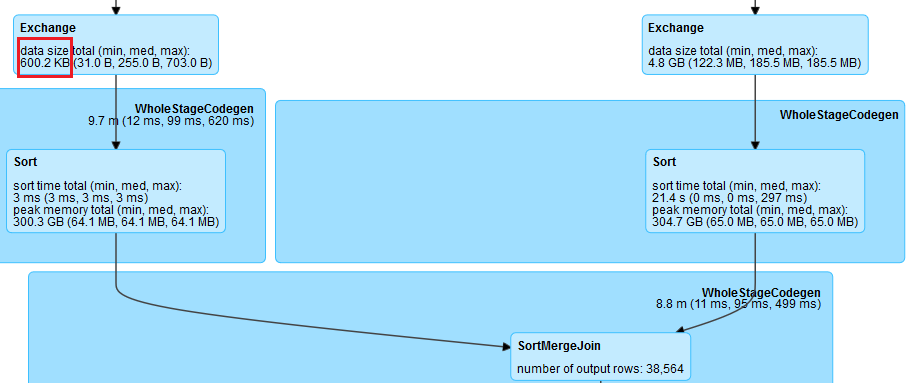
\includegraphics[width=0.99\textwidth]{Img/wrong-sort-join.png}
    \caption{不合理的物理执行计划}
    \label{fig:wrong-sort-join}
\end{figure}


\begin{table}
 \centering
 \small
 \caption{SparkBenck支持的负载}
 \label{tab:data-qinxie}
 \resizebox{\columnwidth}{!}{%
 \begin{tabular}{lccccccccl}
  \toprule
  Metric & Min & 25th percentile & Median & 75th percentile & Max \\
  \midrule
  Duration & 15ms & 2s  & 3s  & 5s & 4min \\
  Scheduler Delay & 0ms & 2ms & 2ms & 3ms & 1s \\
  Task Deserialization Time & 3ms & 5ms & 6ms & 7ms & 0.4s \\
  GC Time & 0ms & 0ms & 0.2s & 0.3s & 35s \\
  Result Serialization Time & 0ms & 0ms & 0ms & 0ms & 3ms \\
  Getting Result Time & 0ms & 0ms & 0ms & 0ms & 0ms \\
  Peak Execution Memory & 0B & 0B & 0B & 0B & 0B \\
  Shuffle Read Blocked Time & 0ms & 44ms & 0.2s & 0.6s & 31s \\
  Shuffle Read Size/Records & 0B/0 & 3.5MB/374415 & 4.0MB/747052 & 6.9MB/1783859 & 172.8MB/283732661 \\
  Shuffle Write Size/Records & 0B/0 & 109B/3 & 132B/4 & 158B/6 & 262B/13 \\
  Shuffle spill(memory) & 0B & 0B & 0B & 0B & 13.3GB \\
  Shuffle Write(disk) & 0B & 0B & 0B & 0B & 68.2MB \\
  \bottomrule
 \end{tabular}}
\end{table}

对于这些问题,Spark设计实现了一套自适应执行框架。自适应执行框架的思路是在执行计划中划分好stage,然后按照stage提交执行,在运行过程中收集当前stage的统计信息,通过运行时信息来优化下一个stage的物理执行计划,然后提交后续的stage。在运行过程中,Spark动态执行框架会根据运行情况动态设置下游Reducer个数、动态调整执行计划、动态处理数据倾斜问题。

\section{自动缓存模块}

\subsection{自动缓存模块设计}
通过上文对Spark相关模块的详细分析后,本文设计了一种改进的自动缓存模块。需要实现自动缓存的功能,就需要能够判断在整个作业计算过程中哪些数据会被重复使用,对于需要重复使用的RDD数据,应该将其缓存在缓存之中,这样在之后的计算过程中,Spark框架就可以直接使用已经缓存的数据进行计算,从而能够加速计算过程。

针对Spark底层实现原理来分析,Spark会将应用程序转化为一个DAG图,这里使用$G(V, E)$来表示DAG。DAG图中的节点$V$是RDD数据,DAG图中的边$E$为RDD数据之间的转化关系,分为transformation和action两种。根据action操作,Spark框架会将整个DAG切分成多个作业,这里用$J={j_1, j_2,...,j_m }$表示所有作业。对于每个作业$j_i$,Spark框架会根据宽依赖将作业分为多个stage。如果$RDD_i$通过操作转化为$RDD_j$,其中存在一条边$(i, j)\in E$,那么$RDD_i$就称为$RDD_j$的父节点。对于$RDD_v$来说,它的所有父节点记为$anc(v)$。它的所有后继节点记为$dsc(v)$。

根据对Spark底层DAG图结构进行分析之后发现需要得到应用对应的DAG图,只要得到了DAG图,然后对DAG图进行分析就可以得到重复使用的RDD数据,在DAG图中,对于$RDD_v$, $dsc(v)$的大小就是会被重复使用的次数。在程序运行之前是很难得到DAG图结构,所以可以使用少量输入数据运行整个应用程序,然后记录DAG图结构。之后使用全量输入数据再次运行整个程序,这样就可以在第二次执行过程中缓存需要重复使用的数据。

在上文介绍了Spark的动态执行功能。动态执行功能会在执行过程中根据stage的运行时数据优化调整接下来的物理执行计划,所以当Spark调整执行计划时,自动缓存模块也需要同步更新修改DAG图结构,这样就可以保持正确的DAG图结构。

\subsection{自动缓存模块实现}
Spark应用程序都会创建一个SparkContext,SparkContext对应了一个Spark应用程序的生命周期,SparkContext中包含着RDD根节点,DAGScheduler,TaskScheduler,SchedulerBackend, BlockManager。本文所做的工作大多是修改SparkContext内的各个组件完成的。

SparkContext对象创建之后会初始化各个组件,初始化完成之后就会开始执行用户代码。Spark应用一般从读取数据开始,SparkContext提供了许多接口从文件系统中读取数据,Spark框架会创建一个新的RDD对象,在RDD对象的data字段存储这指向实际数据的应用。RDD对象有一个指向父节点的引用dependency, 输入节点RDD有一个特点,就是它的dependency是指向sparkContext对象的。所以sparkContext相当于是整个DAG图的根节点。

为了得到整个DAG图的结构,需要使用小量数据运行整个应用程序,得到DAG图结构。这就需要修改输入RDD节点,之前说过RDD节点是只读的,这种特性是利用了Scale语言的特性,将data字段设置为不可变的value对象。所以需要将data改为可变数据variable。这样就可以替换输入数据为小规模数据。同时还需要将全局RDD的STORAGE\_LEVEL字段设置为MEMORY\_ONLY,这是为了得到一个正确的DAG图结构。在计算结束之后,就可以得到完整的DAG图。Spark应用在结束的时候会调用sparkContext.stop接口结束整个应用并释放所有资源,所以可以修改stop接口,将数据替换为全量数据,重新运行整个作业之后结束整个作业。完整的流程如图\ref{fig:auto-cache}所示。

\begin{figure}
    \centering
    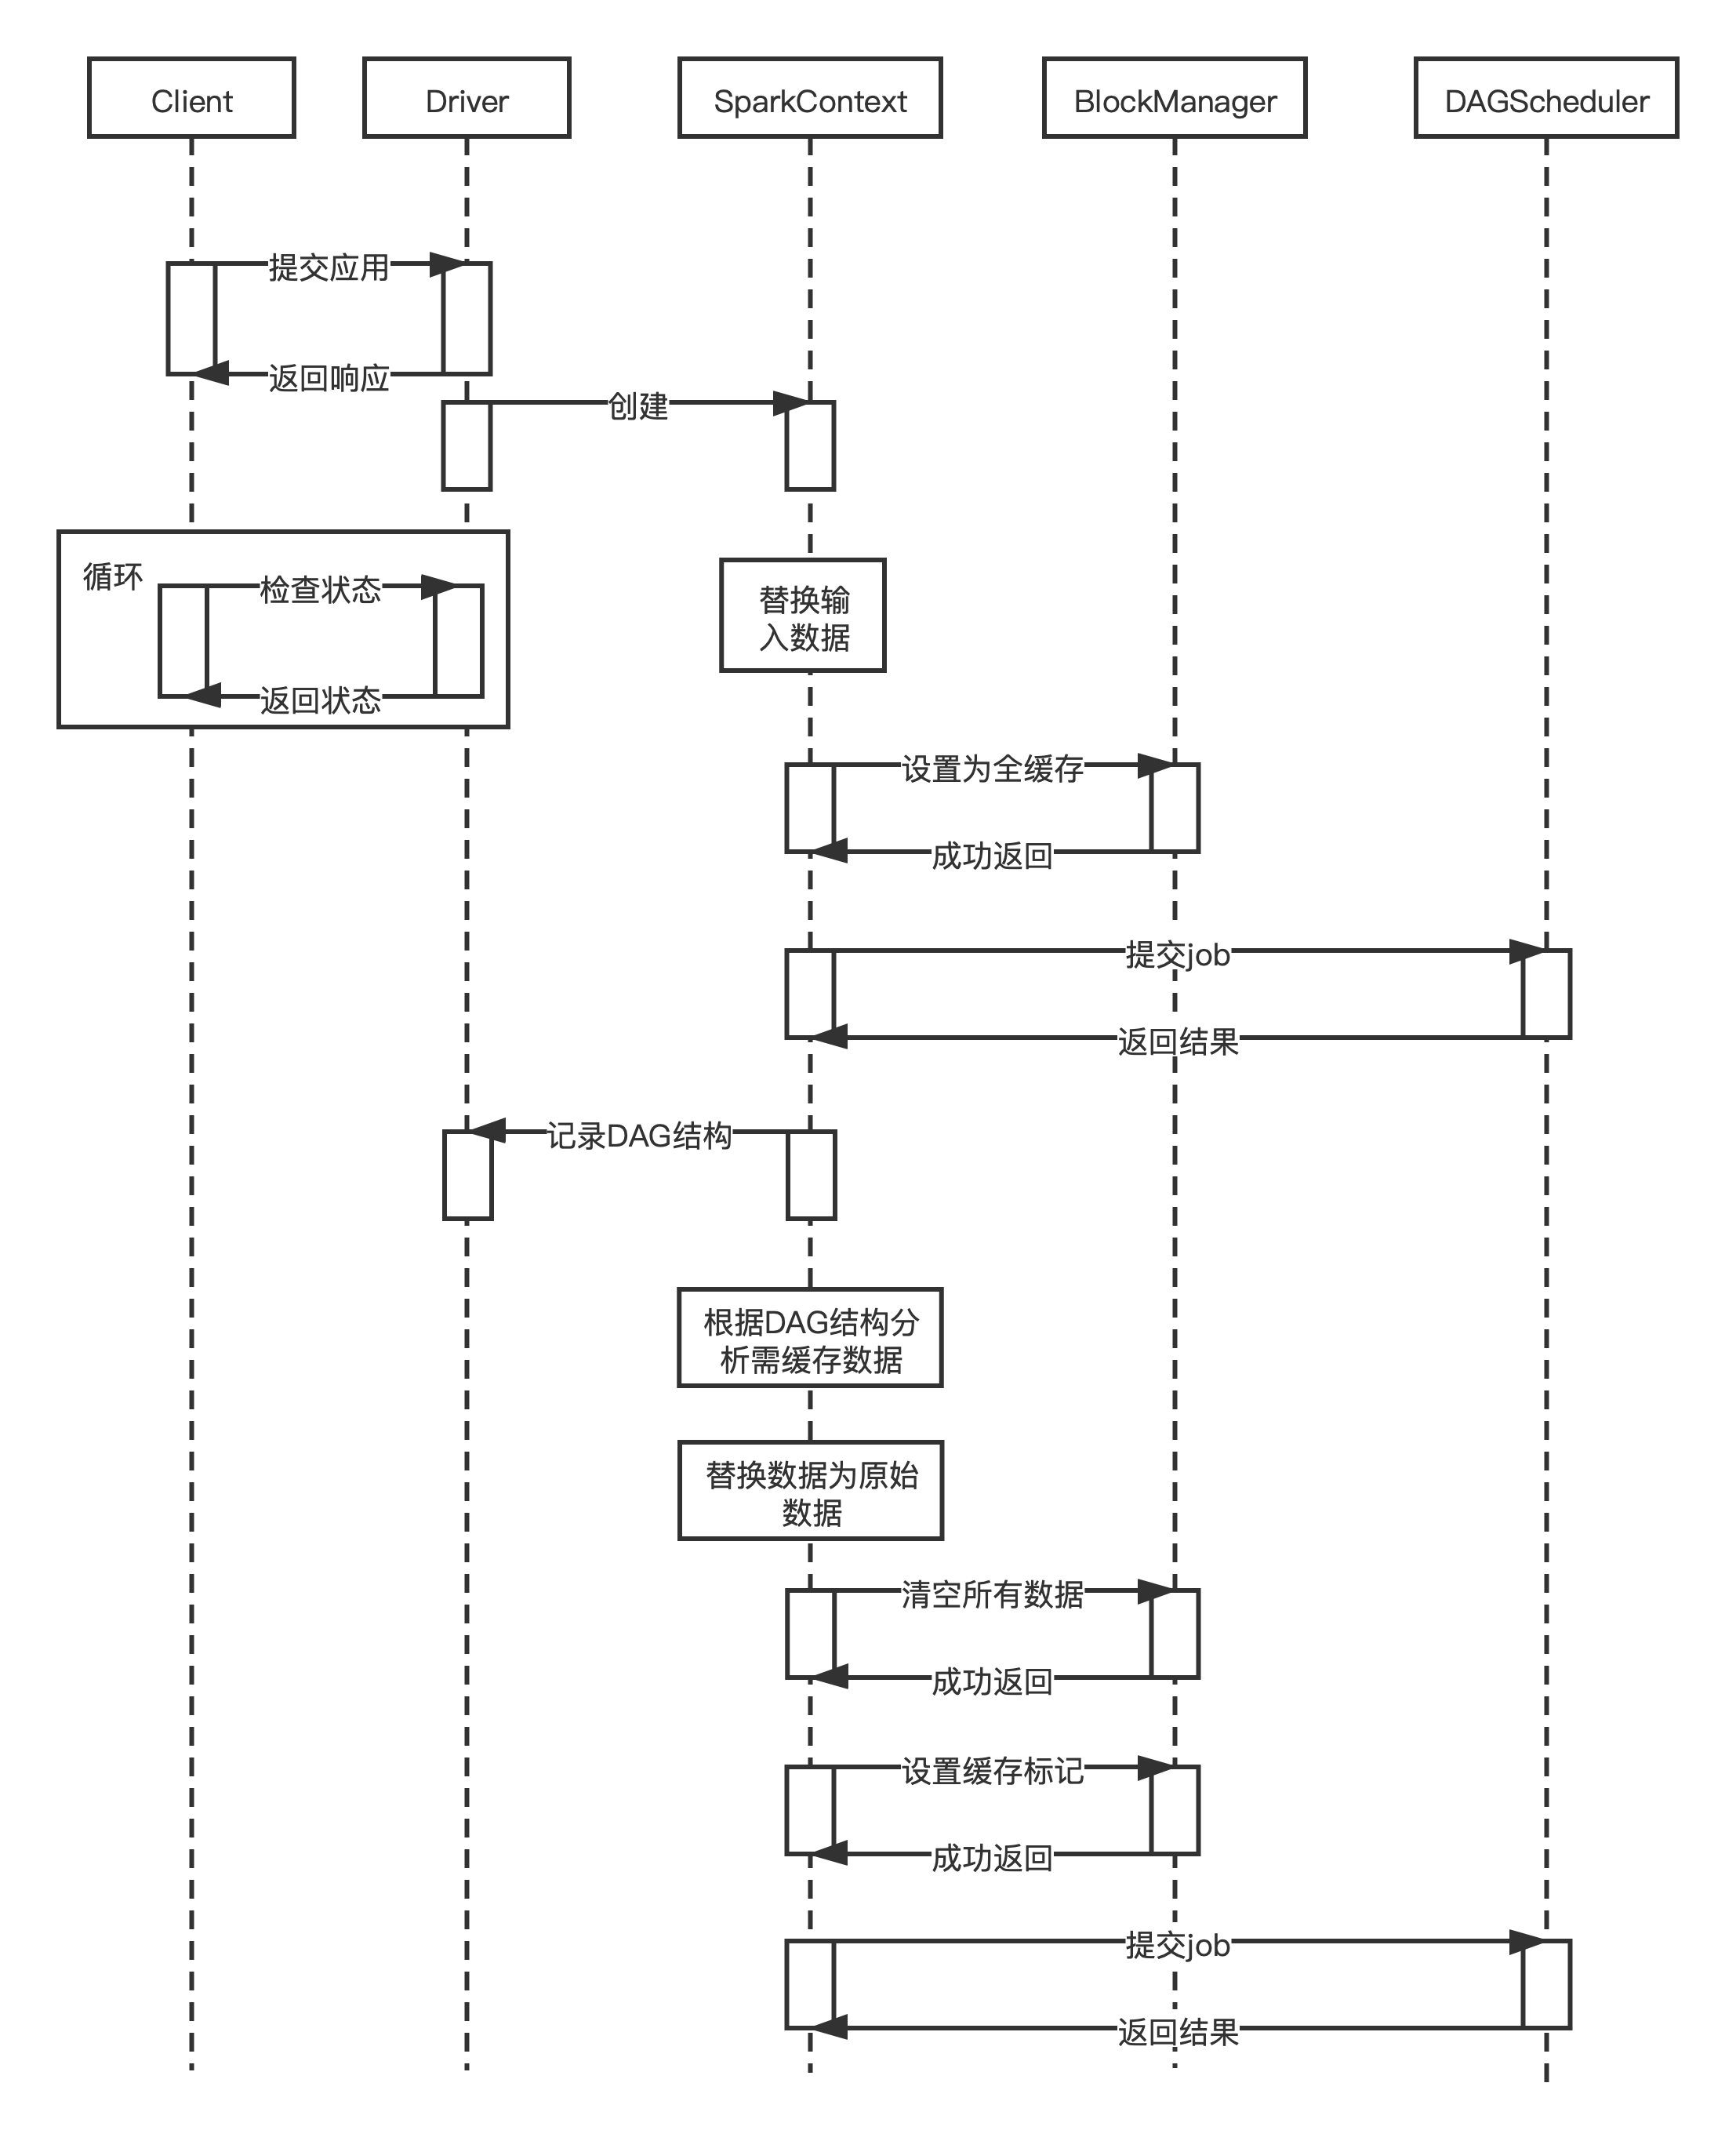
\includegraphics[width=1\textwidth]{Img/自动缓存流程图.png}
    \caption{自动缓存流程图}
    \label{fig:auto-cache}
\end{figure}

\begin{algorithm}  
    \caption{根据DAG图计算RDD使用频率}  
    \begin{algorithmic}[1] %每行显示行号  
        \Require DAG图根节点
        \Ensure 所有RDD使用频率
        \Function{CALCULATE\_FREQUENCY}{$RDD \ root, HashMap \ frequency$}  
            \State $id \gets root.getId()$
            \State $parent \gets root.getDependencies()$
            \For{$preRdd \in parent$}
                \State $preId \gets preRdd.getId()$
                \State $frequency[preId] \ frequency[preId] + 1$
                \State \Call{$CALCULATE\_FREQUENCY$}{$preRdd, \ frequency$}
            \EndFor
        \EndFunction  
    \end{algorithmic}
    \label{alg:cal-fre}
\end{algorithm}

\begin{algorithm}  
    \caption{清空缓存数据}  
    \begin{algorithmic}[1] %每行显示行号  
        \Require DAG图根节点
        \Function{CLEAN\_CACHE}{$RDD \ root$}  
            \State $root.unpersist()$
            \State $parent \gets root.getDependencies()$
            \For{$preRdd \in parent$}
                \State \Call{$CLEAN\_CACHE$}{$preRdd$}
            \EndFor
        \EndFunction
    \end{algorithmic}
    \label{alg:clean-cache}
\end{algorithm}


\begin{algorithm}  
    \caption{设置缓存标记}  
    \begin{algorithmic}[1] %每行显示行号  
        \Require DAG图根节点
        \Function{SET\_CACHE\_FLAG}{$RDD \ root, HashMap \ frequency$}
            \State $id \gets root.getId()$
            \State $rddFre \gets frequency[id]$
            \If{rddFre \ge 2}
                \State $root.STORAGE\_LEVEL \gets MEMORY\_ONLY$
            \EndIf
            \State $parent \gets root.getDependencies()$
            \For{$preRdd \in parent$}
                \State \Call{$SET\_CACHE\_FLAG$}{$preRdd, \ frequency$}
            \EndFor
        \EndFunction
    \end{algorithmic}
    \label{alg:set-cache}
\end{algorithm}

通过图\ref{fig:auto-cache}所示的流程,可以在第一次小规模计算结束之后得到整个DAG图的结构。然后通过算法\ref{alg:cal-fre}计算所有RDD节点的使用频率。得到频率之后便利整个DAG图,先调用unpersist接口清空小数据的缓存,再根据计算的到的频率设置各个RDD的STORAGE\_LEVEL之后修改输入节点的数据,替换为大规模数据,这样做有一下优点:

\begin{enumerate}
    \item 避免重复创建SparkContext对象,节约额外开销。在分析了自动缓存模块的实现原理之后可以发现因为需要通过运行整个应用获得DAG图,所以无法避免会带来一些额外开销。通过直接修改输入节点数据,就可以避免重复创建SparkContext对象,从而极大地减少了额外开销。
    \item 利用容错原理简化实现过程。通过流程图\ref{fig:auto-cache}可以设置rdd的缓存标记。设置完成之后只需要通过submitJob接口重新提交DAG图最后一个job即可。因为小规模数据缓存已经全部被清空,并且输入数据已经被替换,所以框架会根据基于血缘的容错原理从头开始执行整个DAG图。
\end{enumerate}

在第二次执行过程中,DAGScheduler会将job分为多个stage执行,在一个stage执行结束之后,会优化下一个stage的执行计划,此时根据调整自动缓存模块同步修改DAG图结构。实际上,目前自动执行框架只会做比较细粒度的执行计划,对DAG图整体结构并不会做出太大爱的调整。

\section{测试与性能分析}

为了测试自动缓存模块的效果,本文修改了Spark3.0的代码,实现了上述自动缓存模块的功能。然后通过SparkBench测试,下文也是使用SparkBench测试,本章简单的介绍以下SparkBench的功能和使用。

\subsection{SparkBench介绍}

SparkBench是Spark系统的基准性能测试项目,由IBM Watson研究中心的五名研究者发起,最后贡献给开源社区。SparkBench的测试项目覆盖了Spark最常见的四种应用:SQL查询、机器学习、图计算和流式计算。每种应用类型都选取了最常见的几个算法进行测试。SparkBench框架的测试结果包含系统资源消耗,计算时间,网络磁盘IO。所以可以比较全面地分析Spark系统的特点。官网也提供了论文。SparkBench支持表\ref{tab:workload}所示的负载。

\begin{table}
 \centering
 \caption{SparkBenck支持的负载}
 \label{tab:workload}
 \begin{tabular}{lcccl}
  \toprule
  应用类型 & 测试负载 \\
  \midrule
  机器学习 & 逻辑回归、支持向量机,矩阵分解  \\
  图计算 &  PageRank,SVD++,三角计数(Triangle Count) \\
  SQL查询 & Hive,RDDRelation  \\
  流式计算 & Twitter Tag , Page View  \\
  其他 &  Kmeans,线性回归,决策树,最短路径,标签传播,连通图,强连通图 \\
  \bottomrule
 \end{tabular}
\end{table}

SparkBench测试数据大部分都可以通过自带的数据生成器生成。SparkBench的使用也比较简单,分为以下三步:

\begin{enumerate}
    \item 修改<workload>/conf/env.sh文件,配置测试配置数据
    \item 使用<workload>/bin/gen\_data.shs生成测试数据,这个脚本会根据配置的数据生成指定大小的测试数据
    \item 调用<workload>/bin/run.sh运行测试负载
\end{enumerate}

测试样例运行完毕之后,测试数据会存放在num目录下面。包含作业运行过程中的资源使用情况,作业执行时间。资源使用情况包含CPU、内存的使用情况,磁盘和网络IO的使用情况。

\section{测试与分析}

本实验在一台PC电脑上实现,通过参数设置Spark为local mode,同时设置Spark为local模式运行。给Spark框架分配了8GB的内存。6个CPU。具体硬件配置与原件版本如表\ref{tab:setup}所示。

\begin{table}
 \centering
 \caption{测试环境硬件配置与软件版本}
 \label{tab:setup}
 \begin{tabular}{lcl}
  \toprule
  配置项 & 配置信息 \\
  \midrule
  CPU &  2.6GHz 6-core 9th\-generation Intel Core i7 processor \\
  内存 & 16GB of 2666MHz DDR4 memory  \\
  磁盘 &  512GB of SSD storage \\
  Spark版本 & 3.0.0  \\
  Hadoop版本 &  3.2 \\
  Scala版本 & 2.11.8  \\
  JDK版本 &  java\-1.8.0\_231 \\
  操作系统 & macOS 11 Big Sur  \\
  开发环境 &  IntelliJ IDEA 11.1.4 \\
  \bottomrule
 \end{tabular}
\end{table}

本文选用了逻辑回归、HIVE、PageRank、矩阵分解四个测试负载,在不同输入数据大小情况下,测试对比了自动缓存模块的效果。首先我对四个测试样例进行了测试,统计了Shuffle数据、Stage数量、Task数量等信息。通过测试可以发现不同的测试负载各有特点。比如对于逻辑回归类型应用,它并不存在shuffle操作,所以shuffle的读写数据都为0。对于HIVE应用,因为HIVE SQL查询最终生成的逻辑执行计划是一样的,又因为stage是根据宽依赖也就是shuffle依赖确定的,所以stage数量是相同的,但是因为数据量变大之后分区数量也随之变大,每一个分区对应一个task,所以随着数据量变大,task数量也会变多。对于PageRank算法,每次迭代后如果和上次的排名没有区别算法就认为已经收敛,然后推出结束了,数据规模比较小时收敛速度比较快,数据量大的情况下收敛速度变慢,迭代的轮数也会变多,导致stage数量也会变多。

\begin{table}
 \centering
 \caption{SparkBenck支持的负载}
 \label{tab:workload}
 \begin{tabular}{lccccccccccccccccl}
  \toprule
  负载名称 & 输入数据大小 & Shuffle 读/写 数据量 & Stage 数量 & Task 数量 \\
  \midrule
  逻辑回归 & 2G & 0G/0G & 3 & 431 \\  
  逻辑回归 & 4G & 0G/0G & 4 & 513 \\  
  逻辑回归 & 8G & 0G/0G & 5 & 1152 \\  
  逻辑回归 & 16G & 0G/0G & 7 & 2254 \\  
  HIVE & 2G & 2.7G/2.8G & 12 & 2927 \\  
  HIVE & 4G & 4.6G/4.8G & 12 & 6272 \\  
  HIVE & 8G & 10.3G/11.6G & 12 & 10048 \\  
  HIVE & 16G & 21.3G/22.7G & 12 & 20174 \\ 
  PageRank & 2G & 7.4G/9.4G & 6 & 1578 \\  
  PageRank & 4G & 15.4G/18.6G & 8 & 3481 \\  
  PageRank & 8G & 27.7G/31.8G & 13 & 5727 \\  
  PageRank & 16G & 62.3G/67.7G & 21 & 12247 \\
  矩阵分解 & 2G & 0.7G/0.9G & 9 & 394 \\  
  矩阵分解 & 4G & 1.2G/1.3G & 20 & 757 \\  
  矩阵分解 & 8G & 2.8G/3.1G & 43 & 1556 \\  
  矩阵分解 & 16G & 5.0G/5.4G & 81 & 4302\\  
  \bottomrule
 \end{tabular}
\end{table}

之后本文测试了自动缓存模块的效果,测试方法是修改了SparkBench测试负载的代码(在legacy分支),将代码中的cache调用全都删除,修改后运行添加了自动缓存模块的Spark框架。之后再与未修改的原生Spark框架进行对比。测试结果如图\ref{fig:auto-cache}所示。对于四个测试样例,一共进行了4组测试。每组测试分为两个样例,分别是手动缓存测试程序和自动缓存模块的对比。可见,自动缓存因为需要执行一遍得到整个DAG图结构,所以不可避免会导致一些额外的开销。使用自动缓存的模块实际运行时间变化不大。总体来说,因为使用自动缓存模块对于迭代式运算作业会带来12\%的额外开销,对于SQL类作业会带来3\%的额外开销。
\begin{figure}
    \centering
    \begin{subfigure}[b]{0.45\linewidth}
      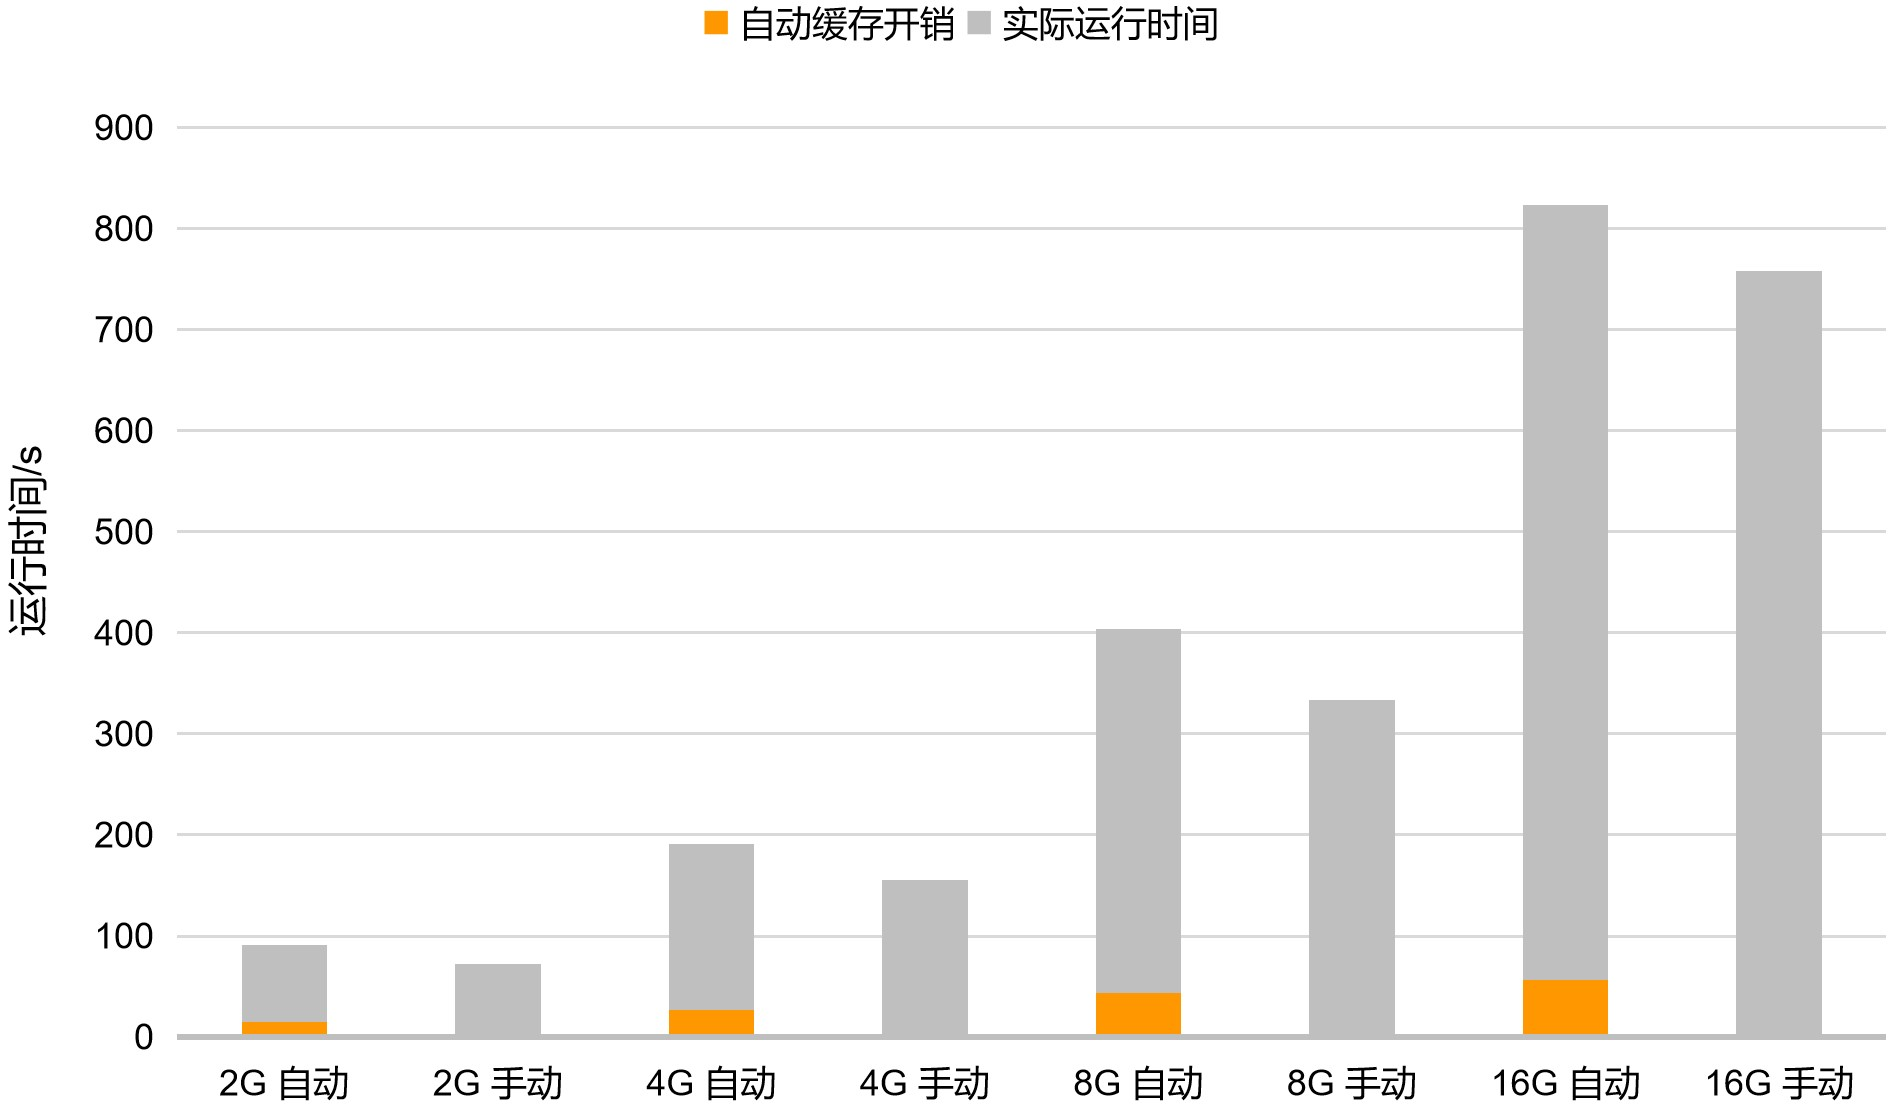
\includegraphics[width=\textwidth]{Img/lr1.jpg}
      \caption{逻辑回归测试}
      \label{fig:lr-auto-cache}
    \end{subfigure}%
    ~% add desired spacing
    \begin{subfigure}[b]{0.45\linewidth}
      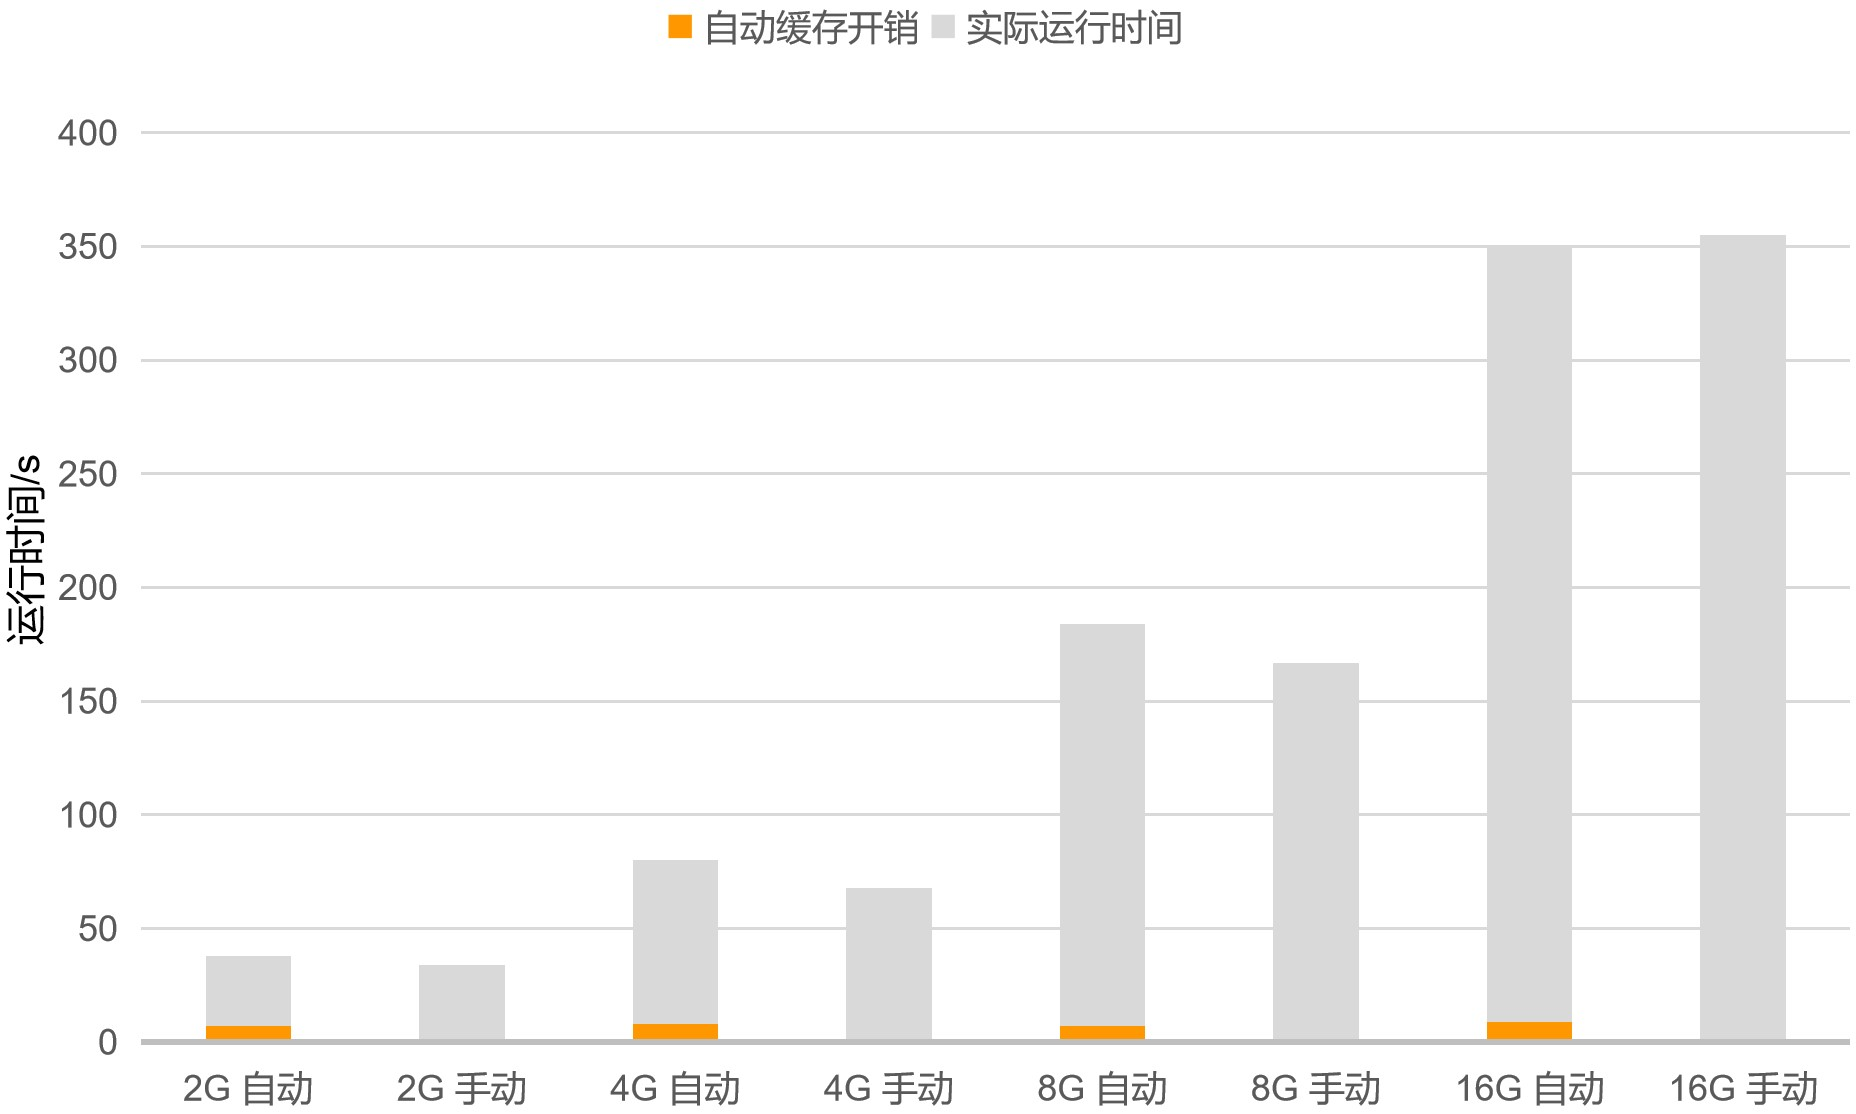
\includegraphics[width=\textwidth]{Img/hive1.jpg}
      \caption{HIVE SQL测试}
      \label{fig:hive-auto-cache}
    \end{subfigure}
    \\% line break
    \begin{subfigure}[b]{0.45\linewidth}
      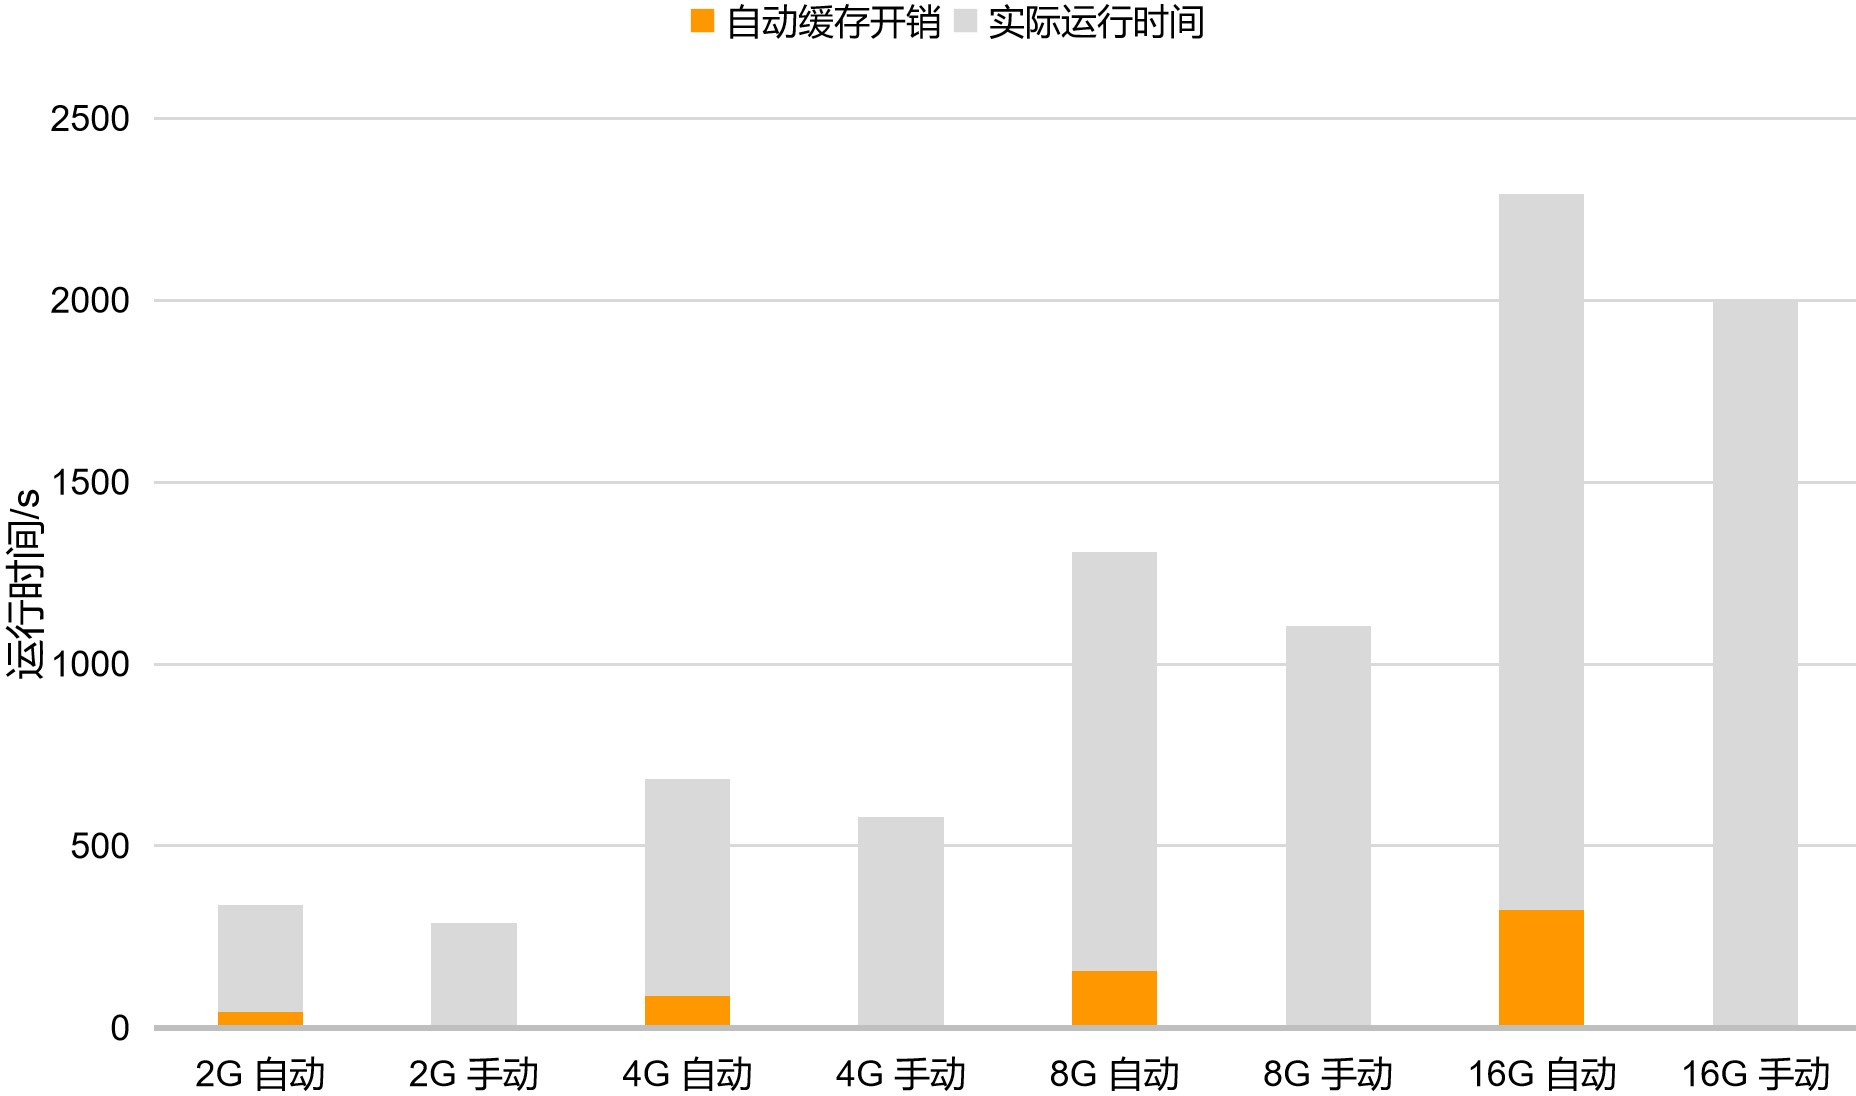
\includegraphics[width=\textwidth]{Img/pg1.jpg}
      \caption{PageRank测试}
      \label{fig:pagerank-auto-cache}
    \end{subfigure}%
    ~% add desired spacing
    \begin{subfigure}[b]{0.45\linewidth}
      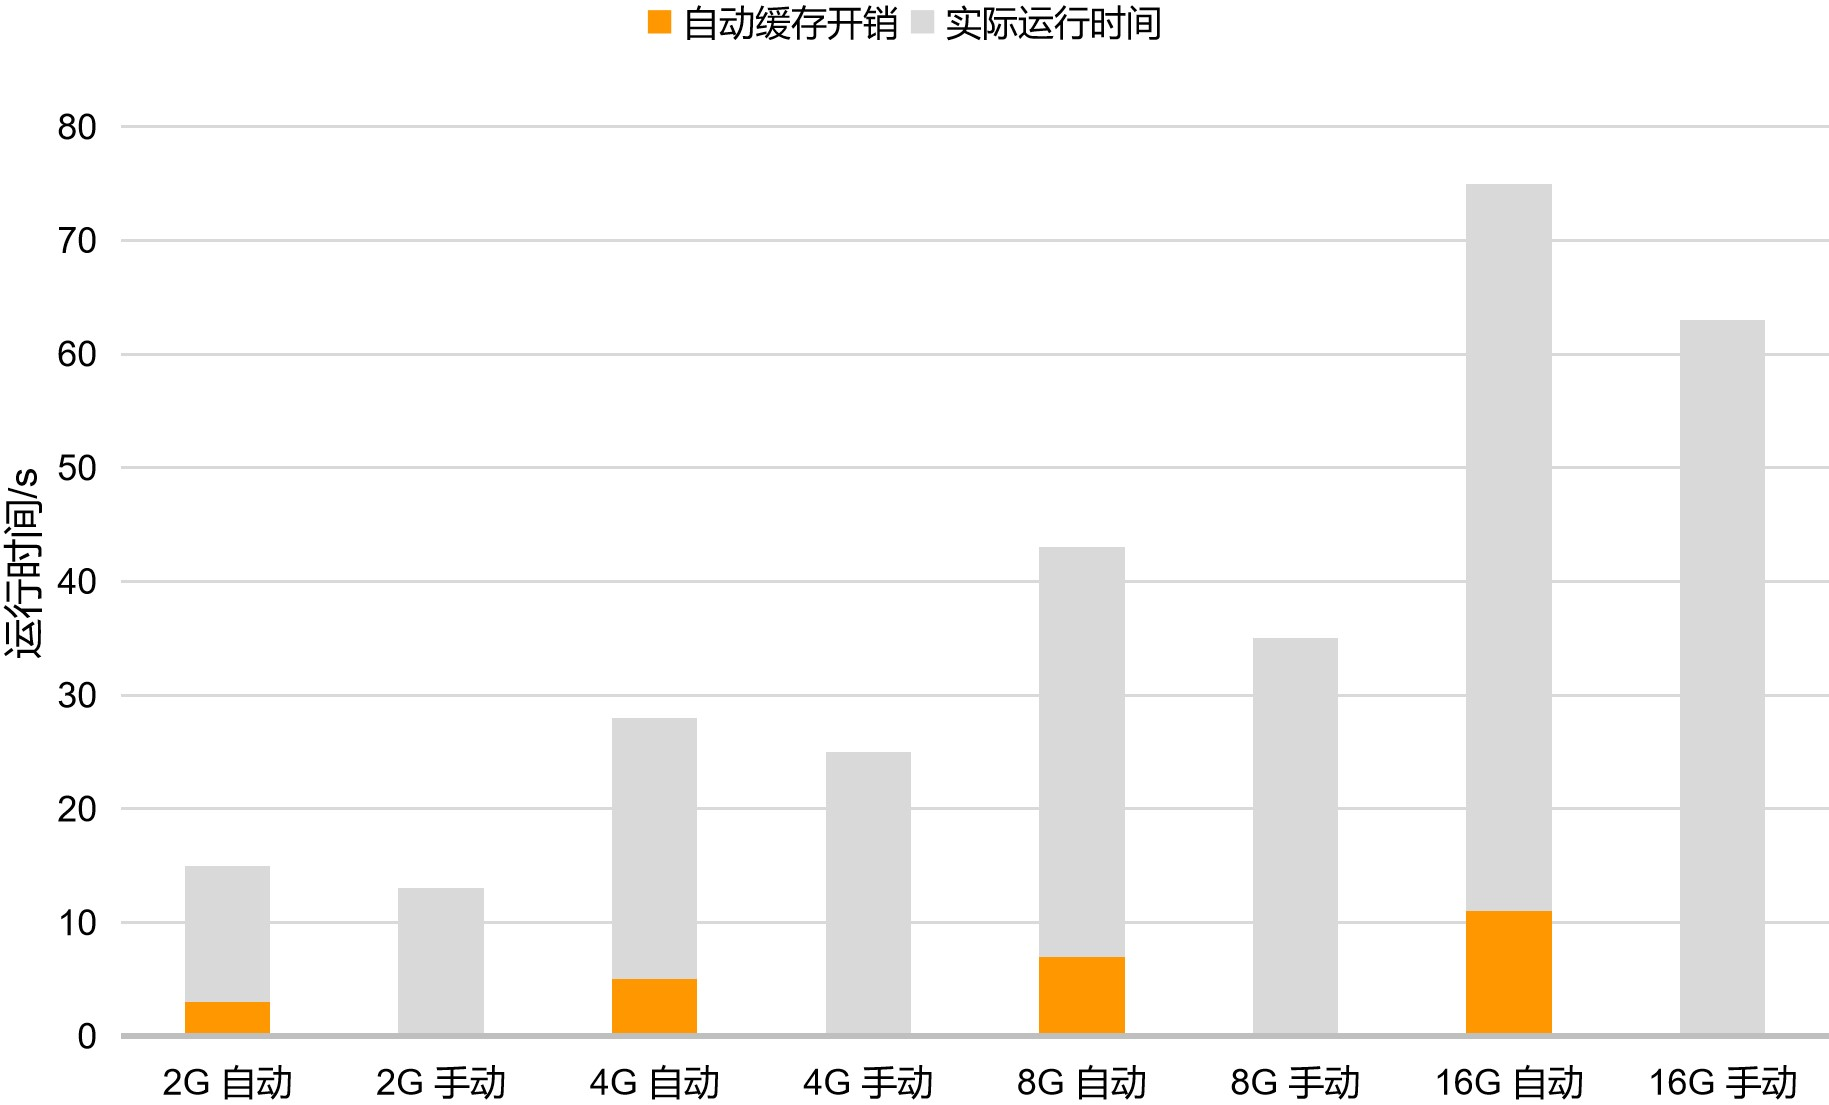
\includegraphics[width=\textwidth]{Img/mx1.jpg}
      \caption{矩阵分解测试}
      \label{fig:matrix-auto-cache}
    \end{subfigure}
    \caption{自动缓存测试}
    \label{fig:auto-cache}
\end{figure}

从图\ref{fig:autocache-2}可以看到,对于逻辑回归、PageRank和矩阵分解来说,额外开销会随着数据规模变大而变大,这与自动缓存和算法实现原理有关。因为这三种算法随着数据规模变大,迭代次数也会变多,所以第一次执行也需要迭代很多次才能得到DAG图结构,就会造成比较大的延迟。而对于HIVE SQL作业来说,随着数据规模变大额外开销并不会随之变化太多。这是因为对于SQL查询作业来说,在SQL转化得到的逻辑执行计划并不会随着输入数据变化,所以不同数据规模的自动缓存模块执行的逻辑执行计划都是一样的,就不会有太大的差别。

\begin{figure}
    \centering
    \begin{subfigure}[b]{0.45\linewidth}
      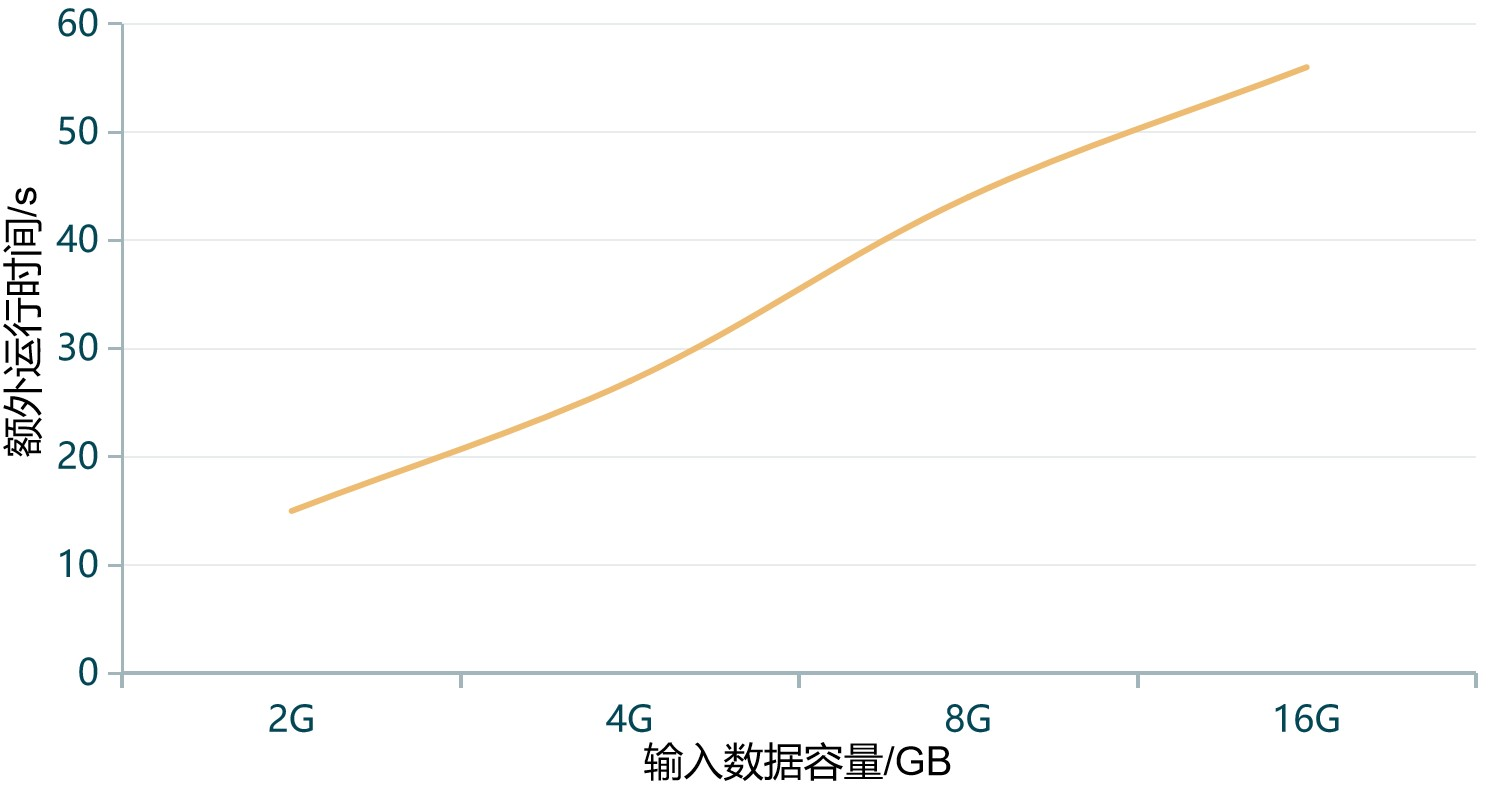
\includegraphics[width=\textwidth]{Img/lr2.jpg}
      \caption{逻辑回归测试}
      \label{fig:lr-ac-2}
    \end{subfigure}%
    ~% add desired spacing
    \begin{subfigure}[b]{0.45\linewidth}
      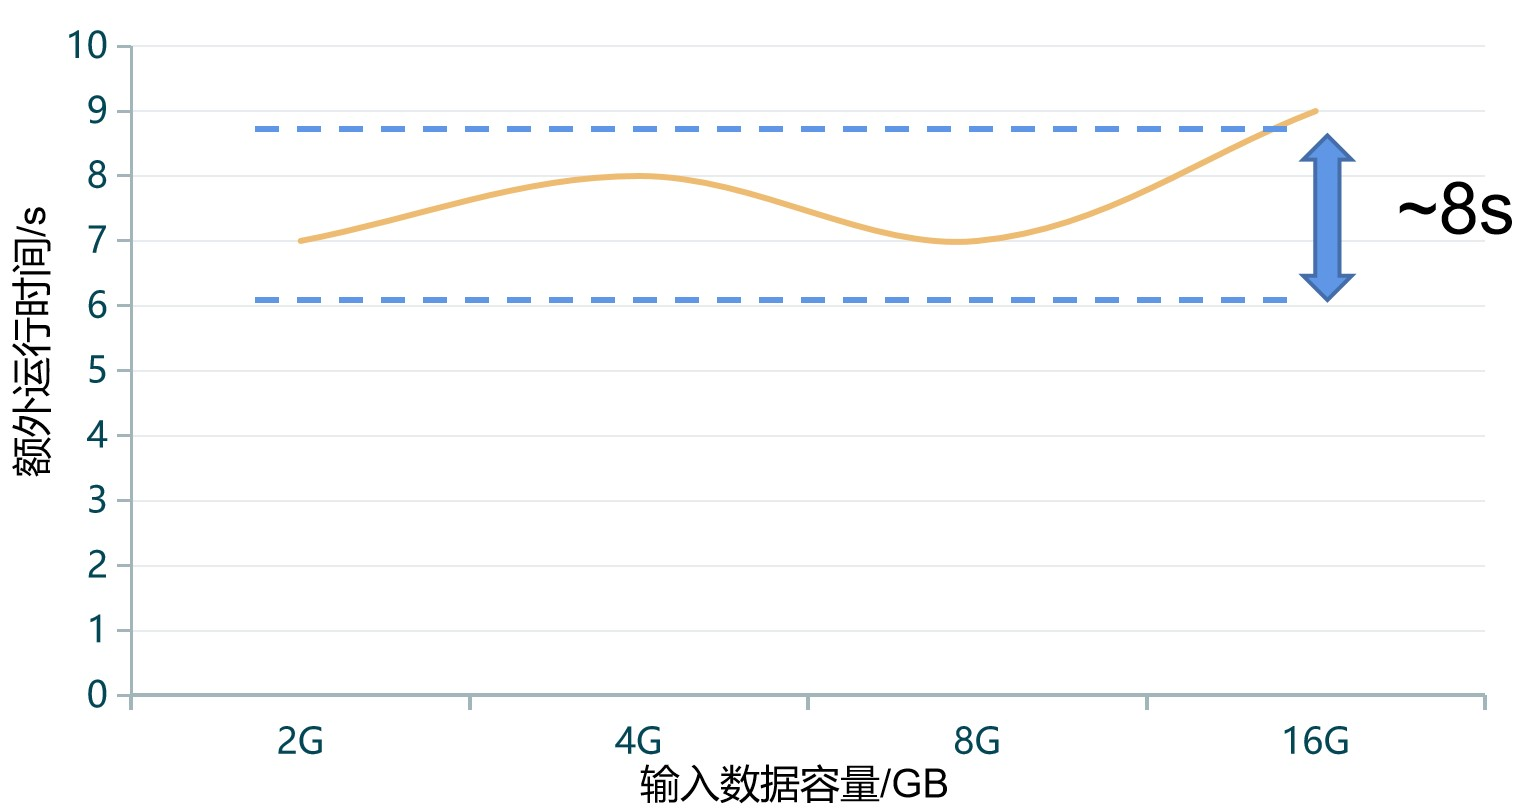
\includegraphics[width=\textwidth]{Img/hive2.jpg}
      \caption{HIVE SQL测试}
      \label{fig:hive-ac-2}
    \end{subfigure}
    \\% line break
    \begin{subfigure}[b]{0.45\linewidth}
      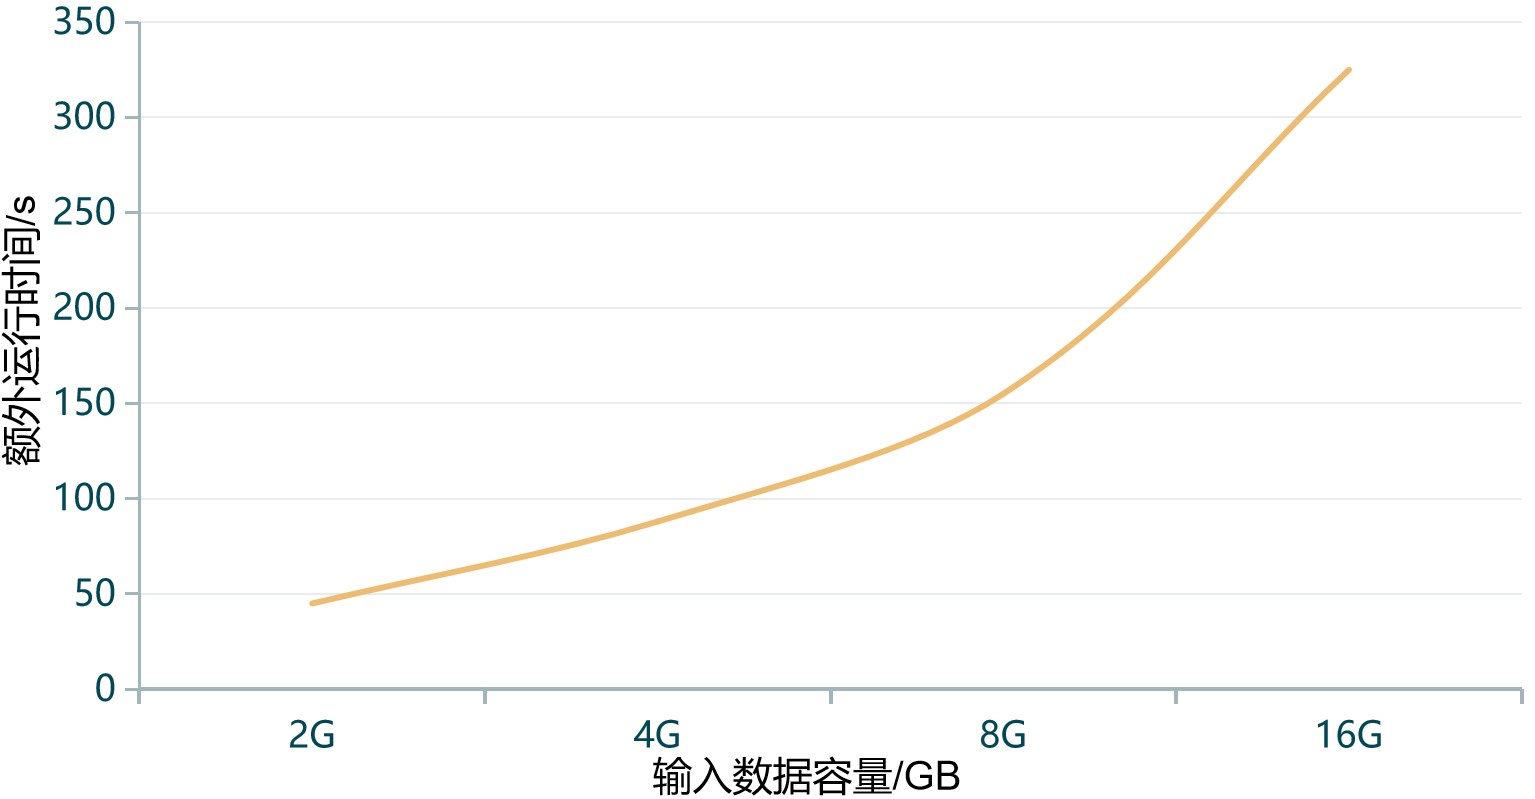
\includegraphics[width=\textwidth]{Img/pg2.jpg}
      \caption{PageRank测试}
      \label{fig:pagerank-ac-2}
    \end{subfigure}%
    ~% add desired spacing
    \begin{subfigure}[b]{0.45\linewidth}
      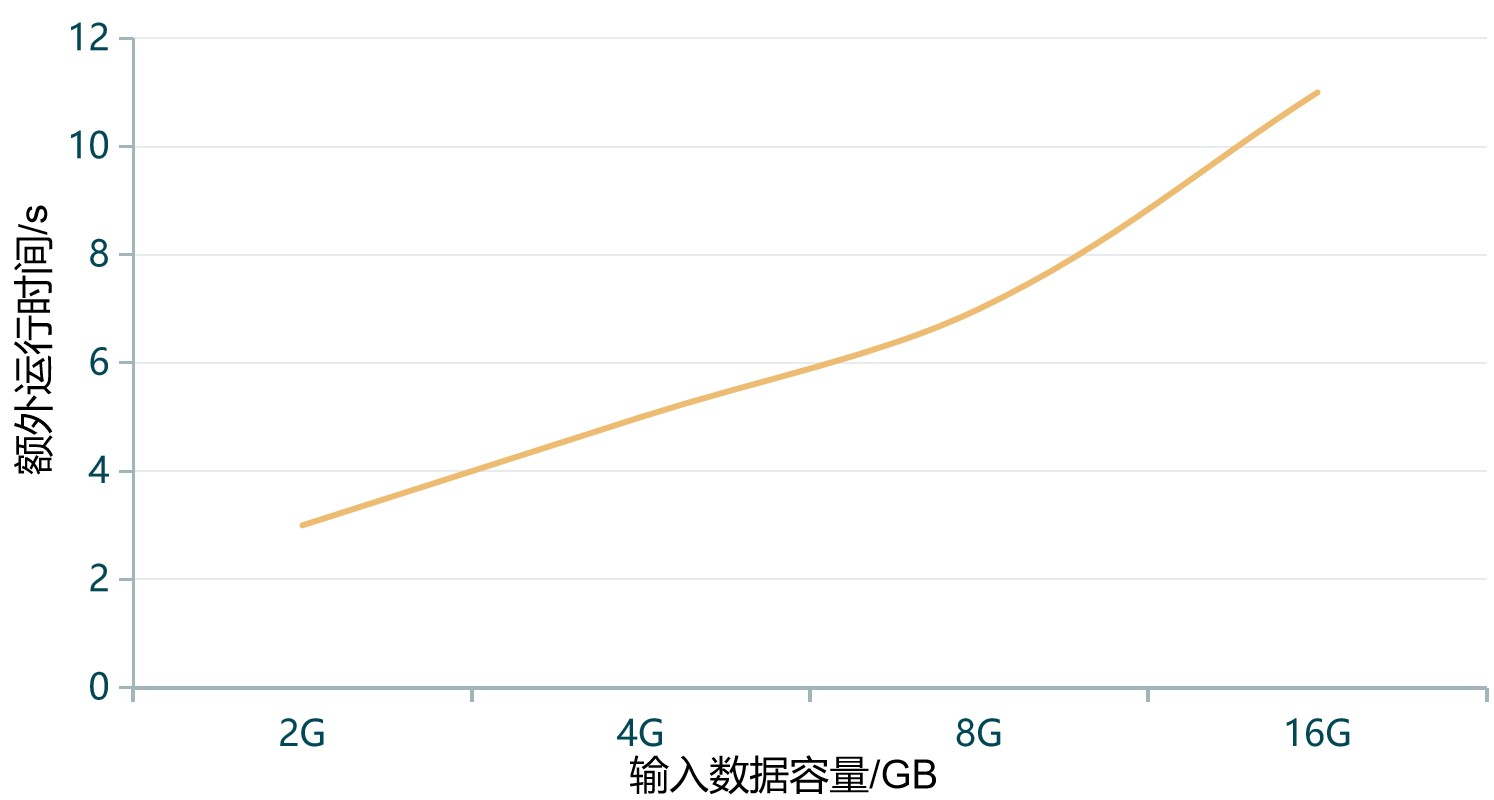
\includegraphics[width=\textwidth]{Img/mx2.jpg}
      \caption{矩阵分解测试}
      \label{fig:matrix-ac-2}
    \end{subfigure}
    \caption{自动缓存额外开销测试}
    \label{fig:autocache-2}
\end{figure}

总结可以总结以下结论,自动缓存模块对于SQL作业效果比较好,随着数据规模变大,额外开销占比越来越小。而对与PageRank这类迭代式计算应用则效果一般,因为这类应用随着数据规模变大,迭代次数也会变大,额外开销也会随着迭代次数变多而随之变大。

\section{本章总结}

本章介绍了Spark模块底层的原理以及最新的Spark自适应执行特性。之后设计并实现了自动缓存模块,自动缓存模块通过分析DAG图结构得到需要缓存的数据并自动将其缓存到内存之中。最后对自动缓存模块进行了一系列的测试,实验测试结果表明自动缓存模块适合SQL查询类作业,因为这类作业不同数据规模的执行计划相同,所以数据规模越大自动缓存模块额外开销占应用运行总时间越短。但是不太适合迭代计算式作业,因为大规模数据迭代次数变多额外开销也会随之变大。最后经过计算,对于迭代式计算和SQL作业,自动缓存模块平均额外计算开销占作业总执行时间的12\%和3\%。


\chapter{一种基于DAG作业运行时信息及拓扑结构的缓存替换策略的设计与实现}\label{chap:guide}

\section{Spark系统缓存替换策略分析}
\subsection{Spark系统的中的LRU策略}
\subsection{LRU缓存替换策略存在的缺陷}
\section{基于DAG作业运行时信息及拓扑结构的缓存替换策略的设计}
\section{基于DAG作业运行时信息及拓扑结构的缓存替换策略的实现}
\section{基于DAG作业运行时信息及拓扑结构的缓存替换策略测试与性能分析}
\section{本章总结}
\chapter{容错性加强的自动缓存清理模块}\label{chap:clean}

\section{内存管理模块分析}

Spark框架由Scala语言编写。Scala语言是一种运行在JVM(Java Virtual Machine)的函数式编程语言。函数式编程语言相比于C++、Java等命令式编程语言的优点是将数据进行了分类,分为可变数据数据variable和不可变数据value。同时也提供了非常适合并行编程的函数式编程接口。函数式语言的这种特点就让它天然适用于分布式并行大数据处理领域。Scala语言还有一个独特的优势就是它是运行在JVM之上的,这就让Scala语言可以运行在所有支持JVM的平台上,这就使得Scala具有非常好的跨平台特性。但是对于Spark框架来说,他有完全独立的内存管理模块BlockManager。BlockManager也是运行在JVM上的一个进程。

\begin{figure}[htbp]
    \centering
    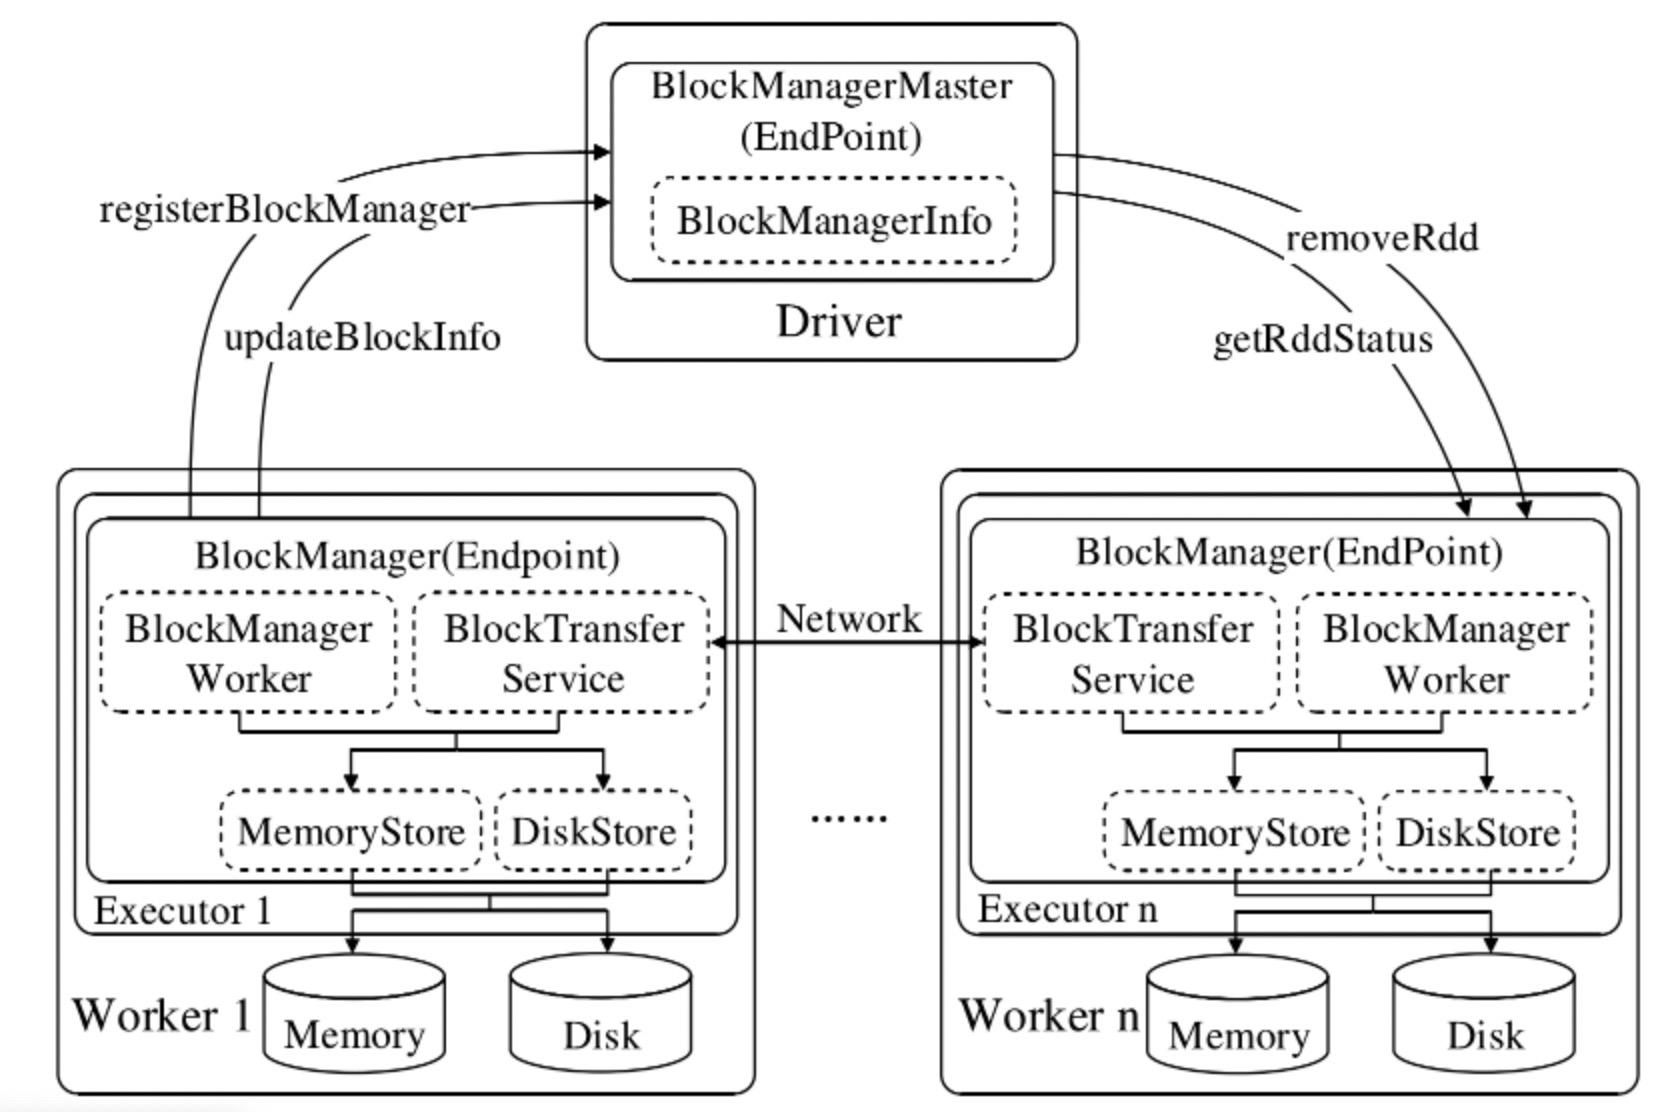
\includegraphics[width=0.99\textwidth]{Img/block-manager.jpg}
    \caption{BlockManager结构图}
    \label{fig:block-manager}
\end{figure}

\subsection{内存管理模块潜在问题}

BlockManager和JVM都有管理内存的功能,但是两者完全隔离,这就会有潜在的问题。BlockManager内存管理的原理非常简单。用户提交Spark应用的时候会通过配置文件指定Executor使用的内存总量,之后框架会向JVM申请内存创建Executor以及内部的BlockManager。BlockManager初始化之后会开始管理Executor整个内存空间。BlockManager向外提供了非常简单的接口,Get接口和Put接口。Get接口的参数为RDD数据的ID,如果数据存储在磁盘或者内存之中BlockManager就会返回具体的地址。Put接口的参数是RDD的应用和存储级别,比如MEMORY\_ONLY、DISK\_ONLY等,BlcokManager会根据存储级别将数据存储在不同位置。

框架的内存模型如图\ref{fig:memory-model}所示。Spark框架内存模型分为以下几个部分:Storage区域,Execution区域,Other区域。Other区域主要用于用户程序定义的数据结构。Execution内存用于框架执行,比如计算RDD的分区时数据就全部存储在Execution区域。Execution区域的内存有一个特点就是会主动地回收内存。他使用的方法是类似与引用计数的算法。比如一个图\ref{fig:simpl-dag}所示的简单的三个节点的计算图。计算得到数据B的时候B的数据就存储在Execution区域。因为计算C还会使用数据B所以数据B并不会立刻被替换出去。但是A会被立刻删除。在以后计算E的时候又会使用到数据A,但是数据A早已被删除,这就会造成数据丢弃,框架会通过容错算法重新计算数据A。

\begin{figure}[htbp]
    \centering
    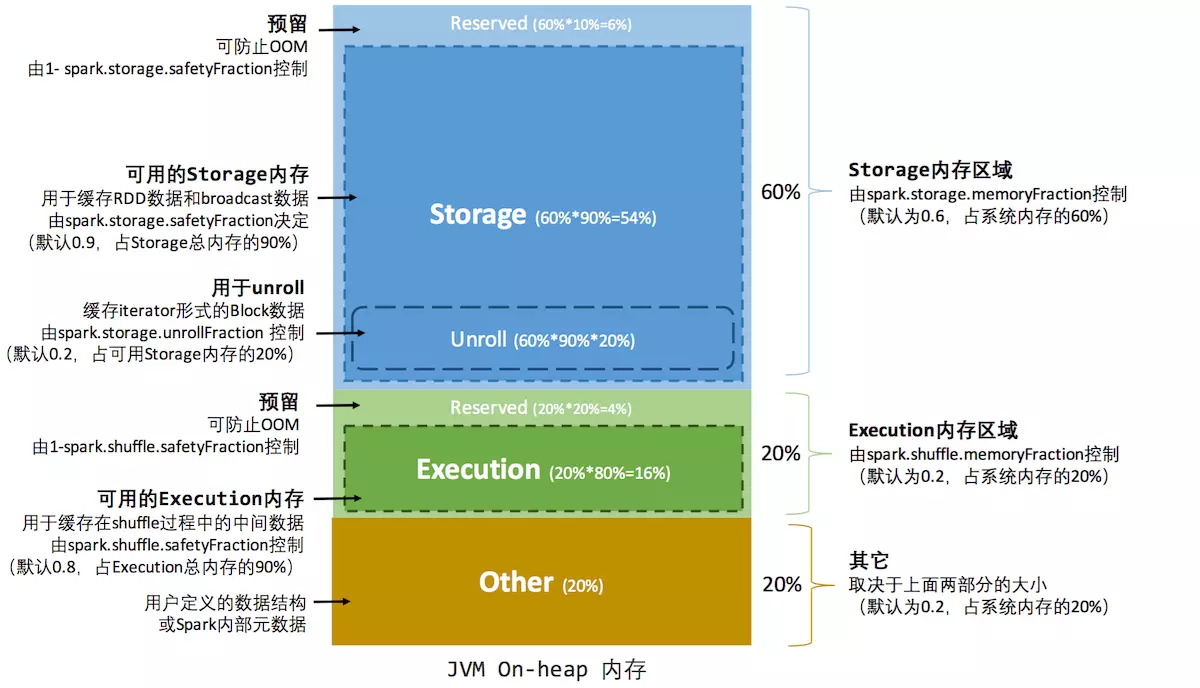
\includegraphics[width=0.99\textwidth]{Img/memory-model.png}
    \caption{内存模型}
    \label{fig:memory-model}
\end{figure}

对于内存管理来说是BlockManager内部的MemoryStore负责的。MemoryStore内部简单地通过一个整数变量记录Executor节点空闲的内存,当收到缓存请求时,MemoryStore会比较空闲空间和需要缓存的数据大小,如果空闲空间大于缓存数据就会保存缓存数据的引用在LinkedHashMap中,这样就能够避免数据被清理。数据放入LinkedHashMap后memoryStore模块会在数值上减少剩余缓存的总量。

通过详细分析Spark框架缓存管理模块的原理可以发现存在着潜在的问题。因为Spark框架的内存管理和JVM虚拟机的内存管理是完全独立的。Spark框架申请内存的行为是一次性的,但是Spark框架释放内存行为和JVM是不同步的。Spark内存管理依赖于JVM的内存回收机制。JVM的自动给回收机制是通过可达性分析实现的。通过从垃圾回收根节点对象出发向下搜索,搜索到的节点为引用链,如果有一些对象没有任何引用链相连,那么这个对象对于内存回收根对象是不可达的,所以将其判定为可回收对象。JVM实际的内存回收原理要复杂得多。根据对内存分析过程的分析可以看到JVM内存回收过程需要进行大量的计算判断,并不能实时地回收内存对象。然而Spark框架的unpersist调用会释放MemoryStore中的RDD对象引用,所以从Spark框架视角看来内存回收立刻就完成了,这就会造成了潜在的风险。对于以下这种场景就有可能超过内存使用上限,造成JVM内存使用超限错误(OOM,Out of Memory error)。具体场景是这样的,Spark应用在执行过程中通过cache调用在内存中缓存了很多RDD数据。缓存空间所剩无几,此时有新的缓存需求,Spark框架就会通过缓存替换策略替换一定数量的数据腾出缓存空间。然而此时JVM内存并没有立刻被回收,但是MemoryStore模块已经认为有了足够的空闲缓存空间,就将新的数据写入缓存空间之中,这就造成了Spark框架使用的内存总量超过了实际向JVM虚拟机申请的总内存,JVM就会杀死Spark框架相关的进程,这就会导致Spark框架奔溃。如图\ref{fig:oom}所示,在第二次内存时因为实际内存并没有释放,就会导致OOM问题。

\begin{figure}[htbp]
    \centering
    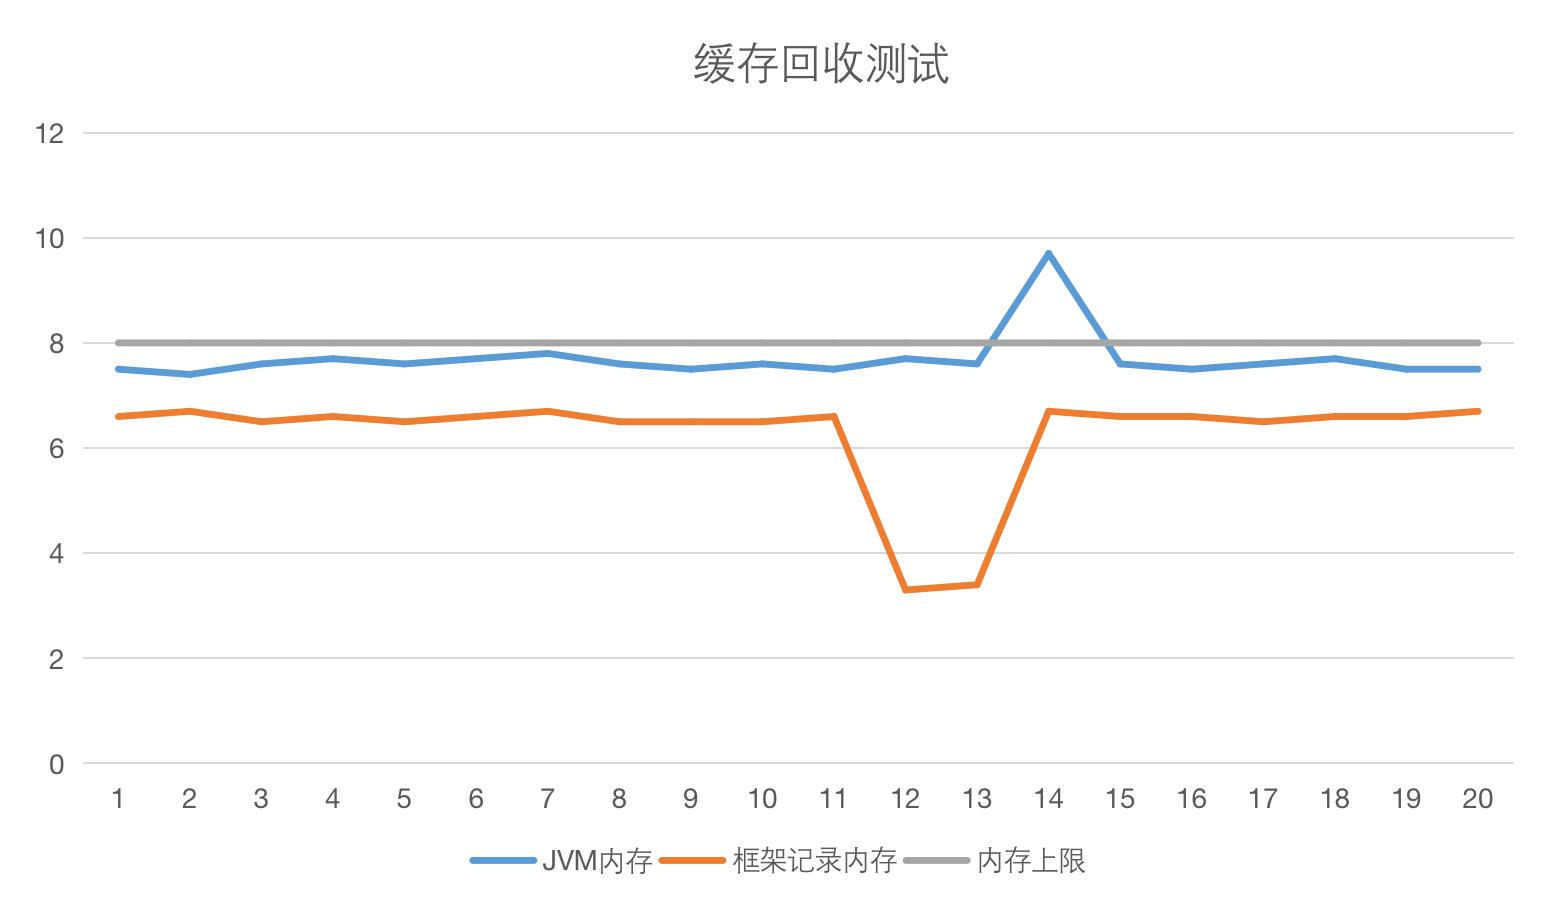
\includegraphics[width=0.99\textwidth]{Img/oom.png}
    \caption{oom问题分析图}
    \label{fig:oom}
\end{figure}


通过分析可以看到Spark框架目前的缓存管理机制是存在着一些潜在的风险的。事实上Spark官方也认识到了这个问题,官方提供的解决方案是设置一个冗余缓冲区,这样就能在一定程度上避免OOM的问题。但是这种解决方案也有一些问题,就是会造成大量内存资源的浪费。

\section{容错性加强的缓存清理模块设计与实现}

\subsection{缓存清理模块设计}

根据对上一节对Spark框架缓存机制的深入分析可以看到目前存在的潜在的问题。官方的解决方法一方面无法完全解决问题,另一方面还会浪费很多内存空间。所以本文从一个新的角度出发来解决这个问题。通过主动清理缓存中的缓存数据,就可以减少减少缓存空间的负载,避免因为负载过高导致内存使用超限的问题。

具体的设计要根据Spark框架的原理来实现,Spark应用提交给Spark框架之后会被解析成一个DAG图执行。通过对DAG图的分析就可以得知什么时候应该清理数据。DAG图中每个点都是RDD数据,DAG图中的边是RDD数据的转换操作。所以对于DAG图中的一个点,它有多少个出边就说明它会在接下来的计算中会被使用多少次。通过对DAG图的分析,就可以得到每个RDD数据在今后计算过程的使用次数n,实际上就是计算节点的出边个数。在计算的过程中,执行一个边的转化操作就将RDD的使用次数减一。这样当RDD的使用次数减为0的时候就说明在正常情况下不会再使用这个RDD数据。此时就可以主动清理MemoryStore模块中的缓存数据。

还有一个问题需要考虑就是作业的容错性。在正常不出错的情况下,在发现RDD数据不会再被使用时就可以清理缓存数据,这种方式可以让缓存空间中的冗余数据最少。然而这种非常激进的缓存清理方式也有它的问题。在出错场景下,Spark框架会根据DAG图的拓扑关系向上游寻找缓存数据,如果找到了缓存数据就可以迅速重新计算丢失的数据,但是如果清理了所有的冗余数据,Spark框架就会从DAG图的输入节点处读取输入数据重新开始计算,这样就会对Spark应用造成巨大的计算延迟。

为了兼顾容错性,可以在清理缓存数据时有选择地保留部分数据。将当前正在计算的RDD数据定义为0,DAG图中每条边的距离为1。具体策略是保存距离正在计算RDD数据小于等于2的数据。这种策略是出于以下考虑,要通过距离为1的RDD数据计算当前RDD数据,所以距离为1的RDD数据肯定需要保存在缓存空间之中。对于距离为2的数据,在计算出错,数据丢失情况下,框架可以通过距离为2的缓存数据迅速重新恢复计算。在小概率场景下距离为2的数据也会丢失,这种小概率场景就只能通过重新计算完成。通过这种设计,通过保留少量冗余数据就可以兼顾系统的容错性。

\subsection{缓存清理模块实现}

这里举一个例子,如图\ref{fig:ft1}所示,黄色节点是正在计算的RDD数据,所有黄色节点的距离为0,黄色RDD节点需要使用距离为1的虚线框中的数据计算得到,所以1号虚框中的数据要保存在内存之中加速计算。在正常计算过程中是只需要使用1号虚框中的数据的,所以灰色节点都可以从缓存中清除出去,从而可以提高缓存空间利用率。然而这种方式的容错性却非常差,在出错场景下会造成严重的重复计算开销。例如图\ref{fig:ft1}所示,红色节点是出错节点,因为在分布式计算数据存在多个机器上,如果某个机器发生问题就会导致这个机器上的数据全部丢失,假设红色节点的数据全部丢失,根据Spark框架的容错原理就需要根据DAG拓扑关系重复计算,具体来说就会计算图\ref{fig:ft1}中红色框中的所有数据,这就会造成大量的重复计算开销。

\begin{figure}[htbp]
    \centering
    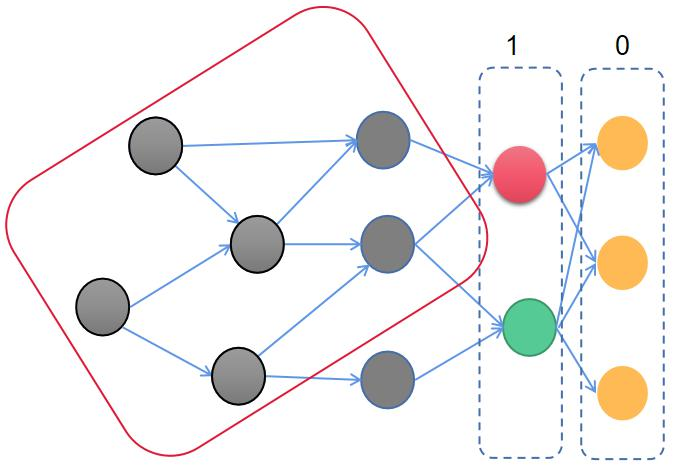
\includegraphics[width=0.6\textwidth]{Img/ft1.png}
    \caption{出错场景重复计算问题}
    \label{fig:ft1}
\end{figure}

本文的容错性加强策略就可以兼顾缓存空间使用效率和容错性。如图\ref{fig:ft2}所示,同样黄色节点是正在计算的节点,同样需要使用1号虚框中的数据计算黄色节点。2号虚框中的数据是距离黄色虚框中所有节点距离为2个节点。通过将2号虚框中的蓝色节点也都保留在内存之中,就可以在出错场景下快速恢复计算。同样红色节点是出错节点,在出错场景下同样会根据容错机制根据DAG图重复计算,但是因为2号虚框中的数据都缓存在内存之中,框架只需要重复计算图\ref{fig:ft2}中红色框中的数据就可以快速恢复计算。可见相比于\ref{fig:ft1},本文的设计能够极大的减少出错场景下重复计算量,从而极大增加了系统的容错性。同时也兼顾了内存资源的使用效率。算法\ref{alg:cal-dis}会返回一个需要清理的rdd列表,之后调用unpersist接口清理所有的缓存数据即可。

\begin{figure}[htbp]
    \centering
    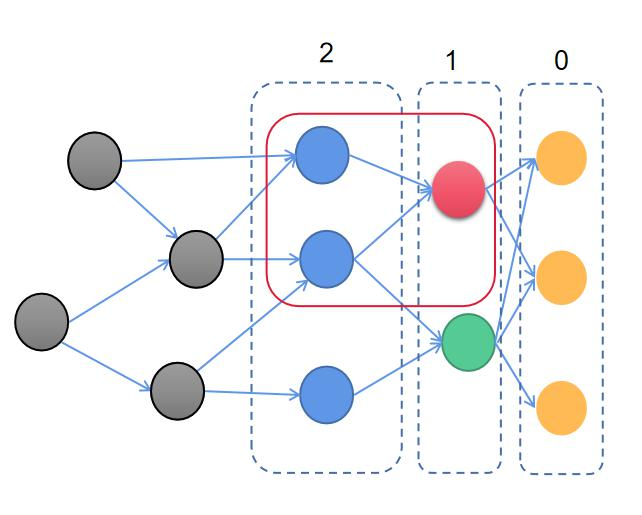
\includegraphics[width=0.6\textwidth]{Img/ft2.png}
    \caption{出错场景快速恢复}
    \label{fig:ft2}
\end{figure}


\begin{figure}[htbp]
    \centering
    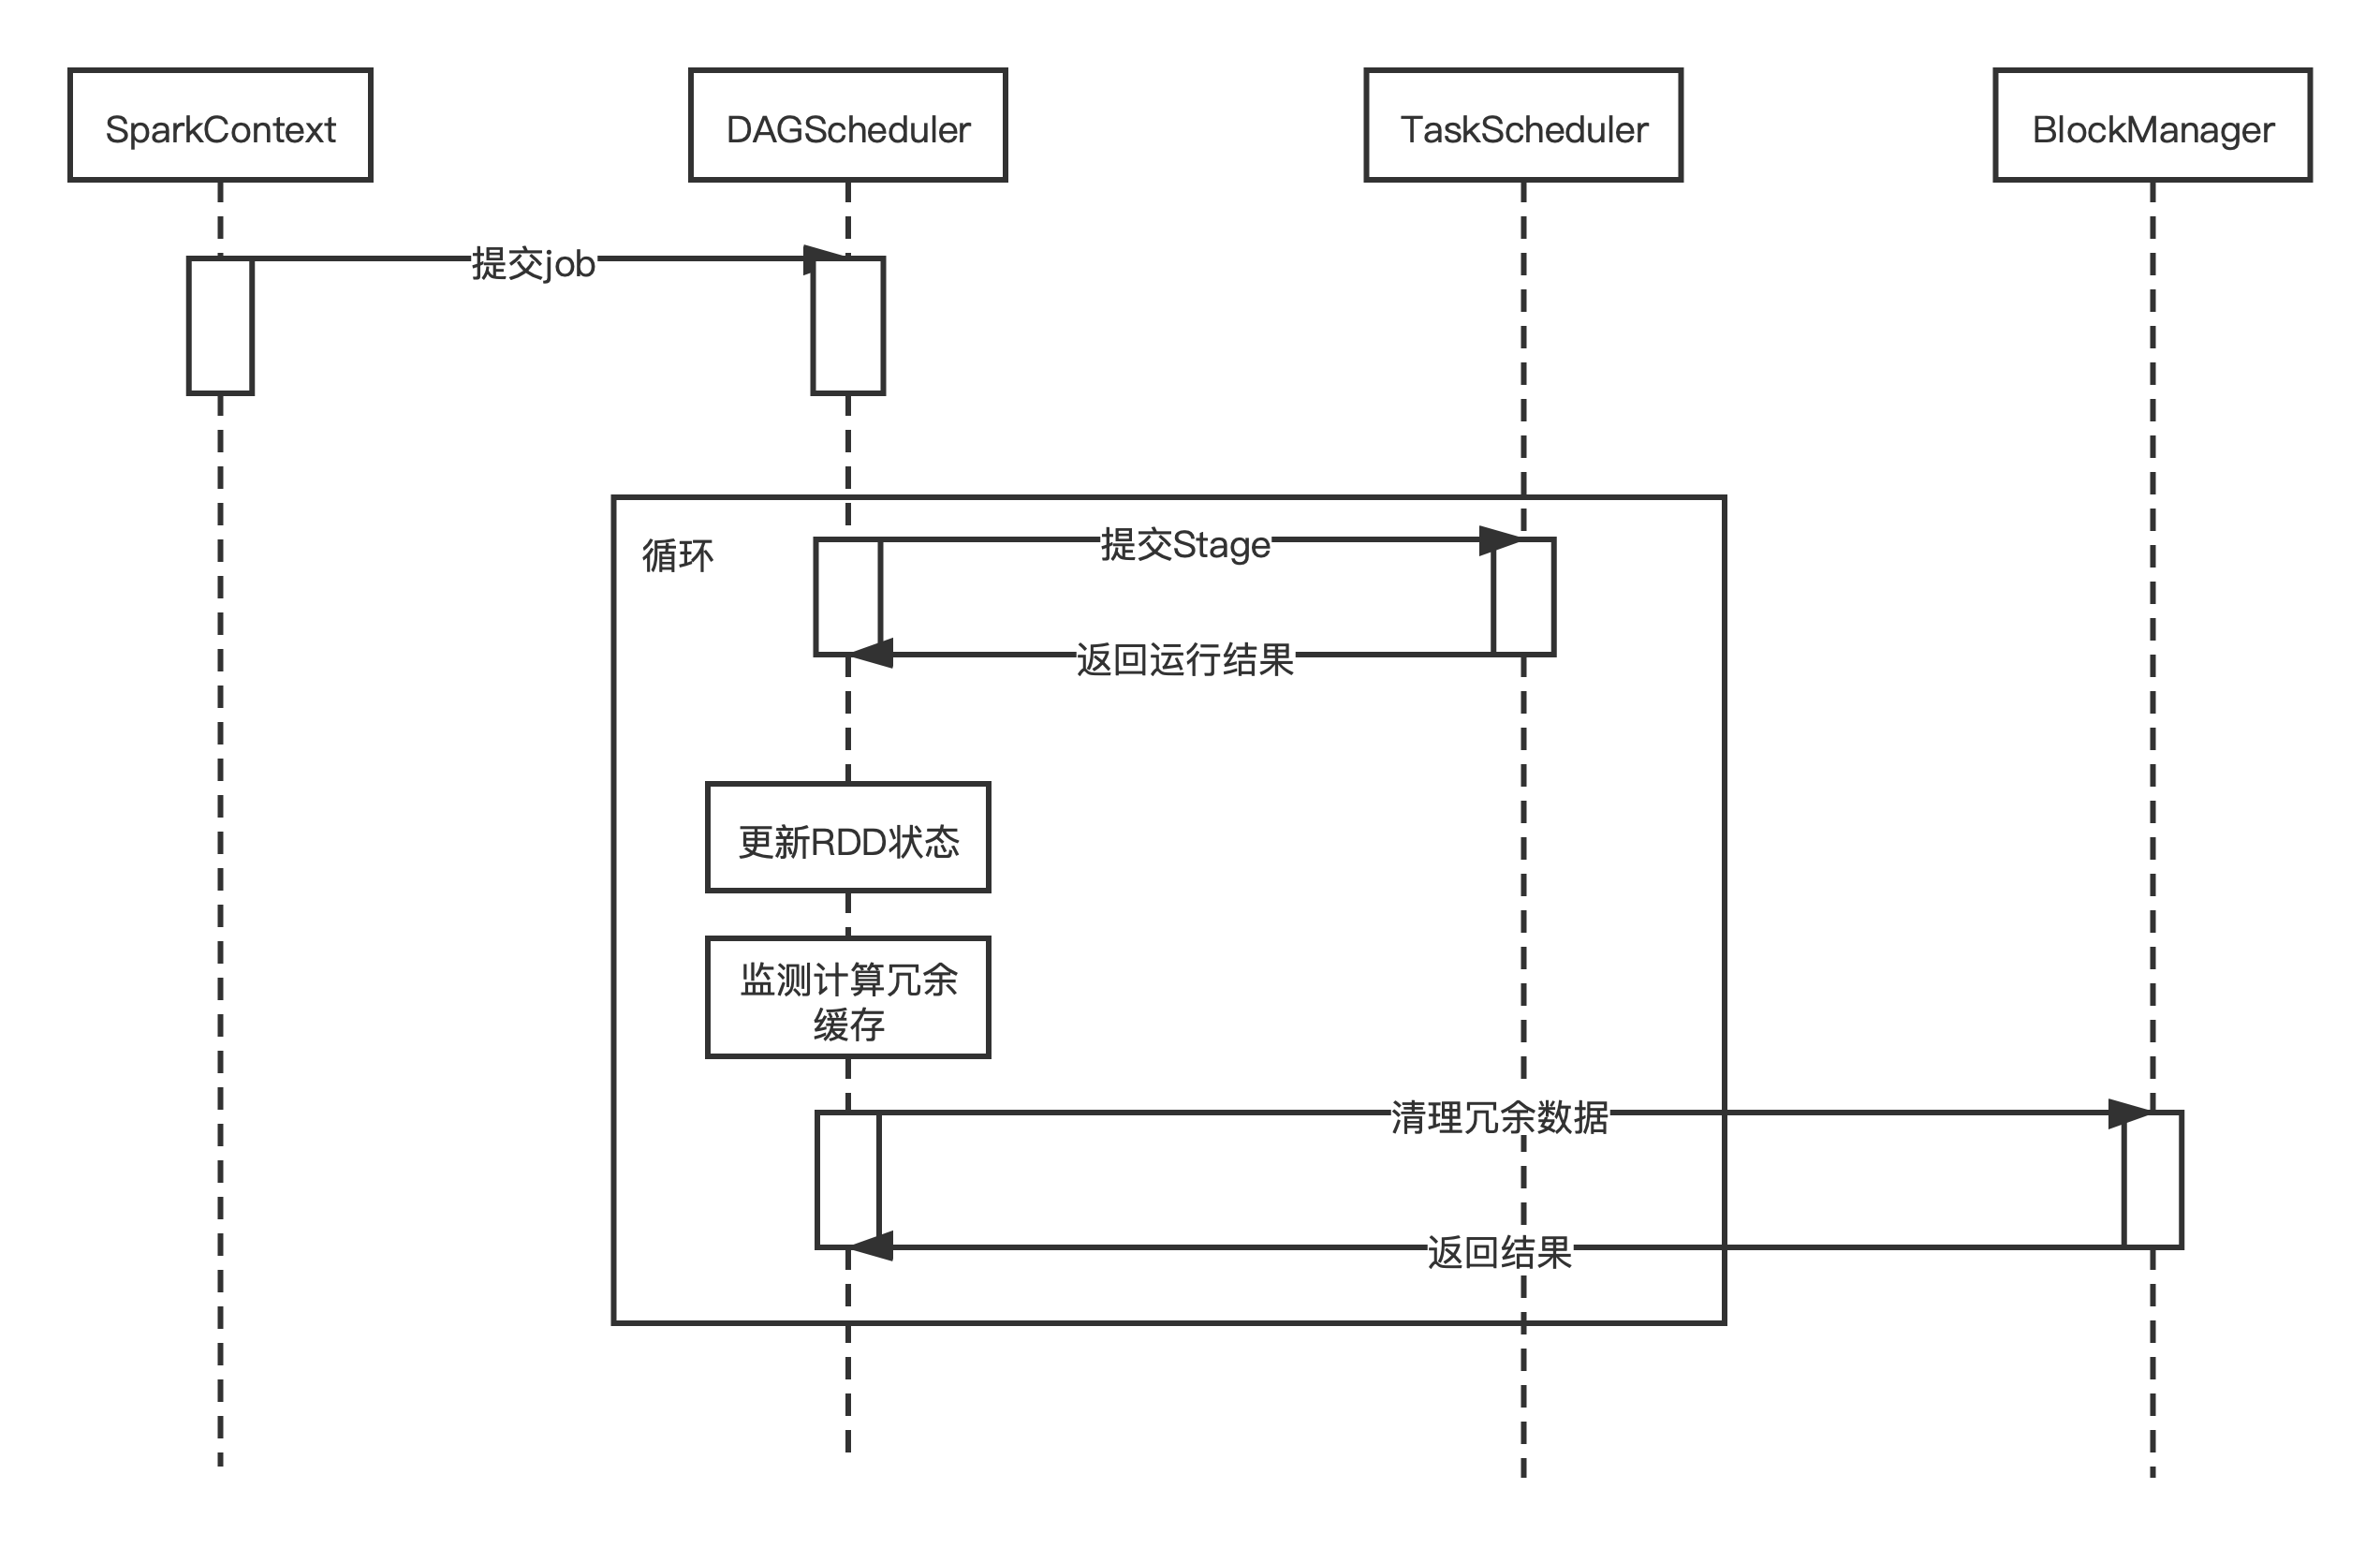
\includegraphics[width=1\textwidth]{Img/缓存清理模块流程图.png}
    \caption{缓存清理模块流程图}
    \label{fig:clean}
\end{figure}

\begin{algorithm}  
    \caption{缓存清理算法}  
    \begin{algorithmic}[1] %每行显示行号  
        \Require 正在计算的RDD节点列表
        \Ensure 需要清理的数据节点
        \Function{CLEAN\_CACHE}{$ARRAY<RDD> \ rdds$}
            \State $queue \gets \ new \ Queue()$
            \State $dis \gets  \ new \ HashMap()$
            \State $cleanRdds \gets \ new \ Array()$
            \For{$rdd \in rdds$}
                \State $queue.enqueue(rdd)$
                \State $dis[rdd] \gets 0$
            \EndFor
            \While{$!queue.isEmpty()$}
                \State $rdd \gets queue.pop()$
                \State $predecessors \gets rdd.getPredecessors()$
                \For{$predecessor \in predecessors$}
                    \State $queue.enqueue(predecessor)$
                    \State $dis[predecessor] \gets dis[rdd]+1$
                    \If{$dis[predecessor] > 2 \ AND \ predecessor.SRORAGE\_LEVEL == MEMORY\_ONLY$}
                        $cleanRdds.append(predecessor)$
                    \EndIf
                \EndFor
            \EndWhile
        \EndFunction
    \end{algorithmic}
    \label{alg:cal-dis}
\end{algorithm}

\section{测试与分析}

本章选取了逻辑回归、HIVE SQL、PageRank和矩阵分解8GB输入数据进行测试。选取8GB数据是因为测试环境Executor设置为8GB。2G和4G测试数据太少,用不完缓存空间。但是对于16GB测试数据会从一开始就用满Executor所有内存。所以使用8GB测试数据比较合适。根据图\ref{memory-use}测试结果可以发现,HIVE SQL冗余缓存清理效果最佳,这是应为HIVE SQL计算图是DAG形式,前面的数据计算结束之后就可以替换删除。而对于另外三种迭代式计算,因为迭代轮数很多,每次迭代都会将数据缓存到内存之中,又因为内存释放又延迟,所以虽然缓存清理有一定效果,但是逐渐的内存也会被占满。

\begin{figure}[!htbp]
    \centering
    \begin{subfigure}[b]{0.45\linewidth}
      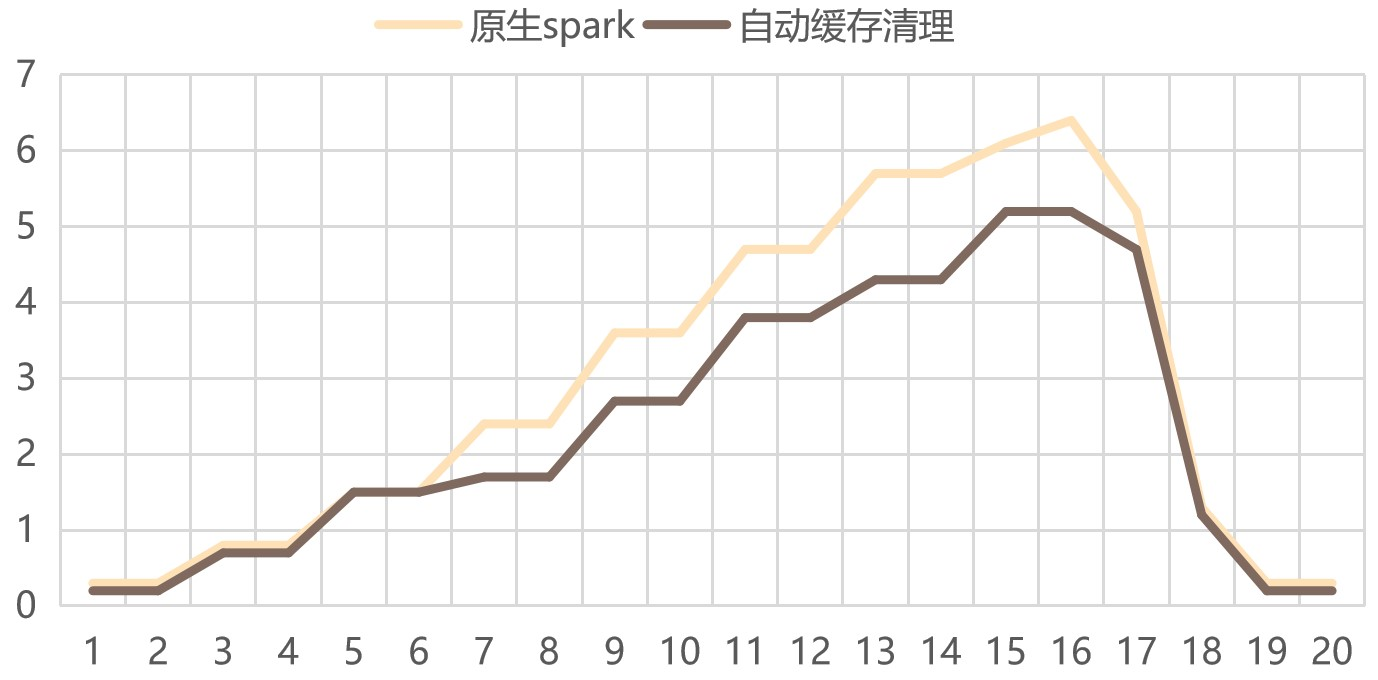
\includegraphics[width=\textwidth]{Img/lr-use.jpg}
      \caption{逻辑回归内存使用情况}
      \label{fig:lr-use}
    \end{subfigure}%
    ~% add desired spacing
    \begin{subfigure}[b]{0.45\linewidth}
      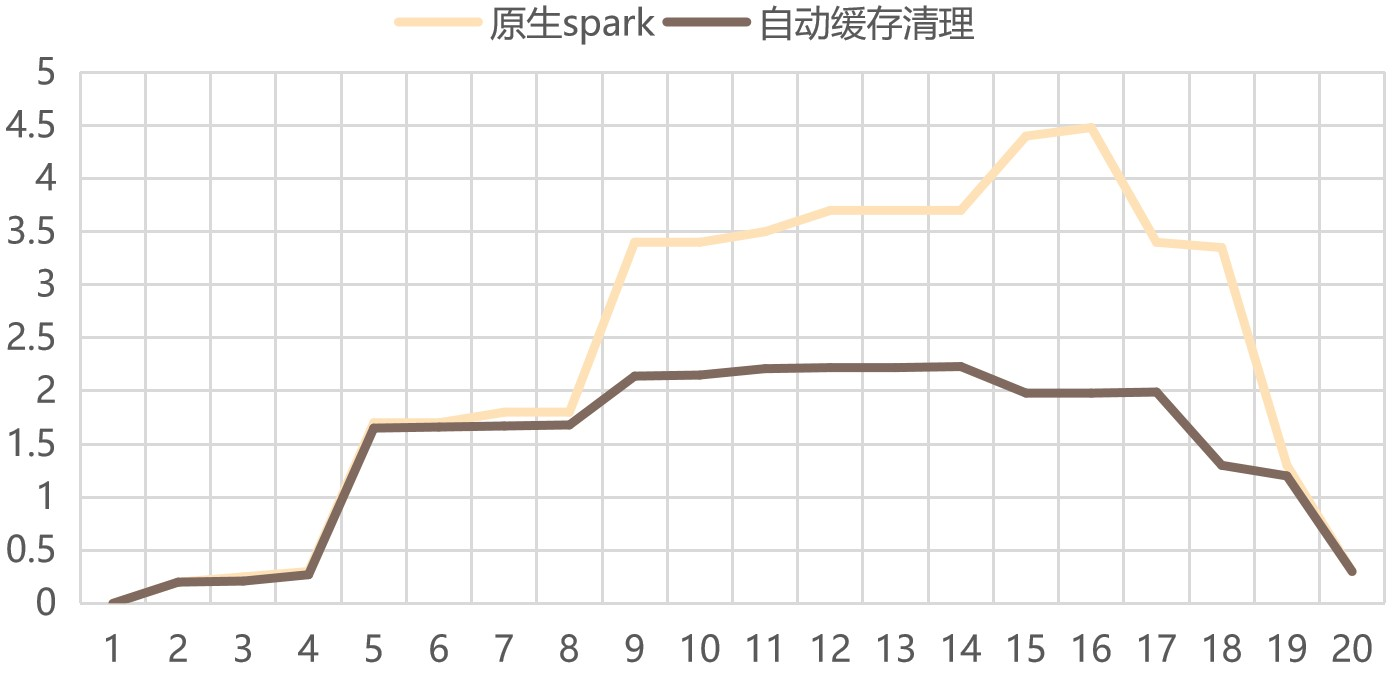
\includegraphics[width=\textwidth]{Img/hive-use.jpg}
      \caption{HIVE SQL内存使用情况}
      \label{fig:hive-use}
    \end{subfigure}
    \\% line break
    \begin{subfigure}[b]{0.45\linewidth}
      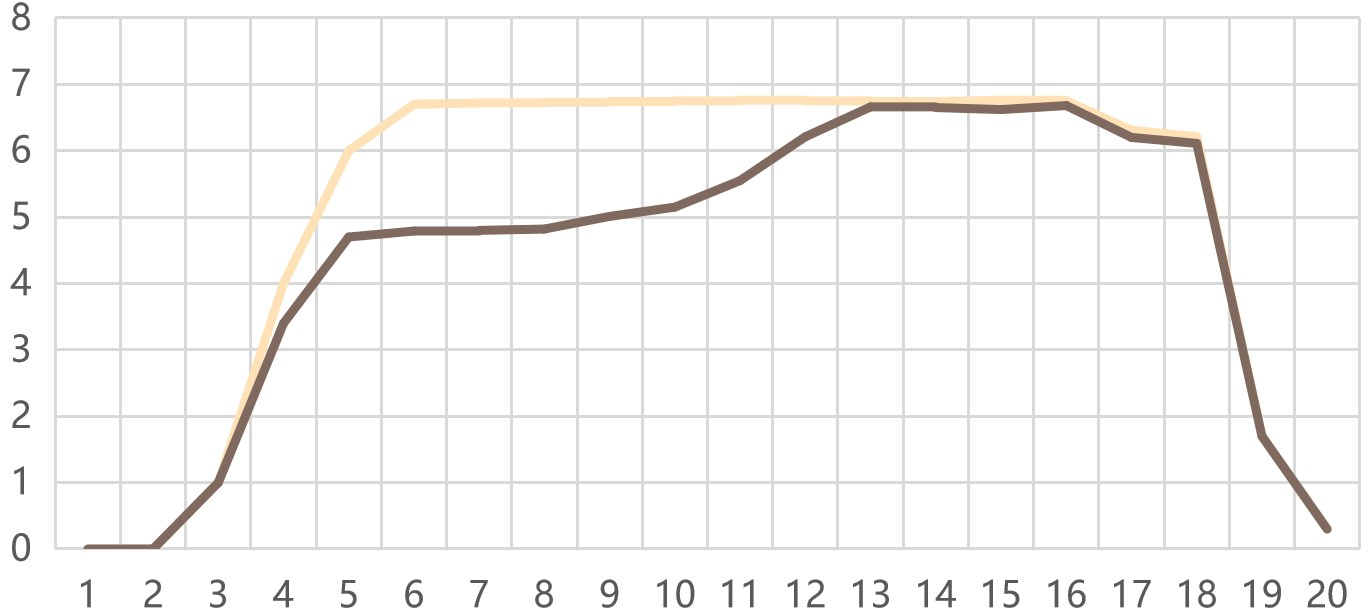
\includegraphics[width=\textwidth]{Img/pagerank-use.jpg}
      \caption{PageRank内存使用情况}
      \label{fig:pagerank-use}
    \end{subfigure}%
    ~% add desired spacing
    \begin{subfigure}[b]{0.45\linewidth}
      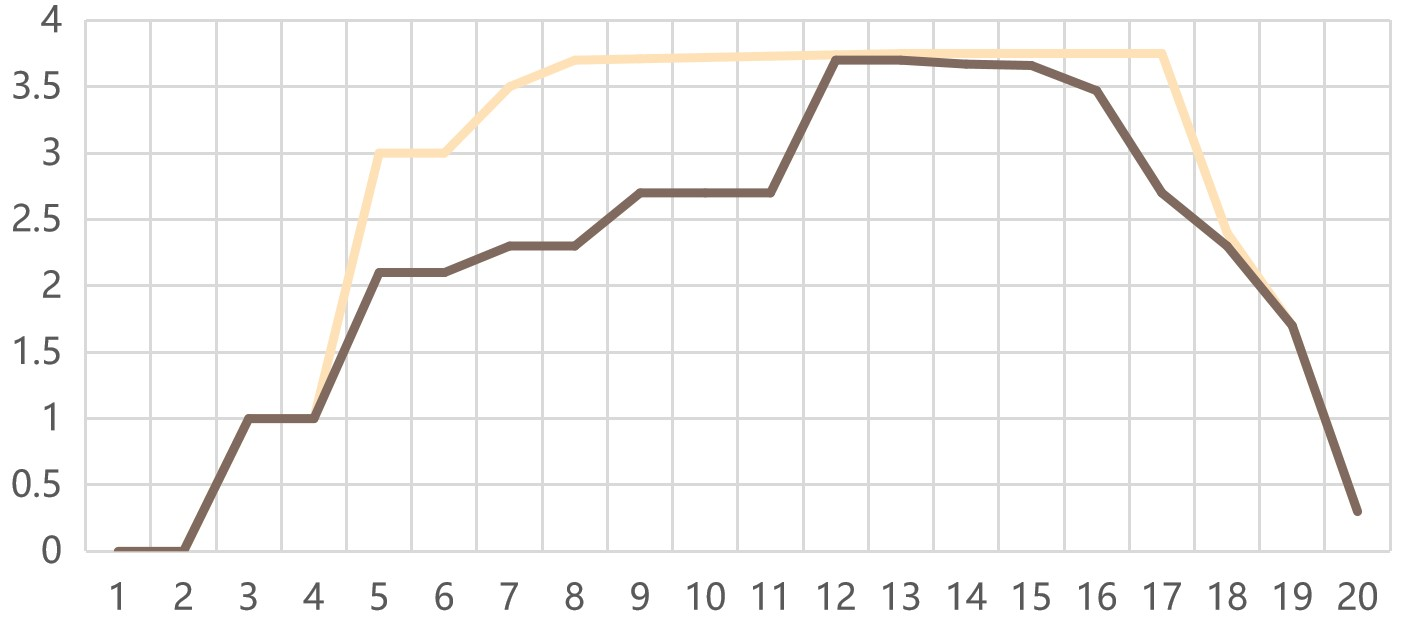
\includegraphics[width=\textwidth]{Img/matrix-use.jpg}
      \caption{矩阵分解内存使用情况}
      \label{fig:matrix-use}
    \end{subfigure}
    \caption{内存使用情况测试}
    \label{fig:memory-use}
\end{figure}

\section{本章总结}

本章首先介绍了Spark内存管理模块底层原理以及JVM垃圾回收的简单原理,然后分析了潜在的问题。为了解决潜在的OOM问题并且保证一定的兼容性,本文提出了一种容错性加强的缓存清理方法。最后进行了一些列测试。测试发现对于迭代计算作业,在作业开始时缓存清理模块能够减少内存使用量,但是逐渐的还是会占满所有缓存空间。缓存清理模块对于SQL查询作业效果比较好,因为SQL作业为DAG图结构,阶段性特性比较好,所以能够解决大量的内存空间。
\chapter{总结与展望}\label{chap:guide}

\section{本文总结}

\section{研究展望}

\input{Tex/Chap_Intro}
\input{Tex/Chap_Guide}
%---------------------------------------------------------------------------%
% main content
%-
%-> Appendix
%-
\cleardoublepage%
\appendix% initialize the environment
% \chapter{中国科学院大学学位论文撰写要求}

% 学位论文是研究生科研工作成果的集中体现,是评判学位申请者学术水平、授予其学位的主要依据,是科研领域重要的文献资料。根据《科学技术报告、学位论文和学术论文的编写格式》(GB/T 7713-1987)、《学位论文编写规则》(GB/T 7713.1-2006)和《文后参考文献著录规则》(GB7714—87)等国家有关标准,结合中国科学院大学(以下简称“国科大”)的实际情况,特制订本规定。

% \section{论文无附录者无需附录部分}

% \section{测试公式编号 \texorpdfstring{$\Lambda,\lambda,\theta,\bar{\Lambda},\sqrt{S_{NN}}$}{$\textLambda,\textlambda,\texttheta,\bar{\textLambda},\sqrt{S_{NN}}$}} \label{sec:testmath}

% \begin{equation} \label{eq:appedns}
%     \adddotsbeforeeqnnum%
%     \begin{cases}
%         \frac{\partial \rho}{\partial t} + \nabla\cdot(\rho\Vector{V}) = 0\\
%         \frac{\partial (\rho\Vector{V})}{\partial t} + \nabla\cdot(\rho\Vector{V}\Vector{V}) = \nabla\cdot\Tensor{\sigma}\\
%         \frac{\partial (\rho E)}{\partial t} + \nabla\cdot(\rho E\Vector{V}) = \nabla\cdot(k\nabla T) + \nabla\cdot(\Tensor{\sigma}\cdot\Vector{V})
%     \end{cases}
% \end{equation}
% \begin{equation}
%     \adddotsbeforeeqnnum%
%     \frac{\partial }{\partial t}\int\limits_{\Omega} u \, \mathrm{d}\Omega + \int\limits_{S} \unitVector{n}\cdot(u\Vector{V}) \, \mathrm{d}S = \dot{\phi}
% \end{equation}
% \[
%     \begin{split}
%         \mathcal{L} \{f\}(s) &= \int _{0^{-}}^{\infty} f(t) e^{-st} \, \mathrm{d}t, \ 
%         \mathscr{L} \{f\}(s) = \int _{0^{-}}^{\infty} f(t) e^{-st} \, \mathrm{d}t\\
%         \mathcal{F} {\bigl (} f(x+x_{0}) {\bigr )} &= \mathcal{F} {\bigl (} f(x) {\bigr )} e^{2\pi i\xi x_{0}}, \ 
%         \mathscr{F} {\bigl (} f(x+x_{0}) {\bigr )} = \mathscr{F} {\bigl (} f(x) {\bigr )} e^{2\pi i\xi x_{0}}
%     \end{split}
% \]

% mathtext: $A,F,L,2,3,5,\sigma$, mathnormal: $A,F,L,2,3,5,\sigma$, mathrm: $\mathrm{A,F,L,2,3,5,\sigma}$.

% mathbf: $\mathbf{A,F,L,2,3,5,\sigma}$, mathit: $\mathit{A,F,L,2,3,5,\sigma}$, mathsf: $\mathsf{A,F,L,2,3,5,\sigma}$.

% mathtt: $\mathtt{A,F,L,2,3,5,\sigma}$, mathfrak: $\mathfrak{A,F,L,2,3,5,\sigma}$, mathbb: $\mathbb{A,F,L,2,3,5,\sigma}$.

% mathcal: $\mathcal{A,F,L,2,3,5,\sigma}$, mathscr: $\mathscr{A,F,L,2,3,5,\sigma}$, boldsymbol: $\boldsymbol{A,F,L,2,3,5,\sigma}$.

% vector: $\Vector{\sigma, T, a, F, n}$, unitvector: $\unitVector{\sigma, T, a, F, n}$

% matrix: $\Matrix{\sigma, T, a, F, n}$, unitmatrix: $\unitMatrix{\sigma, T, a, F, n}$

% tensor: $\Tensor{\sigma, T, a, F, n}$, unittensor: $\unitTensor{\sigma, T, a, F, n}$ 

% \section{测试生僻字}

% 霜蟾盥薇曜灵霜颸妙鬘虚霩淩澌菀枯菡萏泬寥窅冥毰毸濩落霅霅便嬛岧峣瀺灂姽婳愔嫕飒纚棽俪緸冤莩甲摛藻卮言倥侗椒觞期颐夜阑彬蔚倥偬澄廓簪缨陟遐迤逦缥缃鹣鲽憯懔闺闼璀错媕婀噌吰澒洞阛闠覼缕玓瓑逡巡諓諓琭琭瀌瀌踽踽叆叇氤氲瓠犀流眄蹀躞赟嬛茕頔璎珞螓首蘅皋惏悷缱绻昶皴皱颟顸愀然菡萏卑陬纯懿犇麤掱暒 墌墍墎墏墐墒墒墓墔墕墖墘墖墚墛坠墝增墠墡墢墣墤墥墦墧墨墩墪樽墬墭堕墯墰墱墲坟墴墵垯墷墸墹墺墙墼墽垦墿壀壁壂壃壄壅壆坛壈壉壊垱壌壍埙壏壐壑壒压壔壕壖壗垒圹垆壛壜壝垄壠壡坜壣壤壥壦壧壨坝塆圭嫶嫷嫸嫹嫺娴嫼嫽嫾婳妫嬁嬂嬃嬄嬅嬆嬇娆嬉嬊娇嬍嬎嬏嬐嬑嬒嬓嬔嬕嬖嬗嬘嫱嬚嬛嬜嬞嬟嬠嫒嬢嬣嬥嬦嬧嬨嬩嫔嬫嬬奶嬬嬮嬯婴嬱嬲嬳嬴嬵嬶嬷婶嬹嬺嬻嬼嬽嬾嬿孀孁孂娘孄孅孆孇孆孈孉孊娈孋孊孍孎孏嫫婿媚嵭嵮嵯嵰嵱嵲嵳嵴嵵嵶嵷嵸嵹嵺嵻嵼嵽嵾嵿嶀嵝嶂嶃崭嶅嶆岖嶈嶉嶊嶋嶌嶍嶎嶏嶐嶑嶒嶓嵚嶕嶖嶘嶙嶚嶛嶜嶝嶞嶟峤嶡峣嶣嶤嶥嶦峄峃嶩嶪嶫嶬嶭崄嶯嶰嶱嶲嶳岙嶵嶶嶷嵘嶹岭嶻屿岳帋巀巁巂巃巄巅巆巇巈巉巊岿巌巍巎巏巐巑峦巓巅巕岩巗巘巙巚帠帡帢帣帤帨帩帪帬帯帰帱帲帴帵帷帹帺帻帼帽帾帿幁幂帏幄幅幆幇幈幉幊幋幌幍幎幏幐幑幒幓幖幙幚幛幜幝幞帜幠幡幢幤幥幦幧幨幩幪幭幮幯幰幱庍庎庑庖庘庛庝庠庡庢庣庤庥庨庩庪庬庮庯庰庱庲庳庴庵庹庺庻庼庽庿廀厕廃厩廅廆廇廋廌廍庼廏廐廑廒廔廕廖廗廘廙廛廜廞庑廤廥廦廧廨廭廮廯廰痈廲廵廸廹廻廼廽廿弁弅弆弇弉弖弙弚弜弝弞弡弢弣弤弨弩弪弫弬弭弮弰弲弪弴弶弸弻弼弽弿彖彗彘彚彛彜彝彞彟彴彵彶彷彸役彺彻彽彾佛徂徃徆徇徉后徍徎徏径徒従徔徕徖徙徚徛徜徝从徟徕御徢徣徤徥徦徧徨复循徫旁徭微徯徰徱徲徳徴徵徶德徸彻徺忁忂惔愔忇忈忉忔忕忖忚忛応忝忞忟忪挣挦挧挨挩挪挫挬挭挮挰掇授掉掊掋掍掎掐掑排掓掔掕挜掚挂掜掝掞掟掠采探掣掤掦措掫掬掭掮掯掰掱掲掳掴掵掶掸掹掺掻掼掽掾掿拣揁揂揃揅揄揆揇揈揉揊揋揌揍揎揑揓揔揕揖揗揘揙揤揥揦揧揨揫捂揰揱揲揳援揵揶揷揸揻揼揾揿搀搁搂搃搄搅搇搈搉搊搋搌搎搏搐搑搒摓摔摕摖摗摙摚摛掼摝摞摠摡斫斩斮斱斲斳斴斵斶斸旪旫旮旯晒晓晔晕晖晗晘晙晛晜晞晟晠晡晰晣晤晥晦晧晪晫晬晭晰晱晲晳晴晵晷晸晹晻晼晽晾晿暀暁暂暃暄暅暆暇晕晖暊暋暌暍暎暏暐暑暒暓暔暕暖暗旸暙暚暛暜暝暞暟暠暡暣暤暥暦暧暨暩暪暬暭暮暯暰昵暲暳暴暵
% appendix content
%-
%-> Backmatter: bibliography, glossary, index
%-
\backmatter% initialize the environment
\intotoc*{\cleardoublepage}{\bibname}% add link to toc
\bibliography{Biblio/ref}% bibliography
%---------------------------------------------------------------------------%
%->> Backmatter
%---------------------------------------------------------------------------%
\chapter{作者简历及攻读学位期间发表的学术论文与研究成果}

\section*{作者简历}

汤瑞,男,中国科学院大学2018级硕士研究生,就读于中国科学院计算技术研究所高性能中心。

\section*{申请或已获得的专利:}

\begin{enumerate}
    \item 谭光明,汤瑞,邵恩. ⼀种⼯作流作业优先级计算以及节点调度控制⽅法,中国,202010063983.8.
    \item 谭光明,汤瑞,邵恩. ⼀种具有业务快速恢复功能的容器组更新系统
\end{enumerate}

\chapter[致谢]{致\quad 谢}\chaptermark{致\quad 谢}% syntax: \chapter[目录]{标题}\chaptermark{页眉}
\thispagestyle{noheaderstyle}% 如果需要移除当前页的页眉
%\pagestyle{noheaderstyle}% 如果需要移除整章的页眉

时光荏苒,三年光阴如梭,在本文完成之际,三年研究生生涯也即将结束。在这即将毕业的时刻,我心中有着对未来工作的希冀,在这三年的时光中,在学习,工作,科研和生活方面,我都收获了巨大的成长。我心中深知我的成长不仅仅有我自己的努力,更多需要感谢导师的细心指点,母校悉心教诲,还有家人同学朋友共同地支持和帮助。所以我在此表达衷心地感谢。

首先,我要感谢我的导师—谭光明教授。谭老师学识渊博,严谨认真。在学术研究方面和工作生活方面谭老师都给予了我巨大的支持和帮助。从选择研究方向,到毕业设计开题、中期答辩。每次我遇到问题,谭老师都会在百忙之际抽出时间对我悉心教导,每次我都受益匪浅。在此对谭老师表达深深的感谢。

感谢邵恩老师,邵恩老师尽心尽力,认真辅导课题组每个学生的学习和研究。在实验室的时间邵老师总是认真负责地指点研究方向,讨论研究思路,在专利、论文、毕设开题、中期的准备过程中,邵老师总是认真地帮我修改内容。邵老师认真负责的工作态度深深地鼓舞了我。同时在生活方面邵老师也给与了很多帮助,在这里对邵老师表示衷心地感谢。

感谢实验室以及计算所所有老师,在计算所的三年时间里各位老师都对我提供了或多或少的帮助。感谢实验室所有师兄师姐师弟师妹,在这三年中我们一起努力,相互帮助,都收获了很大的成长。

感谢家人与朋友对我的关系和支持,每当我心情低落沉闷时,都是你们在身边鼓励我支持我。

最后,再次感谢各位老师和同学,感谢百忙之中参加答辩和论文评阅的老师!

\cleardoublepage[plain]% 让文档总是结束于偶数页,可根据需要设定页眉页脚样式,如 [noheaderstyle]
%---------------------------------------------------------------------------%
% other information
\end{document}
%---------------------------------------------------------------------------%

